\documentclass[12pt,pdftex]{article}
\usepackage[pdftex]{graphicx,color}
\usepackage{setspace,palatino,multirow}
\usepackage{amsmath,amssymb}
\usepackage{titlesec}
\usepackage{lscape}
%\usepackage{subfigure}
\usepackage{threeparttable}
\usepackage{natbib}
\bibliographystyle{ecta}
\usepackage{cite}
\usepackage{booktabs}
\usepackage{subcaption}
\usepackage{pdflscape}
\usepackage{afterpage}
\usepackage{xcolor}
\usepackage{rotating}

\definecolor{nblue}{RGB}{0,0,128}

\usepackage[pdftex,colorlinks=true, bookmarks=false,
pdfstartview={XYZ null null 0.65},
pdftitle={Heterogeneous Agent Trade},
pdfauthor={ Michael E. Waugh},
pdfkeywords={economics, trade, dynamics, quant econ, consumption, data science,
waugh, incomplete markets, inequality, julia, Armington, Minneapolis Fed, price elasticity, distance, python, matplotlib},
colorlinks=true,linkcolor=darkgray,citecolor=darkgray,urlcolor=darkgray,
breaklinks]{hyperref}

\newcounter{saveeqni}%
\newcounter{saveeqn01i}%
\newcommand{\alpheqni}{\setcounter{saveeqni}{\value{section}}%
%\setcounter{saveeqn01i}{\value{subsectioni}}%
\renewcommand{\theequation}
    {\alph{saveeqni}\mbox{.\arabic{equation}}}}%
\newcommand{\reseteqni}{\setcounter{equation}{\value{saveeqni}}%
\renewcommand{\theequation}{\arabic{equation}}}%

\newtheorem{as}{Assumption}
\newtheorem{reg}{Regularity Condition}
\newtheorem{conjecture}{Conjecture}
\newtheorem{corr}{Corollary}
\newtheorem{df}{Definition}
\newtheorem{lemma}{Lemma}
\newtheorem{prp}{Proposition}
\newtheorem{rmk}{Remark}
\newenvironment{prf}{{\bf Proof}}{\hfill { }}

\DeclareMathOperator*{\plim}{plim}
\DeclareMathOperator*{\umax}{max}

\special{papersize=8.5in,11in}
\onehalfspacing
\setlength{\parindent}{0.1em}
\setlength{\parskip}{.09in}
\textwidth15.75cm
\evensidemargin 1.5in
\oddsidemargin 1.5in
\topmargin 8.5cm
\textheight 10in
\hyphenation{over-lapping}

\titleformat{\section}{\color{black}\large\bf}{\color{black}{\thesection.}}{.25cm}{}
\titleformat{\subsection}{\color{black}\normalsize\bf}{\thesubsection.}{.5em}{}
\titleformat{\subsubsection}{\color{black}\normalsize\bf}{\thesubsubsection.}{.5em}{}

\titlespacing{\section}{0pt}{*1.5}{*.5}
\titlespacing{\subsection}{0pt}{*1.5}{*.5}
\titlespacing{\subsubsection}{0pt}{*1.5}{*.5}

\def\thesection{\arabic{section}}
\def\thesubsection{\arabic{section}.\arabic{subsection}}
\def\thesubsubsection{\arabic{section}.\arabic{subsection}.\Alph{subsubsection}}

\def\citeapos#1{\citeauthor{#1}'s (\citeyear{#1})}

\renewcommand{\arraystretch}{1.1}
\usepackage[margin=2cm]{geometry}

\begin{document}

\begin{onehalfspacing}

{\large \textbf{\href{https://www.waugheconomics.com/uploads/2/2/5/6/22563786/heterogeneous-agent-trade.pdf}{Heterogeneous Agent Trade}}}

\vspace{0.5cm}

\href{http://www.waugheconomics.com/}{Michael E. Waugh} \\ Federal Reserve Bank of Minneapolis and NBER

\vspace{0.5cm}

\textbf{In Progress.} This draft: August 2023

\vspace{1.5cm}


\normalsize

ABSTRACT ------------------------------------------------------------------------------------------------------------

This paper studies the implications of household heterogeneity for trade. My model features household-level price ( trade ) elasticities that increase with a households' marginal utility of consumption. The gains from trade reflect a household's exposure to trade and its price elasticity. Thus, conditional on exposure, price reductions are more valuable for poor, high marginal utility households. Quantitatively, I calibrate the model to match bilateral trade flows for 19 countries and micro facts about household-level expenditure patterns and price elasticities. The gains from trade are pro-poor with the poorest households gaining six times more than the richest. The average gains from trade are nearly three times larger than representative agent benchmarks.

------------------------------------------------------------------------------------------------------------------------------
%%\vspace{0.25cm}
%
%%JEL Classification:
%%
%%
%%Keywords:

\vspace{6.0cm}

\footnotesize Email: michael.e.waugh@gmail.com. The views expressed herein are those of the author and not necessarily those of the Federal Reserve Bank of Minneapolis or the Federal Reserve System. This project was developed with research support from the National Science Foundation (NSF Award number 1948800). Thomas Hasenzagl provided excellent research assistance. My github repository provides the code and supplementary work behind this paper at \url{https://github.com/mwaugh0328/heterogeneous-agent-trade}.

\hspace{-0.05cm}



\thispagestyle{empty}
\newpage
\normalsize

This paper studies the implications of household heterogeneity for trade. From the perspective of trade, household heterogeneity is interesting because of the notion that some benefit from trade and others don't. One aspect of these unequal gains relates to the idea that rich and poor consumers have different sensitivities to price and, thus, they shape the gains from trade.  I develop this idea in a model that results in heterogenous price sensitivity and I study it's implications for trade qualitatively and quantitatively.

The core issue in my model is that heterogeneity in price sensitivity reflects heterogeneity in the marginal utility of consumption across households. Then even if rich and poor households are equally exposed to changes in prices | heterogeneity in price sensitivity implies that they value a price change differently. Thus, poor, high marginal utility households | who are very sensitive to price | benefit more from trade than rich households. Quantitatively, I find that this mechanism is powerful with the poorest households gaining six times more than the richest. And the average gains from trade are nearly three times larger than standard, representative agent benchmarks.

The model that I develop builds upon workhorse frameworks. Trade in goods follows the Armington tradition with producers in each country producing a national variety. The important twist is that households have random utility over these varieties and they make a discrete choice over the varieties to consume (\citet{mcfadden1974frontiers}).  Household heterogeneity is induced via the standard incomplete markets model (\citet{bewley1979optimum}, \citet{imrohorouglu1989cost}, \citet{huggett1993risk}, \citet{aiyagari1994uninsured}) with households facing incomplete insurance against idiosyncratic productivity and taste shocks. This setting naturally leads to dispersion the marginal utility of consumption.

Together, the discrete choice and incomplete markets model interact with the key force being household-level trade (price) elasticities that vary with income and wealth. Income and wealth matter because a household's price sensitivity, in essence, is about the marginal utility of consumption. Poor, high marginal utility households strongly value extra consumption independent of the variety and, thus, they are very sensitive to price. In contrast, rich households' marginal utility is low, are less sensitive to changes in prices, and likely consume their ideal variety independent of price. The distribution of households | how many rich and poor people are in a country | then determines the aggregate response of economy to changes in trade frictions and the aggregate pattern of trade.

The issues behind heterogeneity in price sensitivity leads to new perspectives on the welfare gains from trade. First, I show how one aspect of the gains from trade reflect the expected, discounted stream of changes in a household's home choice probability, similar in spirit to the result of \citet*{arkolakis2012new}. Unpacking this component reveals that the change in the home choice probability is essentially about two forces: (i) how exposed a household is to trade through its expenditure shares and (ii) its own price elasticity. Because the elasticity part reflects the marginal utility of consumption, the elasticity effect delivers the intuitive idea that one aspect of the gains from trade is a households' individual valuation of the price reduction. So even if a rich and poor household have similar expenditure patterns, the reduction in price is more valuable on the margin for the poor, high marginal utility households.

In addition to these insights, an additional new force behind the gains from trade emerges from my model, i.e., how a liberalization changes a household's valuation of its net asset position. The issue is that a trade liberalization will change interest rates and lead to winners and losers depending upon a households' net asset position. For example, if a trade liberalization leads to an increase in interest rates, net debtors suffer since their terms to borrow deteriorated, while net savers benefit. And this force is connected with the ideas above because any change in these valuation affects are multiplied by the marginal utility of consumption.

Before moving on to the quantitative work, I explore two special cases to highlight the role that market incompleteness and preferences play in shaping these results. The first case is the efficient allocation where a planner can reallocate resources and overcome market incompleteness. In this case, I recover ``first-best intuition'' with the gains from trade only reflecting the direct savings associated with a reduction in trade costs. In this allocation, changes in expenditure patterns are not relevant via an envelope theorem argument | the planner already sources goods from the correct places so there are no gains from expenditure switching. And heterogeneity in a household's valuations of gains are irrelevant because marginal utility is equated. While my economy is about heterogeneity on the household side, this result is reminiscent of \citet{AtkesonBurstein2010} and the irrelevance of firm heterogeneity in an economy where the allocation is efficient. Thus, the core issues at play in my model are not household heterogeneity per se, but inefficiencies induced by market incompleteness.

The second special case is when the utility function over the physical commodity is $\log$. With $\log$ utility, I obtain a separation result where aggregate trade outcomes ``separate'' from household heterogeneity. Trade takes a constant elasticity form with the trade elasticity pinned down by the dispersion parameter on the taste shocks similar to \citet{eaton2002technology}. And the trade elasticity and the share of home purchases summarize the gains from trade like in \citet{arkolakis2012new}. This case is also interesting because \citet*{anderson1987ces} showed that in a static model with log utility and additive logit shocks, the economy behaves \emph{as if} there were a representative agent CES consumer. In my economy, my suspicion was that market incompleteness and intertemporal behavior would nullify \citeapos{anderson1987ces} result|it does not.

Quantitatively, I make a contribution by computing and calibrating the model at a scale typically reserved for static trade models. As a testing ground, I focus on the data set of \citet{eaton2002technology}. The 19 countries in this data set is about the right size to easily illustrate how a very rich model like this can work in a multi-country setting. Moreover, the \citet{eaton2002technology} data set provides a well defined benchmark disciplined by bilateral trade flows and gravity variables|so it's a nice laboratory to explore new issues in.

The calibration challenge is the following. The model does not admit a gravity representation that allows researchers to invert trade frictions and productivity levels from trade flows as done in \citet{eaton2002technology} and many subsequent papers. Similarly, the model does not admit the use of exact-hat algebra which allows the research to construct counterfactuals without the knowledge of primitives like trade frictions or productivity (see, e.g., \citet{costinot2014trade} or the dynamic extension in \citet*{caliendo2015trade}).

My solution is to use the insight that the regressions employed in gravity frameworks provide very accurate descriptions of the data generating process. Rather than treating the gravity regression as a structural relationship, I use it as a ``guide'' and use an indirect inference procedure where I estimate parameters of the model so that the regression coefficients from a standard gravity regression run on my model's data match that seen in the data. This procedure works well and, thus, the model is able to match spatial distribution of economic activity in the data|just as well as standard, constant elasticity gravity models.

An outcome of the calibration is that aggregate trade elasticities decrease with the competitiveness of a source country in a destination. In other words, expensive products are more elastic relative to cheaper products | in aggregate. Behind this is what some might call a super-elasticity of trade within the model \emph{endogenously} delivering the result that elasticities increases with price and a pattern conforming with ``Marshall's Second Law of Demand'' or in the language of \citet{mrazova2017not} aggregate demand functions turn out to be ``subconvex'' relative to CES demand.



Motivating my work has been a sequence of papers focusing on measuring the heterogenous impacts of trade on the consumer side. \citet{fajgelbaum2016measuring}, \citet{carroll2020heterogeneous}, \citet{borusyak2021distributional}, \citet{jaccardtoronto} are recent examples that measure heterogeneity in import exposure.\footnote{Its important for the reader to distinguish the pattern of heterogeneity across sectors vs. within a sector (\citet{cravino2017distributional} makes this distinction very clear). The evidence suggests that the patterns work in different directions with poor households consuming more traded goods, but within traded goods the poor consume lower price varieties and less imported content. My model is of one sector and about expenditure and substitution within that one sector.} \citet*{auer2022unequal} and \citet*{colicev2022impact} go a step further measuring heterogeneity in price sensitivity across the income distribution and this type of evidence is very much the launching point for my paper.

While this work motivates my paper, I take a conceptually different approach. Rather than focusing on measurement, I develop a model of household heterogeneity that endogenously delivers heterogeneity in price elasticities and study its implications. In this sense, my papers approach is most similar to \citet*{fajgelbaum2011income} who study how inequality and non-homotheticities shape trade in vertically differentiated products. A unique aspect of my work is that I start with a theory behind the distribution of income and wealth. This theory plus a demand system with heterogenous price elasticities then breaks aggregation in the goods market. And because aggregation is broken, it opens the door to new insights about trade, the interaction of trade and financial markets, and how market incompleteness shapes the aggregate pattern of trade.

My paper also relates to a recent series of papers that combines trade models with heterogenous agent, incomplete market models. Some of this is my own work in \citet{lyon2018redistributing}, \citet{lyon2019}, \citet{waugh_consumption}; \citet*{gaston2018} and \citet{carroll2020heterogeneous} are important contributions as well. This class of papers primarily focuses on how heterogenous exposure through the labor market passes through to consumption and, thus, welfare. In this paper, I'm doing something different and it is an attempt to answer the question: does heterogeneity and market incompleteness matter for trade?

This paper also relates to a body of work focusing on the pricing implications in the presence of heterogenous price sensitivity. \citet{nakamura2010accounting} is an early example of a macro-style model with an IO-style demand system similar in spirit to my paper and they focuses on the implications for the incomplete pass through of shocks to prices. My own work in \citet{p-iq} is very much a companion piece to this paper with imperfect competition in product markets and it focuses on the heterogenous pass-through of supply and demand shocks into prices for different types of consumers. \citet{nord2022shopping} takes a search-theoretic approach, but the core issue is the same | how demand composition affects pricing decisions. With that said, this model simplifies matters by focusing on a world with perfect competition and, hence, I turn my focus on how household heterogeneity matters for trade.




% Connect with close economy stuff...evidence on prices


%because  within their respective literatures.
%
%
%
%
%%\footnote{Separate from this is computational challenge. Finding an equilibrium requires (i) solving for households dynamic problems|in each country (ii) constructing the stationary distribution of expenditure patterns and wealth|in each country (iii) aggregating and then (iv) finding a vector of prices so goods markets and financial markets clear world wide. Plot twist: It's doable. My github repository and the Appendix provides a complete description of my approach and methods.}
%
%
%then allows me to think explicitly about normative issues
%
%
%As a I show, market incompleteness is not a sufficient condition to




%Lit review:
%\begin{itemize}
%  \item FK paper, about heterogeneity in shares. This is about elasticities. They say model is pro-poor, but the issue is about sector. This is a model of within catagory/sector. Relates to Cravino Levchncho.
%
% \item Cravino Levchenko is about have a within discussion, they just don't see shares. But what they do see (in the is that high income guys buy high priced stuff). Then when constructing the price index, they assume this in some way. Simmilar to Krill. Key is to distingusih, income on price within varity, vs. income and shares (imported or not) and where they come from.

%  \item Note my formulas have similar flavor to fixed share approach. Planner is share times change is welfare gain. Need to look at krill paper.
%
%\item Krill paper... they do find that within category, rich buy more imported stuff than poor. The issue is complicated as you go across categories and then you do not get much action. The KN data set goes a deep dive and finds this as well. China is strange, strong case for thinking about qualit see Page 18 second to last paragraph. There you see the Armington quirk, imported stuff is more expensive, and rich guys are buying imported stuff. Other thing about Krill paper is critique of FK paper...AIDS generates a mechanical pro-poor bias. Non-homothetic CES is flexible to generate pattern in the data, FK is not. Final point, the Krill paper derives the share approach, this turns out to be exactly the same as the gains from trade in planner allocation
%
%\item Torston Jaccard does something simmilar to Krill, Auer. China messe stuff up, Europe strong pro rich exposure. All personal beuty products. Simmilar stuff to Auer. Proably more relavent for work with Simon is the stuff abour urban vs. rural and how this is above and beyond income, suggests something up about retailer. Does nested logit.
%
%\item The hotman paper is strange. This is mostly across sectors and claim they find something like Krill. No elasticity effect. Second, the Layspayers gives a totally different estimate than the model (inflation is high for poor vs rich) Why? Not really told that. The inflation results are suggestive that rich benefited more...but not quite obvious. Also not sure what the role of the firm is.
%
%\item Walsh paper...looks similar to my welfare calculations. Builds on the Moll paper too. Interesting is how they compute money metric by computing change in welfare relative to change in muc. Should put in labor income channel.
%
%\item Moll paper is very slick. Again more related than Walsh. One thing they do is put things in a money metric units by dividing through by muc in period 0. In the efficient economy, this then is back to Krill's formula. This money metric formula is why things are discounted by $R$ in Walsh...because the euler equation implies the ratio of muc's are equal to $R$. The other trick about this is that when assets are in zero net supply, the aggregate welfare gain in money metric units is zero. Key is that it's in money metric units though, in utils space there is true redistribution (worth talking about in either finacial globalization space or finacial autarky world).
%
%\item Is kind of related to Auclart...this the interest rate exposure channel. Less than I thought. As the key thing is more about dc. Tobin quote is nice about heterogenaity in muc. Everything is short term assets, so like in the moll paper sales = stocks. And then some people have different unhedge exposures to changes in interest rates.
%\end{itemize}


%This pattern of elasticities is consistent with recent evidence focusing on expenditure switching at the household level. \citet*{auer2022unequal} explore the heterogenous impact of the 2015 Swiss Franc appreciation and find that the exchange rate shock lead to larger changes in expenditure shares for poor households relative to the rich. In other words, poor households are more sensitive to price than rich households. Outside of the trade literature, there is broader set of evidence in support of the idea that price sensitivity declines with income; e.g. \citet{sangani2022markups} provides evidence in support of this fact using Nielsen Homescan data.
%%Discuss this evidence better. Faber Falley, Dellevingo,


\section{The Heterogeneous Agent Trade Model}

This section describes the model and then defines the decentralized competitive equilibrium. Trade is in the Armigton tradition with each country producing a nationally differentiated variety. Households face the ``income fluctuations problem'' as in the standard incomplete markets tradition (see, e.g., Chapter 17 of \citet{ljungqvist2012recursive}).

The key twist is that I do not employ modeling techniques with aggregation at household level across national varieties. Instead, I lean into the household heterogeneity and have households make a discrete choice over the varieties they consume in addition to their savings decisions. Aggregate trade flows, trade elasticities, and the gains from trade are then defined by the explicit aggregation of household-level decisions to purchase different varieties, their elasticity of demand, and their gains from trade.

\subsection{Production and Trade}\label{sec:trade}

There are $M$ locations which I call a country. Each country produces a nationally differentiated product. In country $i$, competitive firms' production technology to produce variety $i$ is:
\begin{align}
Q_i = A_i N_i,
\label{eq:production}
\end{align}
where $A_i$ is total factor productivity and $N_i$ are the efficiency units of labor supplied by households in country $i$.\footnote{Note that lack of physical capital in the model. Households here are saving in via pure exchange of non-state contingent IOUs as in \citet{huggett1993risk} rather than in physical capital as in \citet{aiyagari1994uninsured}.}

I focus on only one type of barrier to trade: there are iceberg trade costs $d_{ij} > 1$ for a good to go from supplier $j$ to buyer $i$.

Profit maximization of the producers in location $i$ results in the wage per efficiency unit reflecting the value of the marginal product of labor
\begin{align}
w_{i} = p_{i} A_{i}.
\label{eq:marginal-product}
\end{align}
Given iceberg trade costs, the unit cost for country $i$ to purchase a good from location $j$ is
\begin{align}
p_{ij} = \frac{d_{ij}w_{j}}{A_{j}}.
\label{eq:marginal-product-ship}
\end{align}
This is the trade and production side of the model. While sparse, it's worth reminding you that with a representative agent and a constant elasticity Armigton aggregator much comes out of this model. There is a gravity equation relating bilateral trade flows to country characteristics with a constant trade elasticity. And there are two sufficient statistics (the trade elasticity and home trade share) that globally characterize the welfare gains from trade. In the next section, I give up on the representative agent.

\subsection{Households}

There is a mass of $L_i$ households in each country. Households are immobile across countries. They are infinite lived and have time-sparable preferences over consumption of varieties:
\begin{align}
E_{0} \sum_{t = 0}^{\infty} \beta^{t} \tilde{u}( \{ c_{ijt} \}_{M}),
\end{align}
where the notation $\{ c_{ijt} \}_{M}$ means that the household has preferences over all $j$ varieties supplied by $M$ countries in the world. Here I'm indexing things by $ij$ to denote the variety $j$ that is consumed in location $i$ at date $t$.

Households' period utility function is of the random utility class and each period households can only consume one variety.\footnote{A more formal statement of preferences is that they $\tilde{u}( \{ c_{ijt} \}_{M}) = \sum_j \imath_{j} \tilde{u}( c_{ijt})$ where $\imath_{j}$ is an indicator function taking the value one if the consumer chooses variety $j$ and zero otherwise.} The utility associated with the choice of variety $j$ is
\begin{align}
\tilde{u}( c_{ijt} ) =  u(c_{ijt}) + \epsilon_{jt}. \label{eq:utility}
\end{align}
where the $\epsilon_{jt}$ are iid random variables across time, households, and countries. For the analysis, I assume that these shocks are distributed Type 1 Extreme Value with CDF
\begin{align}
F(\epsilon) &= \exp(-\exp(-\sigma_{\epsilon}^{-1}\epsilon))
\end{align}
where $\sigma_{\epsilon}$ is the dispersion parameter. A useful generalization of this setting to a multi-sector model is the ``infinite shopping isle'' approach of \citet{p-iq} where these shocks take on a Generalized Extreme Value representation and then households choose the sector and then the variety each period.

For now, all I assume is that the utility function over the physical good $c_{ijt}$ is well behaved. In the analysis below I explore different specifications of the utility function $u$ over the physical commodity. The canonical case for product markets (\citet{anderson1987ces}) or the spatial literature is where $u$ is $\log$ utility. Below, I highlight the rather curious properties of this case.

A household's efficiency units are stochastic and they evolve according to a Markov chain. So, $z$ is a household's efficiently units and $\mathcal{P}(z,z')$ describes the probability of a household with state $z$ efficiency units transiting to state $z'$. Again, I assume that $\mathcal{P}$ is well behaved in the necessary ways.

Households can save and borrow in a non-state contingent asset $a$ that is denominated in the units of the numeraire. One unit of the asset pays out with gross interest rate $R_i$ next period. I discuss this more in depth below, but the determination of $R_{i}$ is that which clears the bond market (local or global). A country specific, exogenous debt limit $\phi_{i}$ constrains borrowing so:
\begin{align}
a_{t+1} \geq - \phi_{i}.
\label{eq:borrowing-constraint}
\end{align}
All these pieces come together in the household's budget constraint, conditional on choosing variety $j$ to consume, and focusing on a stationary setting where prices are constant:
\begin{align}
p_{ij}c_{ijt} +  a_{t+1} \leq    R_{i} a_{t} + w_{i} z_{t}.\label{eq:trade-budget-constraint}
\end{align}
The value of asset purchases and consumption expenditures must be less than or equal to asset payments and labor earnings.

\subsection{The Household Problem}

The state variables of a individual household are its asset holdings and efficiency units. As alluded to above, for now I focus on a stationary setting where aggregates are not changing and, thus, I abstract from carrying the notation associated with them around.\footnote{If you \emph{do} want to carry them around, notice that all that households in each country care about are prices (today and in the future). The distributions of households in other countries, per se, don't matter. Thus, the relevant aggregate states in country $i$ are $\big [ \ \{ w_i \}_{M}, R_i \big ]$ which is the collection wage per efficiency units and the interest rate.}

The value function of a household in country $i$, after the variety shocks are realized, is
\begin{align}
v_{i}(a, z) = &  \max_{j} \big  \{ \  v_{i}(a, z, j)  \ \big \}
\label{eq:valuefun}
\end{align}
which is the maximum across the value functions associated with the discrete choices of different national varieties. The value function conditional on a choice of variety is
\begin{align}
v_{i}(a, z, j) = &  \max_{\ a' \ }\bigg  \{ u(c_{ij}) + \epsilon_{j}  + \beta \, \mathbb{E} [v_{i}(a', z')]  \bigg\}
\label{eq:value_fun_option} \\
\nonumber \\
\mbox{subject to}  \ & (\ref{eq:borrowing-constraint}) \  \mathrm{and} \ (\ref{eq:trade-budget-constraint}) \nonumber
\end{align}
where households choose asset holdings and the level of consumption is residually determined through the budget constraint. Associated with the solution to this problem is a policy function $g_{i}(a,z, j)$ which solves (\ref{eq:value_fun_option}) and maps current states into asset holdings tomorrow $a'$ contingent upon the variety choice $j$. Correspondingly, there is a consumption function $c_{i}(a,z, j)$ mapping states into consumption today, contingent upon the variety choice $j$.

The continuation value function on the right-hand side of (\ref{eq:value_fun_option}) is the expectation over (\ref{eq:valuefun}) with respect to (i) efficiency units next period, $z'$ and (ii) the variety taste shocks. An implication of this is that households understand that their may be situations where they really desire, say, a high priced imported good and, hence, save accordingly.

The Type 1 extreme value distribution on the taste shocks give rise to the following choice probabilities for each differentiated good:
\begin{align}
\pi_{ij}(a, z) = \exp \left( \frac{ v_{i}(a, z, j) }{\sigma_{\epsilon}} \right) \Bigg / \Phi_{i}(a,z), \label{eq:choice-prob} \\
\nonumber \\
\mbox{where} \ \ \ \Phi_{i}(a,z) := \sum_{j'} \exp \left( \frac{ v_{i}(a, z, j') }{\sigma_{\epsilon}} \right). \label{eq:big-phi}
\end{align}
which is the probability that a household with assets $a$ and efficiency units $z$ chooses country variety $j$. The term in the denominator, $\Phi_{i}(a,z)$, has a ``price-index'' interpretation and is very similar in spirit to the same term in \citet{eaton2002technology}. And then the expectation of (\ref{eq:valuefun}) with respect to the taste shocks takes the familiar log-sum form
\begin{align}
v_i(a, z) = \sigma_{\epsilon} \log \left\{ \Phi_{i}(a,z)  \right\}. \label{eq:log_sum}
\end{align}
Associated with this problem in (\ref{eq:value_fun_option}) for non-borrowing-constrained households is an Euler Equation for each variety choice $j$:
\begin{align}
\frac{u'(c_{i}(a, z, j))}{p_{ij}} = \beta R_{i} \mathrm{E}_{z'} \left[ \sum_{j'} \pi_{ij'}(a', z') \frac{u'(c_{i}(a', z', j'))}{p_{ij'}} \right].
\label{eq:euler_equation}
\end{align}
This has a very natural interpretation: a household equates marginal utility of consumption today with expected discounted marginal utility of consumption tomorrow adjusted by the return on delaying consumption. The interesting feature here is that the expected value of the marginal utility of consumption reflects the uncertainty over one's preference over different varieties tomorrow via the choice probabilities. And note that households has some control over these probabilities as the asset choice today influence the choice probabilities tomorrow.

Before moving on to aggregation, I make one useful observation that assists the analysis. Stare at (\ref{eq:choice-prob}) and (\ref{eq:log_sum}) long enough, one can arrive at a dynamic, sufficient statistic representation of $v_i(a, z)$. Appendix \ref{apx-sec:gains-trade} works through the individual steps, but (\ref{eq:log_sum}) can be summarized as
\begin{align}
v_i(a, z) = -\sigma_{\epsilon} \log \pi_{ii}(a,z) + u(c_{i}(a,z,i)) + \beta \mathbb{E}_{z'} v_{i}(a',z').
\label{eq:log_sum-home}
\end{align}
Here the ex-ante value function (prior to the realization of the preference shocks) is expressed as a sum of the log home choice probability, utility over physical consumption of the home good, and recursively the expected value function tomorrow. What's going on here is that the home choice probability $\pi_{ii}$ summarizes the expected value of the taste shocks, their benefits, and how households respond to them in the future.\footnote{Home choice probabilities are not necessarily the same as home trade shares, but this is closely related to Equation (15), Footnote 42 of \citet{eaton2002technology} and I'm heading towards situations where this result plus restrictions on $u$ give rise to the result in \citet{arkolakis2012new}.}

Equation (\ref{eq:log_sum-home}) together with (\ref{eq:euler_equation}) also provides more insight about how households' savings motives interact with the variety choice. Focusing on a household consuming the home good (and note that the left-hand-side below could be for any variety choice), the Euler Equation in (\ref{eq:euler_equation}) becomes:
\begin{align}
\frac{u'(c_{i}(a,z,i))}{p_{ii}} = \beta \mathrm{E}_{z'} \bigg \{ -\sigma_{\epsilon} \frac{\partial \pi_{ii}(a',z') / \pi_{ii}(a',z')}{\partial a'} + \frac{u'(c_{i}(a',z',i))R_i}{p_{ii}} \bigg \},
\label{eq:euler_equation-home}
\end{align}
which says that an unconstrained household should be indifferent between the marginal utility of consumption forgone to hold some more assets and two components: (i) the benefit from how a change in assets changes in their variety choice in the future and this is summarized by the change in the home choice probability and (ii) the direct benefit of the returns on the assets evaluated at the marginal utility of consumption.

\subsection{Aggregation}

\textbf{Aggregation.} At the core of aggregation is a probability distribution $\lambda_{i}(a, z)$ describing the measure of households across the individual states. This distribution evolves according to
\begin{align}
\lambda_i(a', z') = \sum_{j} \int_{z}\int\displaylimits_{a: a' = g_{i}(a, z, j)} \pi_{ij}(a, z) \mathcal{P}(z, z') \lambda_i(a, z) \ da \ dz.
\label{eq:law_motion}
\end{align}
where the inner most term describes the mass of households choosing variety $j$, multiplied by the probability that $z$ transits to $z'$, multiplied by the existing measure of households with states $a$ and $z$. This is integrated with respect to those actually choosing asset holdings $a'$, over all $z$'s, and then summed over the different variety choices.

Given this distribution, everything else follows. First focusing on trade, aggregate bilateral imports are
\begin{align}
M_{ij} = L_i \int_{z} \int_{a}  p_{ij} c_{i}(a, z, j) \pi_{ij}(a, z) \lambda_i(a, z) \ da \ dz.
\label{eq:imports}
\end{align}
Here imports take on a mixed logit formulation that very much mimics that used in the industrial organization literature, e.g, \citet*{berry1995automobile}. There are, however, several interesting differences. First, there is an active intensive margin, not unit demand. Second, inside the choice probability $\pi_{ij}(a, z)$ is the non-linear value function from (\ref{eq:valuefun}).\footnote{A good contrast is \citet{nevo2000practitioner} where inside the choice probability is an indirect utility function of the form $\eta \times (y - p_{ij})$ where $y$ and $p$ are in logs and $\eta$ is a parameter to be estimated and it stands in for the marginal utility of consumption. And related to my next comment, $\lambda$ is just ``read from the data'' and treated as policy invariant.} Because the choice probability reflects the value function, it embeds forward looking behavior of the household.

The third interesting feature is that the mixing distribution (the $\lambda$ ) over which demands are aggregated is endogenous. Through the law of motion in (\ref{eq:law_motion}) household behavior determines the distribution of wealth. In other words, this model imposes cross-equation restrictions between aggregate demand and individual demands through the distribution. So it's not a free parameter and it will change with changes in primitives of the environment.

Similar to imports, aggregate bilateral exports from country $i$ to country $j$ are
\begin{align}
X_{ji} = L_j \int_{z} \int_{a}  p_{ji} c_{j}(a, z, i) \pi_{ji}(a, z) \lambda_i(a, z)da \ dz.
\label{eq:exports}
\end{align}
The value of aggregate consumption is
\begin{align}
\widetilde{P_{i} C_i}  &=  L_{i} \sum_{j} \int_{z} \int_{a}  p_{ij} c_{i}(a, z, j) \pi_{ij}(a, z) \lambda_i(a, z)da \ dz \label{eq:bigC}
\end{align}
In (\ref{eq:bigC}), one can see both a bug and a feature of this model. Here there is an ``index number problem`` in the sense that there is not an ideal price index for which one can decompose aggregate values in to a price and quantity component. This is in contrast to, e.g., a model where households consume a CES bundle of goods.

Finally, the aggregate quantity of asset holdings integrates across the asset choices of individual households
\begin{align}
\mathrm{A}_i' = L_{i}\sum_{j} \int_{z} \int_{a}  g_{i}(a, z, j) \pi_{ij}(a, z) \lambda_i(a, z) da \ dz.
\label{eq:aggregate_asset}
\end{align}
which integrates over the asset choices|given the policy function $g_{i}(a, z, j)$ and variety choices $\pi_{ij}(a, z)$. And then sum's across the different varieties available.

\textbf{National Accounting.} From here, I reconstruct national income and product identities. Starting from the production side, aggregate efficiency units are
\begin{align}
N_i = L_{i}\int_{z} \int_{a}\ z \lambda_i(a, z) da \ dz. \label{eq:ag-labor-supply}
\end{align}
and from here we can connect the value of aggregate production must equal aggregate payments to labor so
\begin{align}
p_{i} Y_{i} = p_{i} A_{i} N_{i} = L_i \int_{z} \int_{a} w_{i} \ z \ \lambda_i(a, z) da \ dz,
\label{eq:value_production}
\end{align}
Then by summing over individual consumers' budget constraint and substituting in (\ref{eq:value_production}), the aggregated budget constraint is:
\begin{align}
p_{i} Y_{i}  = \widetilde{P_{i} C_i}  + \bigg[-R_i\mathrm{A_i} +  \mathrm{A_i'} \bigg],
\label{eq:aggregate_budget_constraint}
\end{align}
where national income equals the value of aggregate consumption $\widetilde{P_{i} C_i}$ and the country's net factor payments and net asset position. To arrive at the standard national income accounting identity, simply work with the relationship between production, exports, and aggregate consumption in (\ref{eq:bigC}) and imports gives rise to
\begin{align}
p_{i} Y_{i}  = \widetilde{P_{i} C_i} + \bigg[\ \sum_{j\neq i}X_{ji} -  \sum_{j\neq i}M_{ij} \bigg],
\label{eq:gdp}
\end{align}
where national production or GDP equals consumption plus exports minus imports. A comparison of (\ref{eq:aggregate_budget_constraint}) and (\ref{eq:gdp}) then makes clear that the trade imbalance is connected with a countries net factor payments and net asset position.

Beyond accounting, this last observation shows how trade flows are interlinked with financial flows. Inspection of the individual elements in (\ref{eq:imports}), (\ref{eq:aggregate_asset}), and the households' budget constraint reveal that household's asset positions are intertwined with trade flows through both the intensive (how much to consume and, hence, save) and the extensive margins (which variety to consume). Thus, a feature of this model is that the trade side is interlinked with the financial side of the economy in a non-trivial way.

\subsection{The Decentralized Equilibrium}

In this section, I discuss the market clearing conditions that an equilibrium must respect and then define the Decentralized Equilibrium of this economy.

\textbf{The Goods Market.} Goods market clearing equates the value of production of commodity $i$  with global demand for country $i$'s commodity:
\begin{align}
p_{i} Y_{i} &= \sum_{j}  X_{ji} \label{eq:goods-supply},
\end{align}
where the left hand side is production and the right hand side is world demand for the commodity (via exports) from (\ref{eq:exports}).

\textbf{The Bond Market.} The second market clearing condition is the bond market. There are two case worth thinking about here. One is of ``financial autarky'' in which there is a local bond market that facilitates within country asset trade, but not across countries. In this case, there is an interest rate $R_i$ for each country and the associated market clearing condition is
\begin{align}
\mathrm{A_i'} = 0, \ \ \forall i
\label{eq:bond-market-country}
\end{align}
which says that net asset demand within each country $i$ must be zero. As is common in the trade literature, this condition implies that trade is balanced|just stare at (\ref{eq:aggregate_budget_constraint}) and (\ref{eq:gdp}). Yet, even with balanced trade, there is still within country trade of financial assets. Some households are savers, others are borrowers and the interest rate is that which the net asset position is zero.

The second case is of ``financial globalization'' where there is a global bond market that facilitates both within country asset trade, and across countries. In this case, there is a single interest rate $R$ and the associated market clearing condition is
\begin{align}
\sum_{i}\mathrm{A_i'} = 0
\label{eq:bond-market-globalization}
\end{align}
In this case trade need not be balanced for each country. Here a specific country might run, say, a trade deficit because at the given prices, the total amount of borrowing within a country is larger than the total amount of saving. However, across all countries total borrowing must equal total saving.

Below I formally define the Decentralized Stationary Equilibrium where private market participants taking prices as given solve their problems, the distribution of households is stationary, and prices are consistent with market clearing.

\textbf{The Decentralized Stationary Equilibrium.} A Decentralized Stationary Equilibrium are asset policy functions and commodity choice probabilities $\{\  g_{i}(a, z, j), \pi_{ij}(a, z) \ \}_{i}$, probability distributions $\{ \ \lambda_i(a, z) \ \}_{i}$ and positive real numbers $\left \{w_i, p_{ij}, R_i\right \}_{i,j}$ such that
\begin{itemize}
\vspace{-.4cm}
\item[i]  Prices ($w_i, p_{ij}$) satisfy (\ref{eq:marginal-product}) and (\ref{eq:marginal-product-ship});
\item[ii] The policy functions and choice probabilities solve the household's optimization problem in (\ref{eq:valuefun}) and (\ref{eq:value_fun_option});
\item[iv] The probability distribution $\lambda_i(a, z)$ induced by the policy functions, choice probabilities, and primitives satisfies (\ref{eq:law_motion}) and is stationary;
\item[v] Goods market clears:
\begin{align}
p_{i} Y_{i} - \sum_{j}^{M}  X_{ji} = 0, \ \ \forall i
\end{align}
\item[v] Bond market clears with either
\begin{align}
\mathrm{A_i'} = 0, \ \ \forall i \ \ \ \mbox{or} \ \ \ \sum_{i}\mathrm{A_i'} = 0
\label{eq:fa-condition}
\end{align}
\end{itemize}

\subsection{Outline of the rest of paper}

This model above has households making individual choices over national varieties, savings, all while facing productivity and taste shocks. Explicit aggregation of household behavior determines the pattern of trade and this is linked with trade in financial assets.  The remaining sections of the paper work through the following questions:
\begin{enumerate}
\item \textbf{What are the model's implications for trade elasticities and the gains from trade in decentralized allocation?} Here I characterize micro and macro level trade elasticities and connect them with households' inter-temporal motives and the heterogeneity in the marginal utility of consumption that is induced by market incompleteness. I also workout a knife edge case when utility is $\log$ over consumption and how it delivers complete separation between the heterogenous agent side of the economy and trade.

\item \textbf{What are the quantitative implications of this model?} I then compute and calibrate the model with a key featuring being that the model matches the spatial distribution of economic activity in the data|just as well as static, standard, constant elasticity gravity models. I then perform several counterfactuals to illustrate the mechanics of the model and what the pattern of trade should look like in the centralized allocation.
\end{enumerate}

\section{Trade Elasticities and the Gains from Trade}

This section focuses on the decentralized equilibrium and works towards understanding outcomes like trade elasticities and gains from trade (as in Proposition \ref{prp:gains-efficient-allocation}). I show how micro-level decisions shape the aggregate trade elasticity and then the gains from trade and the sources of those gains.

\subsection{Trade Elasticities}\label{sec:trade-elasticity}

My definition of the trade elasticity is the partial equilibrium response of imports from $j$ relative to domestic consumption due to a permanent change in trade costs.\footnote{Because the aggregate distribution of households will adjust|even with prices fixed|the elasticities that I derive are in a sense ``short-run'' elasticities.} By partial equilibrium, I mean that wages, interest rates, and the distribution of agents are fixed at their initial equilibrium values. This is consistent with the definition of the trade elasticity in say, \citet{arkolakis2012new} or \citet{simonovska2014elasticity}. By permanent, I mean that the change in trade costs is for the indefinite future and that households correctly understand this.

Given this discussion, my mathematical definition of the aggregate trade elasticity is
\begin{align}
\theta_{ij} = \frac{\partial M_{ij} / M_{ij}}{\partial d_{ij} / d_{ij}}  - \frac{\partial M_{ii} / M_{ii}}{\partial d_{ij} / d_{ij}}.
\label{eq:def_trade_elasticity}
\end{align}
Then working from the definition of imports in (\ref{eq:imports}), Proposition \ref{prp:GET} connects the trade elasticity with micro-economic behavior:
\begin{prp}[\textbf{The H-A Trade Elasticity}] \label{prp:GET} The trade elasticity between country $i$ and country $j$ is:
{\footnotesize
\begin{align}
\theta_{ij} = 1 + \int_{z,a} \bigg \{ \theta_{ij}(a,z)^{I} + \theta_{ij}(a,z)^{E} \bigg \}\omega_{ij}(a,z)da \ dz - \int_{z,a} \bigg \{ \theta_{ii,j}(a,z)^{I} + \theta_{ii,j}(a,z)^{E} \bigg \}\omega_{ii}(a,z) \ da \ dz
\label{eq:trade-elasticity}
\end{align}
}which is an expenditure-weighted average of micro-level elasticities. The micro-level elasticities are decomposed into an intensive margin and extensive margin
{\footnotesize
\begin{align}
\nonumber
\theta_{ij}(a,z)^{I} = \frac{\partial c_{i}(a,z,j)/ c_{i}(a,z,j)}{\partial d_{ij} / d_{ij}}, \ \ \ \ \ \ \theta_{ij}(a,z)^{E} = \frac{\partial \pi_{ij}(a,z) / \pi_{ij}(a,z)}{\partial d_{ij} / d_{ij}}, \ \ \ \
\end{align}
}
and the expenditure weights are
{\footnotesize
\begin{align}
\nonumber
\omega_{ij}(a,z) = \frac{p_{ij}c_{i}(a,z,j)\pi_{ij}(a,z) \lambda_{i}(a,z) L_i}{M_{ij}}.
\end{align}
}
and the notation $\theta_{ii,j}^I,  \ \ \ \theta_{ii,j}^E $ represents how home choices on the intensive and extensive margin respond to the $i,j$ change in trade costs.
\end{prp}
Proposition \ref{prp:GET} says that the aggregate trade elasticity is an expenditure weighted average of micro-level trade elasticities. And these micro-level trade elasticities are decomposed into two components: an intensive margin trade elasticity $\theta_{ij}(a,z)^{I}$ reflecting the change in spending by a household on variety from $j$ as trade costs change and an extensive margin trade elasticity $\theta(a,z)_{ij}^{E}$ reflecting how households substitute across varieties as trade costs change. And this is all relative to how these margins adjust home choices given the change in $j$, hence, the subscripts $ii,j$ in the second part of equation (\ref{eq:trade-elasticity}).

Proposition \ref{prp:GET} is derived only off the aggregation of imports at the micro level|no market clearing, functional forms, etc. It's essentially an identity that could be applied to any model. The next step is to insert my model of household behavior. From the household's budget constraint, I can say more about the intensive margin elasticity. Then with the Type 1 extreme value assumption and the household's problem, I can say more about the extensive margin elasticity.

\textbf{The Intensive Margin.} The intensive margin elasticity reflects, conditional on a choice, how do quantities change. By using the households budget constraint in (\ref{eq:trade-budget-constraint}) I can express the intensive margin elasticity as:
\begin{align}
\underbrace{\frac{\partial c_{i}(a,z,j)/ c_{i}(a,z,j)}{\partial d_{ij} / d_{ij}}}_{\theta_{ij}(a,z)^{I}} &= \bigg [-\frac{\partial g_{i}(a,z,j)/ p_{ij}c_{i}(a,z,j)}{\partial p_{ij}/ p_{ij}} - 1 \bigg ]\frac{\partial p_{ij}/p_{ij}}{\partial d_{ij}/ d_{ij}} ,
\label{eq:intensive-margin}
\end{align}
where $g_{i}(a,z,j)$ is the policy function mapping states into asset holdings next period $a'$. The inside bracket of Equation (\ref{eq:intensive-margin}) connects the intensive margin elasticity with the household's savings decision, i.e., how it adjusts its wealth relative to expenditure when prices change.\footnote{Outside of the bracket in (\ref{eq:intensive-margin}) is how prices change with trade costs which is also known as ``pass-through.'' In the competitive environment here, it is always one, even though there is an is an active super-elasticity in the background. In the non-competitive environment of \citet{p-iq}, the super-elasticity matters for price responses and pass-through deviates from one.} A way to think about (\ref{eq:intensive-margin}) is that it answers the question: If a household faced with lower prices, how much would go to extra consumption, how much to savings? And this division of resources determines the intensive margin elasticity.

Heterogeneity matters here because this division is not invariant to a household's state $a, z$ and it works through their incentives to save. For example, if a households is constrained, assets can't adjust, and the intensive margin becomes $-1$. In contrast, wealthy households save some stuff from a reduction in prices and the intensive margin for these households will be less than one in absolute value. The result is that poor households are more price sensitive than rich households | on the intensive margin | and the mechanism works through their savings motives.

\textbf{The Extensive Margin.} The idea here is to understand how households adjust their choice of variety. I'm going to work in several steps by first deriving the elasticity of the choice probability and then assume that the number of countries is large to isolate the key mechanism.

The elasticity of the choice probability with respect to a change in trade costs is
\begin{align}
\underbrace{ \frac{\partial \pi_{ij}(a,z) / \pi_{ij}(a,z)}{\partial d_{ij} / d_{ij}} }_{\theta_{ij}(a,z)^{E}} &= -\frac{\partial \Phi_{i}(a,z) / \Phi_{i}(a,z)}{\partial d_{ij}/d_{ij}} + \frac{1}{\sigma_{\epsilon}}\frac{\partial v_{i}(a,z,j)}{\partial d_{ij}/d_{ij}} .
\label{eq:extensive-margin}
\end{align}
The first term reflects the fact that the change choice $j$ depends upon a comparison relative to the overall change in the value of options across variety. This is very much similar to how CES models behave except that this term is state $a,z$ specific. The second term is how the choice specific value function changes multiplied by the taste shock parameter.\footnote{As I show in the Appendix, a third term reflecting the effect of borrowing constraints would also be here, but via envelope theorem type arguments, they zero out for small changes in trade costs.} In other words, how elastic or inelastic the extensive margin is depends on how much more valuable choice $j$ becomes.

Now assume the number of countries is large. Then the effects on the $\Phi$ term are negligible and the effects working through the value function lead to
\begin{align}
\theta_{ij}(a,z)^{E} \approx -\frac{1}{\sigma_{\epsilon}}\bigg[u'(c_{i}(a,z,j))c_{i}(a,z,j)\bigg]. \label{eq:extensive-margin-large}
\end{align}
This says that how elastic a household is on the extensive margin relates to how many more incremental utils does a household get from the change in trade costs. What this means is that if a household receives a lot of utils, on the margin, from the change in trade costs then the extensive margin responds much more.

This term also mimics the trade elasticity expression in the efficient allocation, equation (\ref{eq:eff-trade-elasticity}). In the efficient allocation, the planner's elasticity reflects the incremental social gain in utils from the change in trade costs. What is different in (\ref{eq:extensive-margin-large}), is that households' private valuations associated with the change in trade costs differ and, thus, they substitute differently given their own specific circumstances. Here, heterogeneity in elasticities are a symptom of a conflict between social and private valuations of the change in trade costs.

How does this elasticity depend upon a household's circumstances? Differentiate (\ref{eq:extensive-margin-large}) with respect to assets. The thought experiment here is if a household was a bit wealthier how much more elastic would the household be:
\begin{align}
\frac{\partial (u'(c_{i}(a,z,j))c_{i}(a,z,j))}{\partial a} = u'(c_{i}(a,z,j))\times \mathbf{MPC}_{i}(a,z,j) \times \bigg[-\gamma_{i}(a,z,j) + 1\bigg], \label{eq:elasticity-mpc}
\end{align}
where $\mathbf{MPC}_{i}(a,z,j)$ is the household's marginal propensity to consume and $\gamma_{i}(a,z,j)$ is the Arrow-Pratt measure of relative risk aversion.

With constant relative risk aversion (CRRA) preferences then $\gamma_{i}(a,z,j)$ becomes a constant $\gamma$ and log preferences is when $\gamma = 1$. Equation (\ref{eq:elasticity-mpc}) implies that if $\gamma > 1$, then poor, high marginal utility households who are also likely high MPC households are \emph{more elastic relative} to rich households on the extensive margin. This is the sense in which wealthy or poor households will have systematically different extensive margin elasticities.

I find  (\ref{eq:elasticity-mpc}) clarifying because it makes clear the specific role that preferences play vs. the more general environment, i.e., savings, shocks, market incompleteness. For things like savings motives to play a role, for heterogeneity to matter, a necessary condition seems to be a departure from log preferences.\footnote{I directly tackle this case in Section \ref{sec:log-preferences}. A careful reader may anticipate that while log implies no heterogeneity in the extensive margin, what about the intensive margin? Amazingly, it turns out that it is constant as well.} Then conditional on a departure from log preferences, the incomplete markets model starts to play a role. And the incomplete markets model provides me an equilibrium theory of how marginal utility and marginal propensities to consume vary across households.

\begin{figure}[t!]
\centering
\begin{subfigure}{.45\textwidth}
\centering
\centering{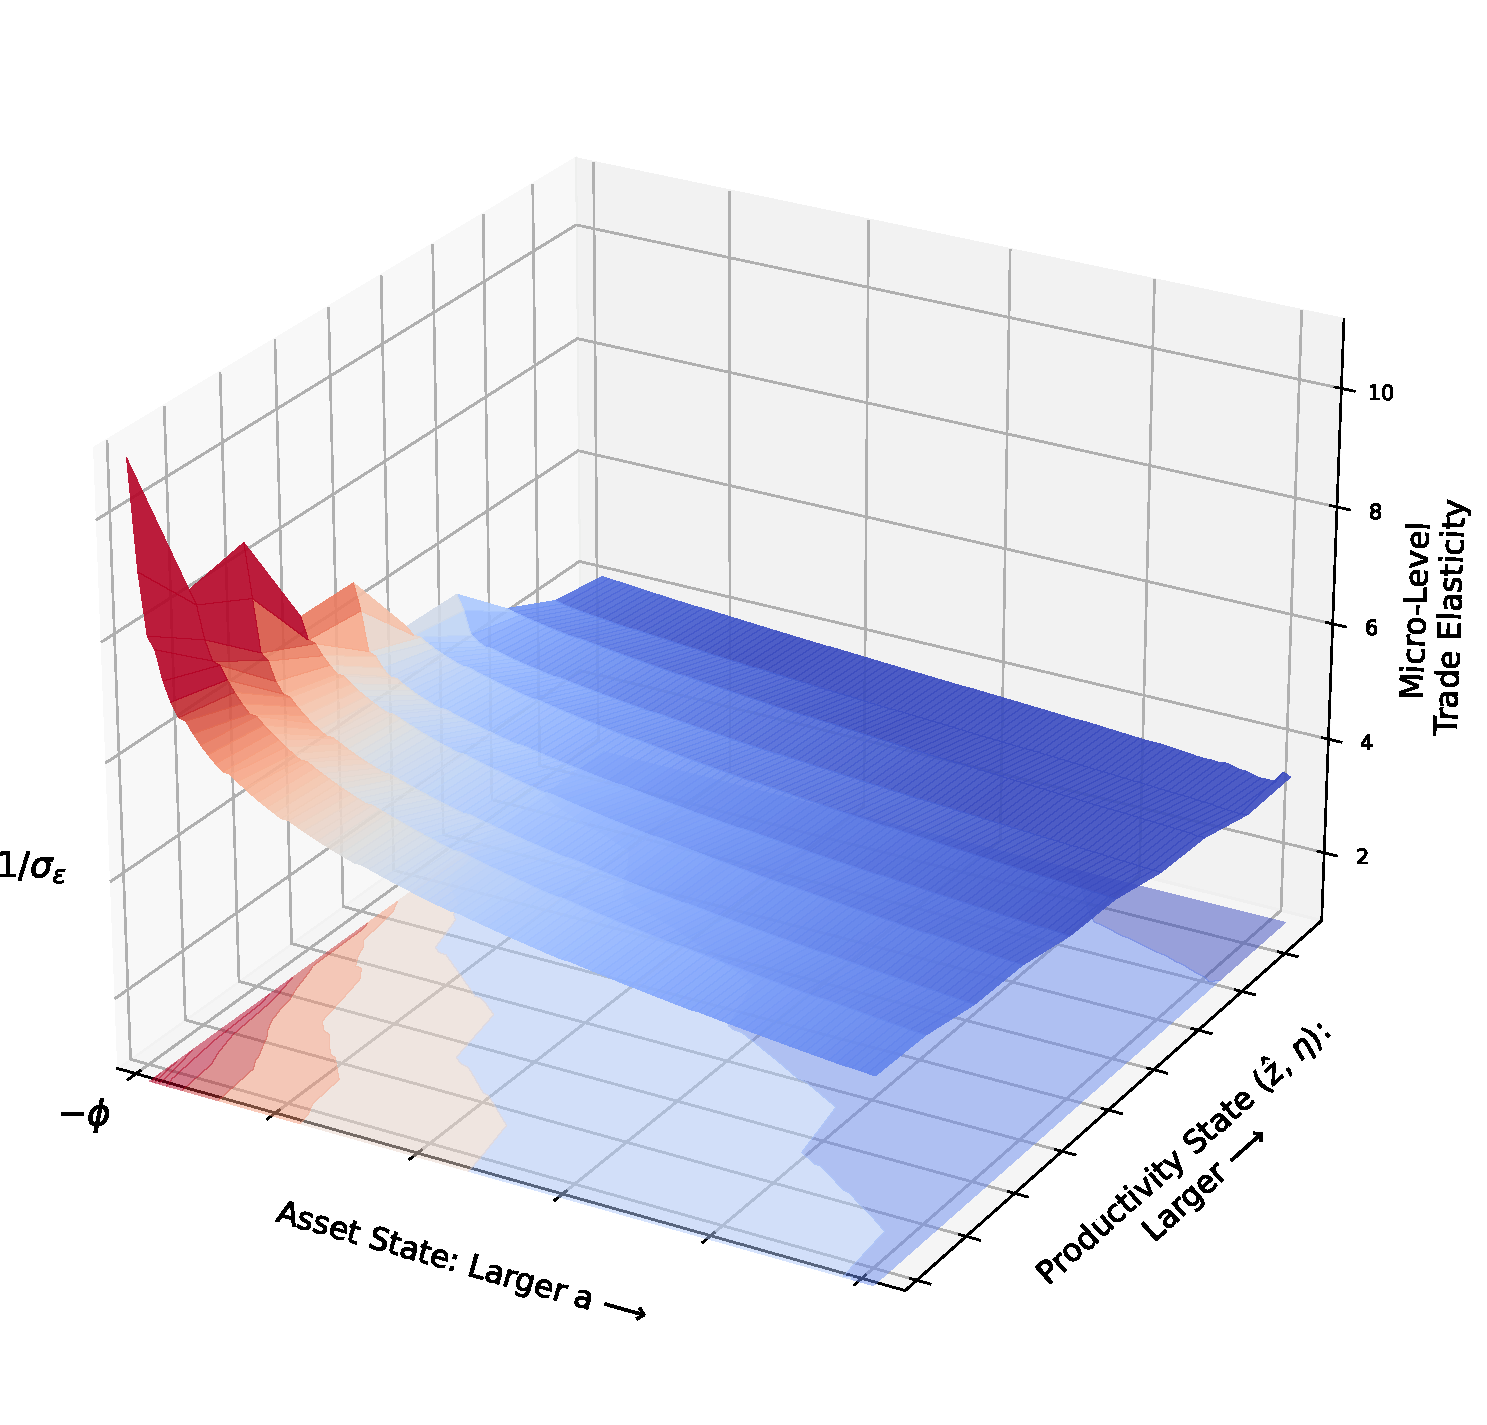
\includegraphics[scale = .37]{./figures/micro-elasticity.pdf}}
\caption{Household-Level Elasticities, $-\theta_{ij}(a,z)$}\label{fig:micro-elasticity}
\end{subfigure}
\begin{subfigure}{.45\textwidth}
\centering
\centering{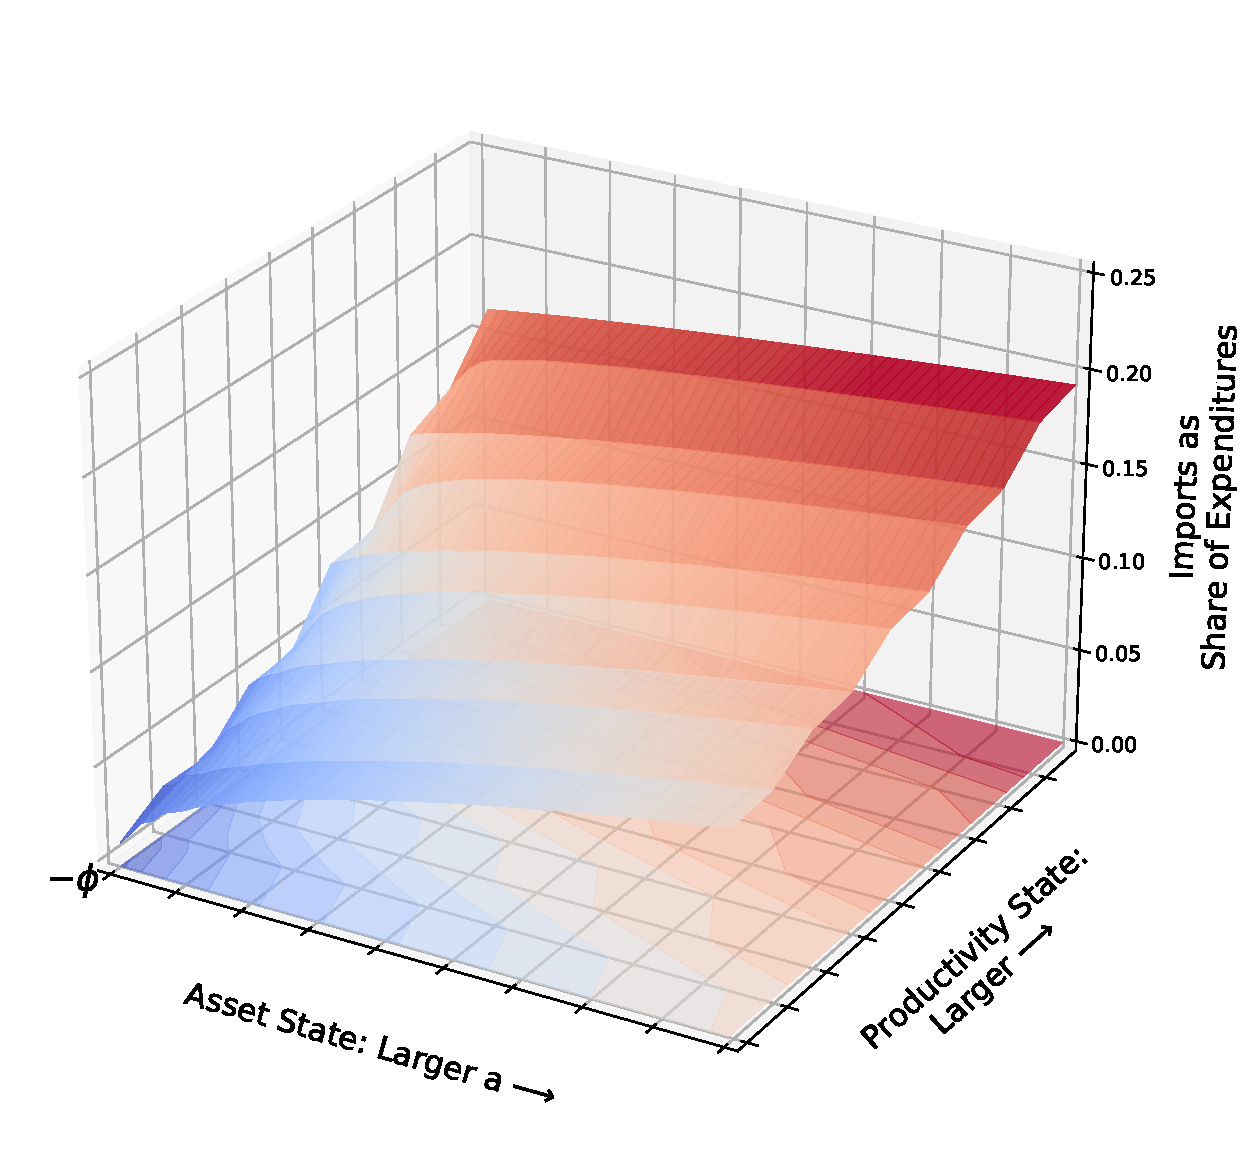
\includegraphics[scale = .37]{./figures/trade-share.pdf}}
\caption{Household-Level Import Shares}\label{fig:micro-trade}
\end{subfigure}
\end{figure}

Figure \ref{fig:micro-elasticity} and \ref{fig:micro-trade} illustrates how this works in a two country economy. Figure \ref{fig:micro-elasticity} plots the absolute value of the trade elasticity (intensive and extensive margin) by household state (assets are on the x-axis, productivity state on the y-axis) and the borrowing constraint $\phi$ is in the south-west corner. This shows is how the trade elasticity systematically varies with assets and income: Poor households|especially those near the borrowing constraint|are very price elastic with a trade elasticity of around $-10$. Richer households are less price elastic with this elasticity declining towards $-3.$

This pattern of trade elasticities has a strong intuitive feel and there is evidence in support of it.\footnote{This idea goes back to \citeapos{harrod1936trade} ``Law of Diminishing Elasticity of Demand'' that says that price sensitivity declines with income which is not to be confused with Marshall's Second Law of Demand which I discuss later.}. This result comes out of estimates in \citet{berry1995automobile} and in a more macro context, \citet{nakamura2010accounting}. \citet{sangani2022markups} is a recent paper that provides evidence in support of this fact from the Kilts-Nielsen data set. The evidence in \citet*{auer2022unequal} most closely relates to the patterns in Figure \ref{fig:micro-elasticity} with poorer households having higher price elasticities; \citet*{colicev2022impact} finds similar results.

One more implication of this result: because rich and poor households face the same prices, differences in elasticities lead to different expenditure shares. Figure \ref{fig:micro-trade} illustrates this point by plotting expenditure on the foreign good relative to total expenditure. Because of trade costs and symmetry across countries, the home good is the relatively cheaper good. Thus, poor, high-price-elastic households spend more on the cheap home good versus the expensive foreign good. In fact, for those near the borrowing constraint in this example, it's near zero.

\subsection{The Gains from Trade}

In this section I compute how social welfare changes due to a change in trade costs. I derive these gains across steady states, the idea here is that I'm thinking a situation where the change is small and there is an immediate jump to the new steady state. The purpose here is to heuristically illustrate mechanics and where the gains from trade arise from. Unlike the trade elasticity, I take total derivatives that encompass general equilibrium changes in wages and interest rates.

The analysis proceeds in several steps before stating the main result in Proposition \ref{prp:gains-trade}. First, I focus only on country $i$ and study a change in trade costs $d_{ij}$. To simplify the algebra, I choose $w_i$ to be the numeraire and normalize $A_i = 1$. This implies is that $p_{ii}$ equals one and it's derivative with respect to a change in trade costs is zero as it's pinned down by my choice of normalizations.

I focus on country $i$ with a utilitarian social welfare function:
\begin{align}
W_{i} = \int_{z} \int_{a}  v_{i}(a,z) L_i \lambda_{i}(a,z)
\label{eq:social-welfare}
\end{align}
where $v_{i}(a,z)$ is a households ex-ante (before preference shocks are realized) value function in country $i$, with states $a,z$. The total change in total welfare is
\begin{align}
\frac{\mathrm{d} W_{i}}{\mathrm{d} d_{ij} / d_{ij}} \approx \int_{z} \int_{a} \bigg \{ \frac{\mathrm{d} v_i(a, z)}{\mathrm{d} d_{ij} / d_{ij}}  + v_{i}(a,z) \frac{\mathrm{d} \lambda_{i}(a,z)/ \lambda_{i}(a,z)}{\mathrm{d} d_{ij} / d_{ij}}  \bigg \} L_i \lambda_{i}(a,z) \ da \ dz.
\label{eq:social-welfare-change}
\end{align}
where the $\approx$ symbol reinforces that this is a heuristic, thinking about a small change and there is an immediate jump to the new steady state.

At a high-level, (\ref{eq:social-welfare-change}) illustrates that the gains from trade come through two forces. The first component reflects changes in household-level welfare. So conditional on a distribution of households across states, this computes if households are better (or worse!) off from the change. Relative to the efficient allocation this force is always present, however, the planner equalizes things across households such that individual states do not matter and, thus, distributional issues do not matter.

The second component of (\ref{eq:social-welfare-change}) is about reallocation. It says: take the old $v$'s and compute how the change in the distribution (that arise because of behavioral responses of households) effects social welfare. So does trade make it more or less likely that households are in ``good'' parts of the distribution. This force is unique to the decentralized allocation and symptomatic of an inefficiency in the initial allocation.

In total, the change in social welfare is then the weighted average of these two forces with the weights being those at the initial distribution.

A key issue is how household-level welfare changes. Here, I make the use of the observation in Equation (\ref{eq:log_sum-home}) that the ex-ante value function can be represented in only in terms of home choice $ii$ values and then recursively push forward. In other words, I can compute $\frac{\mathrm{d} v_i(a, z)}{\mathrm{d} d_{ij} / d_{ij}}$ \emph{as if} one only consumed the home good for the infinite future. This observation gives rise to the following:
\begin{align}
\frac{\mathrm{d} v_i(a, z)}{\mathrm{d} d_{ij} / d_{ij}} =& -\sigma_{\epsilon} \frac{\mathrm{d} \pi_{ii}(a,z) / \pi_{ii}(a,z)}{\mathrm{d}d_{ij} / d_{ij}} \ + \ u'(c_{i}(a,z,i))a \ \frac{\mathrm{d} R_{i}}{\mathrm{d} d_{ij} / d_{ij}} \\
\nonumber \\
& + \beta \mathbb{E} \bigg \{ -\sigma_{\epsilon} \frac{\mathrm{d} \pi_{ii}(a',z') / \pi_{ii}(a',z')}{\mathrm{d}d_{ij} / d_{ij}} +  u'(c_{i}(a',z',i))\frac{\mathrm{d} R_{i}}{\mathrm{d} d_{ij} / d_{ij}}a' \ \  \ldots \mbox{and into the future.} \nonumber
\end{align}
The first term: $-\sigma_{\epsilon} \frac{\mathrm{d} \pi_{ii}(a,z) / \pi_{ii}(a,z)}{\mathrm{d}d_{ij} / d_{ij}}$ is what I'll call \emph{gains from substitution}. The second term is what I'll term as \emph{gains to asset trade}.\footnote{As discussed previously and worked out in the Appendix, the general expression has terms reflecting the effect of borrowing constraints. But again, envelope arguments for small changes mean that these terms are zero.}

Finally, these repeat themselves into the expected future, appropriately discounted. Proposition \ref{prp:gains-trade} summarizes the result below.
\begin{prp}[\textbf{H-A Gains from Trade}] \label{prp:gains-trade} The welfare gains from trade are given by
{\footnotesize
\begin{align}
\frac{\mathrm{d} W_{i}}{\mathrm{d} d_{ij} / d_{ij}} \approx \int_{z} \int_{a}  \bigg \{ \frac{\mathrm{d} v_i(a, z)}{\mathrm{d} d_{ij} / d_{ij}}  + v_{i}(a,z) \frac{\mathrm{d} \lambda_{i}(a,z)/ \lambda_{i}(a,z)}{\mathrm{d} d_{ij} / d_{ij}}  \bigg \} L_i \lambda_{i}(a,z).
\nonumber
\end{align}
}which reflects the change in household level gains and how the distribution of households changes. Household level gains are given by
{\footnotesize
\begin{align}
\nonumber
\frac{\mathrm{d} v_i(a, z)}{\mathrm{d} d_{ij} / d_{ij}} = \mathbb{E}_{z} \sum_{t = 0}^{\infty} \beta^{t} \bigg \{ -\sigma_{\epsilon} \frac{\mathrm{d} \pi_{ii}(a_{t},z_{t}) / \pi_{ii}(a_{t},z_{t})}{\mathrm{d}d_{ij} / d_{ij}} + u'(c_{i}(a_{t},z_{t},i))a_{t} \times \frac{\mathrm{d} R_{i}}{\mathrm{d} d_{ij} / d_{ij}} \bigg \}
\end{align}
}where each term represents:
\begin{itemize}
\item Gains from substitution: $-\sigma_{\epsilon} \frac{\mathrm{d} \pi_{ii}(a_{t},z_{t}) / \pi_{ii}(a_{t},z_{t})}{\mathrm{d}d_{ij} / d_{ij}}$.

\item Gains to asset trade: $u'(c_{i}(a_{t},z_{t}, i))a_{t} \times \frac{\mathrm{d} R_{i}}{\mathrm{d} d_{ij} / d_{ij}}$
\end{itemize}
\end{prp}
Before moving on, I unpack the components in this result and provide some intuition.

\textbf{Gains from substitution.} The change in the home share summarizes two forces: (i) how exposed a household is to the change through the choice probabilities and then (ii) elasticities. To see this, define $\bar{\theta}(a,z) ^E_{ij',j}$ as the extensive margin, cross-price elasticity, in total derivative form (and it's derivation follows what is done in \ref{eq:extensive-margin}). As I show in the Appendix \ref{apx-sec:gains-trade}, the change in the home share can be expressed as:
\begin{align}
-\sigma_{\epsilon} \frac{\mathrm{d} \pi_{ii}(a,z) / \pi_{ii}(a,z) }{\mathrm{d} d_{ij} / d_{ij}} &= \sigma_{\epsilon} \sum_{j'} \pi_{ij'}(a,z) \times \bigg[ \bar{\theta}(a,z) ^E_{ii,j} - \bar{\theta}(a,z) ^E_{ij',j}\bigg], \\
\nonumber \\
&\approx
-\sigma_{\epsilon} \times \pi_{ij}(a,z) \times \bar{\theta}(a,z) ^E_{ij,j}.
\label{eq:gains-substitution}
\end{align}
In words, the top line says that the change in home choice probability is equivalent to a weighted average of relative cross-price elasticities with the weights being the choice probabilities.

The next line assumes that all cross-terms are small, then the gains from substitution depend upon the initial exposure of a household to market $j$ and their own-price elasticity (the total derivative analog to (\ref{eq:extensive-margin}). And because the own-price elasticity is intimately connected to marginal utility of consumption, the elasticity effect picks up the intuitive idea that one aspect of the gains from trade is a household's individual valuation of the price reduction, in addition to the household's exposure.

Equation (\ref{eq:gains-substitution}) is interesting for several reasons. First it is analogous to the gains from trade formula in the efficient allocation (Proposition \ref{prp:gains-efficient-allocation}). The difference is that in that market incompleteness leads to heterogeneity in both exposure \emph{and} elasticities giving rise to heterogenous gains from trade.

This expression also connects with two related papers. \citet{borusyak2021distributional} (following an approach dating back to at least \citet{} consider an environment where, to a first order, only exposure matters, similar to the exposure term in Equation (\ref{eq:gains-substitution}). \citet{auer2022unequal} work out second order effects with non-homothetic CES preferences and additional effects from elasticities show up, similar to the elasticity term in (\ref{eq:gains-substitution}). The interpretation here has a different flavor than articulated in \citet{auer2022unequal}. Because elasticities are intimately connected with the marginal utility of consumption, this relationship is saying that the reason high elasticity households gain (conditional on exposure) more, is because the price reduction from trade is more valuable, on the margin.

\textbf{Gains to asset trade.} The idea here is that changes in trade costs affect the equilibrium interest rate in the country and then benefit (or hurt) households depending upon their net asset position. For example, if a trade liberalization leads to an increase in interest rates, net debtors suffer since their terms to borrow deteriorated, while net savers benefit.

Why might a trade liberalization change interest rates? It's because the liberalization has heterogenous effects on expenditure patterns and savings through the forces discussed in Section \ref{sec:trade-elasticity}. So if the liberalization disproportionately benefits rich /savers in the economy, they shed assets to consume a bit more of the now cheaper goods. Then interest rates must increase to clear financial markets impacting the poor / debtors in the economy. The novelty here is how the goods trade and the financial market are interlinked|not separate as they are typically treated.

\subsection{Elasticities and Gains in the Efficient Allocation}\label{sec:log-preferences}

One issue behind the results above is market incompleteness. Households are imperfectly insured against the risks they face, this leads to heterogeneity in the marginal utility of consumption and, in turn, heterogeneity in price sensitivity, expenditure patterns, and the gains from trade. This section contrasts these previous results with an allocation where a social planner can overcome market incompleteness and, thus, I shed some light on what role market incompleteness is playing in the analysis.

The starting point is a utilitarian social welfare function:
\begin{align}
W = \sum_{i} \underbrace{\sum_{t=0}^{\infty} \int\limits_{z} \beta^{t}  v_{i}(z,t) L_{i}\lambda_{i}(z,t)}_{W_i},
\label{eq:planner-welfare}
\end{align}
and here $v_i(z,t)$ is a households ex-ante utility with state $z$, time $t$, in country $i$. I highlight the under-braced term $W_i$ as the welfare of those living in country $i$ and which is analogous to (\ref{eq:social-welfare}).

In \citet{waughoptimal}, I fully characterize a Planner's choice of consumption allocations $c_{i}(z, j, t)$ and choice probabilities $\pi_{ij}(z,t)$ for all $i,j$ pairs, $z$ states, and dates $t$ to maximize (\ref{eq:planner-welfare}). Given a characterization of the optimal allocation, I can compute the welfare gains from a change in trade costs and study how welfare changes across the two stationary allocations.\footnote{Unlike the previous section, the move across stationary allocations is no consequence as there is no moving aggregate state variable, so the jump across stationary equilibrium is instantaneous.}

Proposition \ref{prp:gains-efficient-allocation} describes the result, Appendix \ref{sec:apx-planner} works out the details.

\begin{prp}[\textbf{Trade Elasticities and Welfare Gains in the Efficient Allocation}]\label{prp:gains-efficient-allocation} The elasticity of trade to a change in trade costs between $i,j$ in the efficient allocation is:
\begin{align}
\theta_{ij} =  -\frac{1}{\sigma_{\epsilon}} \bigg [ u'(c_{i}(j)) c_{i}(j) \bigg]. \label{eq:eff-trade-elasticity}
\end{align}
And the welfare gains from a reduction in trade costs between $i,j$ are
\begin{align}
\frac{\mathrm{d} W}{\mathrm{d} d_{ij} / d_{ij}} = \frac{\partial W}{\partial d_{ij} / d_{ij}} = \frac{\sigma_{\epsilon} \  \theta_{ij} \  \pi_{ij} \ L_i}{1-\beta}
\label{eq:eff-trade-gains}
\end{align}
which is the discounted, direct effect from relaxing the aggregate resource constraint.
\end{prp}
Proposition \ref{prp:gains-efficient-allocation} highlights a couple of things. First, the trade elasticity is both similar and different than typically thought. Consistent with intuition from \citeapos{eaton2002technology}, the dispersion parameter matters inversely. If $\sigma_{\epsilon}$ is small, national varieties are ``as if they are near substitutes'' and thus trade flows will respond a lot.

The non-standard part of the trade elasticity is that the marginal utility of consumption times consumption shows up. One way to view this part of the elasticity is that it's the rate of conversion from quantities into utils. That is how many utils, on the margin, a particular quantity of level of consumption delivers. And this matters for the elasticity in a very intuitive way|country pairs that deliver a lot of utility, on the margin, are the pairs where the planner will be most responsive to changes in trade costs.

The second part of Proposition \ref{prp:gains-efficient-allocation} summarizes the gains from trade. It says that the total change in welfare only reflects those eating that commodity $\pi_{ij} \times L_i$ which is the share of households consuming commodity $j$ times the number of households in country $i$. This is then converted into utils using the elasticity which, as discussed above, is something about the dispersion in shocks and then the rate at which utils are being delivered at current quantities.\footnote{An alternative perspective is to divide through both sides of (\ref{eq:eff-trade-gains}) by the marginal utility of consumption and then the welfare is in money metric units.} This is then discounted for the infinite future, hence the $1/ (1-\beta)$ term.

This is just the direct effect from a reduction in trade costs relaxing the resource constraint and converted to utils appropriately. Behind this result is an envelope-type argument with direct effects only mattering because I'm evaluating the change in welfare at the optimized allocation and any benefits of adjusting consumption and choice probabilities are zero|on the margin.

This result is reminiscent of \citet{AtkesonBurstein2010} who make a similar claim in the context of a model with rich firm heterogeneity. They show that the only first order effect of lower trade costs on welfare is the direct consumption effect and that indirect effects are second order. This is similar, but with household heterogeneity, by saying that, in the efficient allocation all margins are properly equated heterogeneity is irrelevant and the welfare gains only the direct benefits.

Before moving on, let me connect the results in Proposition \ref{prp:gains-efficient-allocation} with \citet{arkolakis2012new}. As I show in the appendix, in the efficient allocation the percent change in the home choice probability exactly equals the $i, j$ choice probability times the trade elasticity
\begin{align}
\frac{\mathrm{d} \pi_{ii} / \pi_{ii}}{\mathrm{d} d_{ij} / d_{ij}} = -\theta_{ij} \times \pi_{ij},
\label{eq:effecient-home-share}
\end{align}
then inserting (\ref{eq:effecient-home-share}) into  (\ref{eq:eff-trade-gains}) I have
\begin{align}
\frac{\mathrm{d} W}{\mathrm{d} d_{ij} / d_{ij}} =  \sigma_{\epsilon} \times \frac{\mathrm{d} \pi_{ii} / \pi_{ii}}{\mathrm{d} d_{ij} / d_{ij}} \times \frac{L_i}{1 - \beta}.
\label{eq:eff-trade-gains}
\end{align}
Now the form of (\ref{eq:eff-trade-gains}) is closely related to \citet{arkolakis2012new}. Interestingly, and much like in the decentralized allocation, the change in the home choice probability summarizes a lot. Moreover, now there is an equivalence between \citet{AtkesonBurstein2010}-like logic and \citet{arkolakis2012new}-style formulas.

There are two details: choice probabilities do not necessarily correspond with expenditure shares and the $\sigma_{\epsilon}$ is not the inverse of the trade. However, with $\log$ the trade elasticity becomes $1 / \sigma_{\epsilon}$, choice probabilities are proportional to expenditure shares, and the correspondence between the gains from trade under efficiency and \citet{arkolakis2012new} becomes exact. The case of $\log$ has an additional implication that heterogeneity and market incompleteness does not matter for trade outcomes and I turn to this case next.

\subsection{The Case of $\log$ preferences}\label{sec:log-preferences}

The case of $\log$ preferences over the physical commodity displays some unique features. This (very common) preference structure leads to an interesting result where micro-level heterogeneity, market incompleteness completely sperate from the trade side of the economy. So in this one case, trade behaves ``as if'' there were a representative agent Armington-CES consumer and then the gains from trade take the form in \citet{arkolakis2012new}|even though individual households are facing shocks, borrowing constraints, and in general trying to deal with life's circumstances.

Consider the following preference structure:
\begin{align}
\tilde{u}( c_{ij,t} ) =  \log(c_{ij,t}) + \epsilon_{j,t}. \nonumber
\end{align}
There is essentially one insight and then everything follows. Examining the problem in (\ref{eq:value_fun_option}) and substituting in the households budget constraint from (\ref{eq:trade-budget-constraint}), then leads to the observation that the optimal $a'$ conditional on a choice $j$ is \textbf{independent} of the price and the choice $j$. In Appendix \ref{apx-sec:log-preferences}, I employ a formal ``guess and verify'' approach off the Euler equation and show it leads to the same conclusion and this is verified on the computer as well.

Everything follows from this observation.

Because assets don't adjust to changes in prices, from (\ref{eq:intensive-margin}) the intensive margin elasticity for $ij$ is minus one. On the extensive margin, things are more involved as at the micro level they are varying by income and assets. But across different destinations, within states, they vary in the same exact way. Given that the trade elasticity is always defined relative to home choices, heterogenous effects wash out and the end result is that everything collapses to $-\frac{1}{\sigma_{\epsilon}}$. Similarly, aggregate trade satisfies a gravity-like relationship (which no role for household heterogeneity) as in a CES-Armington model or \citet{eaton2002technology}.

Working from Proposition \ref{prp:gains-trade} one can see how the gains only depend on aggregates. The reallocation term in (\ref{eq:social-welfare-change}) is zero because asset holdings don't change. The gains to asset trade are zero because $R$ does not move. Thus, the gains from trade are only about the discounted stream of changes in the home choice probability $\pi_{ii}$|which is the same for rich and poor households per the argument in the previous paragraph.

Appendix \ref{apx-sec:log-preferences} works through this logic step-by-step. Below I state the result:
\begin{corr}[\textbf{Separation of Trade and Micro-Heterogeneity}]\label{prp:seperation} In the dynamic, heterogenous agent trade model where preferences are logarithmic over the physical commodity: The trade elasticity is
\begin{align}
\theta = -\frac{1}{\sigma_{\epsilon}}, \nonumber
\end{align}
and relative trade flows satisfy a gravity relationship
\begin{align}
\frac{M_{ij}}{M_{ii}} = \left( \frac{  w_{j} / A_{j} }{  w_{i} / A_{i} } \right)^{\frac{-1}{\sigma_{\epsilon}}} d_{ij}^{\frac{-1}{\sigma_{\epsilon}}}, \nonumber
\end{align}
and are independent of the household heterogeneity. Ant the welfare gains from trade are
\begin{align}
\frac{\mathrm{d} W_{i}}{\mathrm{d} d_{ij} / d_{ij}} = -\frac{1}{\theta (1-\beta)} \times \frac{\mathrm{d} \pi_{ii} / \pi_{ii}}{\mathrm{d}d_{ij} / d_{ij}}. \nonumber
\end{align}
and is (i) independent of the household heterogeneity and (ii) summarized by the trade elasticity and the change in the home choice probability.
\end{corr}
To be honest, I found this result surprising. By looking at the choice probabilities in (\ref{eq:choice-prob}) and noting how the value functions determine choices, not period utility functions, one would suspect that the household's income fluctuations problem would shape aggregate trade outcomes. Corollary \ref{prp:seperation} shows that is not the case but that micro-outcomes and aggregate trade outcomes ``separate.''

Not only does heterogeneity not matter, aggregate outcomes essentially mimic the results of \citet{arkolakis2012new} and, thus, my heterogenous agent model \emph{with log preferences} delivers the ``same old gains.'' Trade flows take a constant elasticity form with the trade elasticity pinned down by the dispersion parameter on the trade shocks. And then the total change in welfare is summarized by the trade elasticity and how the share of home purchases changes to any change in trade costs.

Proposition \ref{prp:seperation} is also interesting because it generalizes the results of \citet*{anderson1987ces} and \citet{anderson1992discrete} to a far more complicated economy. They showed that in a static model with log utility and additive logit shocks, the economy behaves \emph{as if} there were a representative agent CES consumer. I recover their result, but I must emphasize the complexity of the economy at the micro-level for which this result stands|households are froward looking, face productivity and taste shocks in the presence of incomplete markets and borrowing constraints. Yet, these details don't matter when the magic of $\log$ kicks in.

\section{Calibration}

This section focuses on my approach to calibrating the model. The next two subsections discuss the preference specification, income and taste shock process, borrowing constraints and how I scale things so the model can deliver balanced growth like properties.

The final section follows the trade literature by picking country specific TFP and trade cost parameters to match bilateral trade flows. How I do this is a novelty | I use ``gravity as a guide'' to overcome the fact that my model does not admit a closed form map from trade flows to parameters as static, gravity models do. I describe this approach below and then discuss how the remaining non-country specific parameters are chosen.

\subsection{Functional Forms, Quality Shifters, Balanced Growth Scaling}

Utility over the physical commodity is CRRA with relative risk aversion $\gamma$. On top of these preferences I do several things to ensure that micro and macro facts can be matched given that there is a sense in which preferences are non-homothetic on the extensive margin.

The first feature I introduce are household-specific quality shifters. This is important because it helps the model match facts regarding how import shares vary across rich and poor households (see, e.g., \citet{borusyak2021distributional}). The necessity of quality shifters relates to the discussion around Figure \ref{fig:micro-trade} | that prices and price elasticities determine how shares vary across households and these forces lead to a pattern of sorting with poor, high-elasticity households concentrating their expenditures on the cheapest commodities available. Quality shifters that vary with household-specific characteristics are one way to match shares, yet allow for heterogeneity in price elasticities. \citet{berry1995automobile} make this point and it motivates their modeling of demand with interactions between attributes of the product and household characteristics; \citet{auer2022unequal} allows for this force as well in both their model and empirical specification.

Mechanically, I implement quality shifters by introducing a home bias term $\psi_{ii}(z)$ which additively shifts period utility when consuming the home good $i$ and it is indexed by the households productivity state $z$. This last point implies that rich and poor households may have different valuations quality between home and foreign goods. To reduce $\psi$s dimensionality, I assume that it's a log-linear function of a households permanent productivity state and this function is the same across countries. The slope of this relationship is calibrated to match the fact from \citet{borusyak2021distributional}) that import expenditure shares are essentially the same between US poor (below median income) and rich (above median income) households.

The second feature is that I want things to scale and deliver a ``balanced-growth-like'' property. Specifically, the want-operator here is that if there were two countries one with high TFP and one with low TFP, elasticities (both at the micro and macro level) in the two countries are the same. The way to do this is to make the Type 1 Extreme value parameter country specific and scaled so that $\sigma_{\epsilon,i} = \sigma_{\epsilon} A_i^{1-\gamma}$ and similarly for the quality shifters above.

\subsection{Shocks and Constraints}

The income shock process is set up to be a mixture of a AR(1) persistent component and an iid transitory component and this is calibrated using results from \citet*{krueger2016macroeconomics}. I use their exact parameter values. It is assumed to be the same across countries.

The borrowing constraint is set in the following way. First, I scale it by a country's autarky level of average real labor income. Then it is set so that a household can borrow up to fifty percent of it's autarky level of income. The scaling here is done to deliver a balanced-growth-like property of the model so a households debt capacity is invariant to a country's autarky level of income.

In my main calibration, I work with the case of financial globalization. In this case there is one interest rate clearing the global asset market. All countries are assumed to have the same discount factor and it is set so the equilibrium world interest rate is 1 percent.

Per the discussion above, the taste shock parameter is set in the following way. TFP in the United States is normalized to one and then, per the discussion above, I set this so that $1 / \sigma_{\epsilon} = 4.0$ and, thus, $1 / \sigma_{\epsilon,us} = 4.0$. And again, per the discussion above, all other countries shock parameters are pinned down by $\sigma_{\epsilon}$ and their level of TFP $A_i$.



\subsection{Using Gravity as a Guide to Match Trade Data}

My calibration strategy is to use the gravity regression as a guide in an indirect inference procedure where I estimate parameters of the model so that the regression coefficients from a standard gravity regression run on my model's data match the coefficients when the same regression is ran on the data.

Here are the details. The bilateral trade flows that I use are from \citet{eaton2002technology}. The 19 countries in this data set is a nice size to do what I want to do in about an afternoon. Moreover, the \citet{eaton2002technology} data set provides a well defined benchmark disciplined by bilateral trade flows and gravity variables.

In the 19 country model, the parameters I need to choose are $19 - 1$ country-specific TFP parameters (the $A_i$s) and then $(19-1) \times (19-1)$ trade costs (with the minus one since the $ii$ trade costs is normalized to one) to infer from the bilateral trade data. This leaves me under-identified with  only $(19-1) \times (19-1)$ bilateral trade shares and $19 -1$ TFP parameters.

\textbf{Step 0.} I'll reduce the number of parameters to estimate by placing a restriction on trade costs that are a function of observable data. Specifically, I assume that trade costs take the form as in \citet{eaton2002technology} with
\begin{align}
\log d_{ij} = d_{k} + b + l + e_{h} + m_{i},
\label{eq:trade-cost-function}
\end{align}
where trade costs are a logarithmic function of distance, where $d_k$ with $k = 1,2,...,6$, is the effect of distance between country $i$ and $j$ lying in the $k$-th distance interval.\footnote{Intervals are in miles: $[0,375)$; $[375,750)$; $[750,1500)$; $[1500,3000)$; $[3000,6000)$; and $[6000,\mbox{maximum}]$. } The $b$ term is the effect of a shared border in which $b =1$ if country $i$ and $j$ share a border and zero otherwise. Similarly $l$ is a dummy variable if country's $i$ and $j$ share a language, and $e_{h}$ represent two dummy variable for different indicators of European integration. The final part is an importer fixed effect shifting trade costs up or down depending upon the identity of the importer.

At this point, I've reduced the parameter space to the  coefficients on the trade cost function rather than the complete matrix of trade costs and then the TFP terms.

\textbf{Step 1.} The next step is to run the following gravity regression on the data
\begin{align}
\log \left( {\frac{M_{ij}}{M_{ii}}} \right) = {im_{i}} + {ex_{j}} + {d_{k}} + {b} + {l} + {e_{h}} + \delta_{ij},
\label{eq:gravity-data}
\end{align}
which projects imports between country $i$ and $j$ ( normalized relative to domestic expenditures ) on an importer effect, exporter effect and then the gravity variables relating to distance, border, language, etc. and finally there is an error term $\delta_{ij}$ that reflects other factors not in this specification.

This is the canonical representation of trade flows|the gravity model. In a standard Armington-CES, \citet{eaton2002technology}, or \citet{melitz2003impact} style model, the importer effects and exporter effects have specific interpretations. And given the point estimates from (\ref{eq:gravity-data}), productivity and the importer fixed effects on the trade cost function are easily recovered.

In my model, this is not the case. However, the idea is to use the point estimates from (\ref{eq:gravity-data}) as moments for my model to match. The next step constructs model analogs to (\ref{eq:gravity-data}).
%
%Abstracting from normalizations, I now have $19 + 29$ point estimates to match up with the $19 + 29$ parameters I need to estimate.\footnote{To be clear about normalizations: I really only have 18 TFP parameters to match and then a normalization on the importer fixed effects is that they sum to zero as in \citet{eaton2002technology}. The fixed effects in \ref{eq:gravity-data} satisfy the normalization that each of their sum is zero. Thus I have $18 + 28$ parameters to match $18 + 28$ moments}

\textbf{Step 2.} To construct model analogs to (\ref{eq:gravity-data}), I guess TFP parameters and coefficients on the trade cost function in (\ref{eq:trade-cost-function}). Define this parameter vector as $\Theta$.

Given $\Theta$, I compute an equilibrium of the world economy. This amounts to: (i) solving for households' dynamic problems|in each country (ii) constructing the stationary distribution of wealth and expenditure patterns|in each country (iii) aggregating and then (iv) finding a vector of prices so goods markets and financial markets clear world wide.

Once I find an equilibrium, I run the same regression as in (\ref{eq:gravity-data}) on the model generated data. As some notation, the model constructed moments are defined as, e.g., $im_{i}(\Theta)$ which is the importer effect estimated on model generated data under the parameter vector $\Theta$.

\textbf{Step 3.} The final step constructs moment conditions which provide the foundation for estimation. Define $\mathbf{y}(\Theta)$ as a set of moments conditions comparing the point estimates from the data with the point estimates from the model under the parameter vector $\Theta$. For example, ${im_{i}} - im_{i}(\Theta)$ or $d_k - d_k(\Theta)$, etc.

My estimation procedure is based on the moment condition
\begin{align}
E\left[\mathbf{y}(\Theta_o)\right] = 0,
\end{align}
where $\Theta_o$ is the true value of $\Theta$. Thus, my method of moments estimator is:
\begin{align}
\hat{\Theta} = \arg\min_{\Theta} \left[\mathbf{y}(\Theta)'\ \mathbf{y}(\Theta)\right], \label{eq:smm-condition}
\end{align}
At a mechanical level, finding the minimum to (\ref{eq:smm-condition}) amounts to returning to \textbf{Step 2.} each time and smartly updating parameter guess for $\Theta$. One of the nice features of this set-up and the dimensionality reduction that I did, is that now this is an exactly identified problem and standard root-finding techniques can be applied to update $\Theta$ and a minimum found.

\subsection{Calibration Results}


\begin{table}[t]
\small
\begin{center}
\refstepcounter{table}
\setlength {\tabcolsep}{5.5mm}
\renewcommand{\arraystretch}{1.60}\label{tb-calibration}
\begin{tabular}[t]{l c l}
\multicolumn{3}{c}{{\normalsize\textbf{Table \ref{tb-calibration}: Preferences, Shocks, and Constraints | Calibrated Parameters}} }
\\\hline \hline
Description & Value & \multicolumn{1}{c}{Target}\\
\cmidrule(lr){1-1} \cmidrule(lr){2-2} \cmidrule(lr){3-3}
Discount Factor, \ $\beta$                          & $0.92$ & Global Interest Rate of $1\%$ \\
CRRA parameter, \ $\gamma$                          & $1.50$ & Micro elasticities of \citet{auer2022unequal} \\
Slope of Quality Shifter, \ $\psi_{ii}(z)$          & $0.60$ & Micro import share facts of \citet{borusyak2021distributional} \\
Type One E-V parameter, \ $1 / \sigma_{\epsilon}$    & $4.0$ & --- \\
Borrowing Constraint \ $\phi_{i}$                   & --- & $50\%$ of $i$'s autarky labor income \\
Income Process on \ $z$                             & --- & \citet{krueger2016macroeconomics} \\
\hline
\end{tabular}
\\[0.5ex]
%\parbox{5.95in}{\footnotesize \textbf{Note:} }
\end{center}
\end{table}

\subsubsection{Micro Expenditure Shares, Elasticities, and MPCs}

Table \ref{tb-micro-shares} reports household-level expenditure patterns, trade elasticities, and marginal propensities to consume (MPC). I focus on households in US and I brake down the statistics by household income.\footnote{In the model, my income measure is labor income | income including asset payments or expenditures deliver similar results since all three are highly correlated.}

The first column of Table \ref{tb-micro-shares} \ref{tb-micro-shares} reports the share of imports out of total expenditure for households below median income (poor), at the median, and above the median (rich). An outcome is that the model replicates \citet{borusyak2021distributional} facts that import expenditure shares are the same between US poor (below median income) and rich (above median income) households. As discussed above, a key force behind this result are household-specific quality shifters with poor households having stronger perceived quality of imported goods than rich households.

The second column of \ref{tb-micro-shares} reports household-level trade elasticities. These are constructed at the micro-level as in Proposition \ref{prp:GET} for each type of household and import partner. The import partner elasticities are then aggregated into one number using the household's expenditure weights.

Table \ref{tb-micro-shares} illustrates how price elasticities systematical fall with income. For the poor households with income below the median, elasticities are a bit above 6; for the richest households they are a bit below 4. The middle row reports the elasticity for a household in the middle of the distribution and this is 4.8.  \citet{auer2022unequal} report price elasticities for the median and at points above and below in the income distribution. Similar to Table  \ref{tb-micro-shares}, they find that the household in the middle of the income distribution has an elasticity of 4.8 and those at the top and bottom (which are more extreme points than what I report here) they have elasticities of 3.0 and 6.6. Thus, the elasticities in my model at the micro-level are quantitatively consistent with those found in \citet{auer2022unequal}.

\begin{table}[t]
\small
\begin{center}
\refstepcounter{table}
\setlength {\tabcolsep}{5.5mm}
\renewcommand{\arraystretch}{1.60}\label{tb-micro-shares}
\begin{tabular}[t]{l c c c}
\multicolumn{4}{c}{{\normalsize\textbf{Table \ref{tb-micro-shares}: Model: Shares, Elasticities, and MPCs by Income of US Households}} }
\\\hline \hline
& Import Shares & Trade Elasticities & MPCs\\
\cmidrule(lr){2-2} \cmidrule(lr){3-3} \cmidrule(lr){4-4}
Below Median Income & $0.08$ & $-6.24$ & 0.50\\
Median   & $0.08$ & $-4.88$ & 0.28\\
Above Median Income & $0.08$ & $-3.97$ & 0.17\\
\hline
\end{tabular}
\\[0.5ex]
%\parbox{5.95in}{\footnotesize \textbf{Note:} }
\end{center}
\end{table}

The final column in Table \ref{tb-micro-shares} reports marginal propensities to consume in the model. Recalling the discussion in Section \ref{sec:trade-elasticity} | how trade elasticities vary across households relates to MPCs in equation (\ref{eq:elasticity-mpc}).  MPCs in the model are computed by endowing households a one time, unanticipated cash transfer of 1,000 USD and then computing how consumption changes relative to the transfer. As with the elasticities, household level MPCs are aggregated across the different consumption baskets by the household's expenditure weights.

MPCs are right in the ballpark of what is typically thought plausible with the median annual MPC being a little under 0.30 implying that a household spends about 30 cents per dollar of transfer on consumption; see, e.g., \citet{kaplan2022marginal}.\footnote{With that said, this calibration achieves high MPCs essentially by having very little wealth in the economy. This model feature is consistent with the small quantity of liquid wealth observed in the US economy, but leaves out large amounts of illiquid wealth.} Not surprisingly, poorer households have substantially higher MPCs and richer households lower. And together with the second column, Table \ref{tb-micro-shares} confirms the connection between how sensitive a household is to prices and how sensitive a household is to cash transfers.

To summarize, the model is quantitatively matching salient facts about (i) similar import expenditure shares between rich and poor households as in \citet{borusyak2021distributional}), that (ii) poor households have higher price elasticities relative to rich households as in \citet{auer2022unequal}, and (iii) is able to mimic patterns of marginal propensities to consume as seen in micro data and surveyed \citet{kaplan2022marginal}.

\subsubsection{Aggregate Trade and Trade Elasticities}

\begin{figure}[!t]
\centering{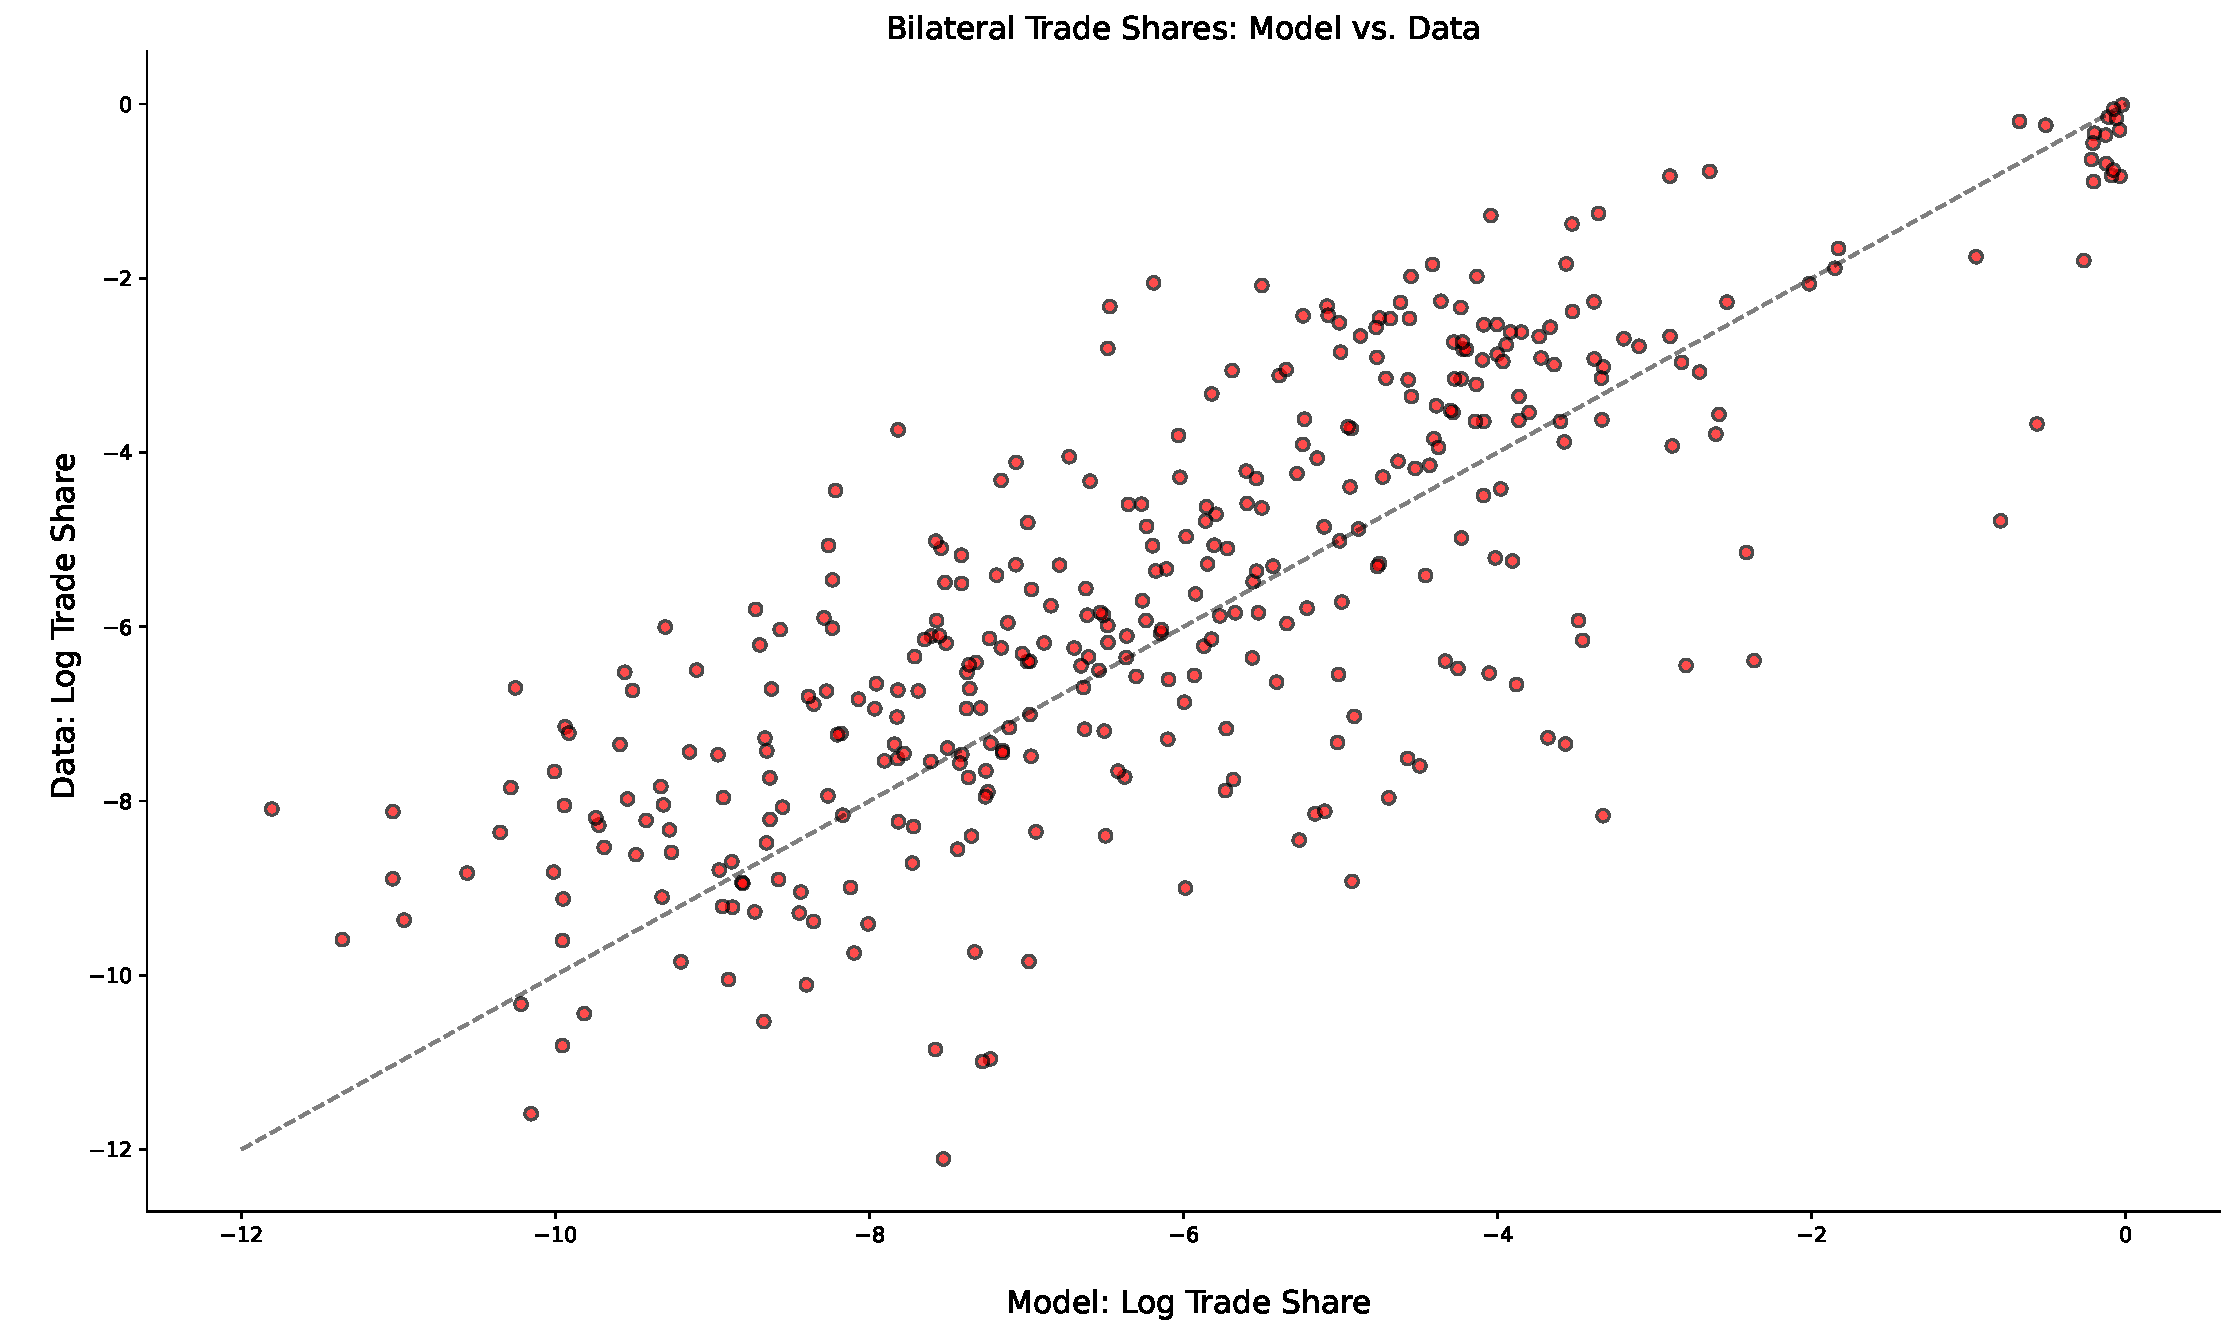
\includegraphics[scale = .45]{./figures/trade-fit.pdf}}
\caption{Bilateral Trade: Model vs. Data}\label{fig:model-fit}
\end{figure}

Figure \ref{fig:model-fit} provides a sense of model fit after running my ``gravity as guide procedure.'' The y-axis reports bilateral trade data and the x-axis reports the outcome from my model. The fit is very high, and nearly indistinguishable from, for example, how a standard trade model perform would perform. Or the $\log$ preference model which per Proposition \ref{prp:seperation} should (and it does) operate just like a standard trade model.

Table \ref{tb-grav-est} reports another measure of fit and some of the resulting parameter values. The first column are the distance, border, etc. moments from the gravity regression in (\ref{eq:gravity-data}) (and note they exactly correspond with those in the top panel of Table 3 of \citet{eaton2002technology}). The second column reports the moments from the model. Here they exactly line up and are consistent with the argument in Figure \ref{fig:model-fit}, the fit is good and the model is replicating geographic pattern of activity seen in the data.

\begin{table}[t]
\small
\begin{center}
\refstepcounter{table}
\setlength {\tabcolsep}{5.5mm}
\renewcommand{\arraystretch}{1.50}\label{tb-grav-est}
\begin{tabular}[t]{l c c c}
\multicolumn{4}{c}{{\normalsize\textbf{Table \ref{tb-grav-est}: Estimation Results}} }
\\\hline \hline
& & \multicolumn{2}{c}{\textbf{HAT-Model}}  \\
\cmidrule(lr){3-4}
Barrier& Moment & Model Fit & Parameter \\
\hline $[0,375)$                &$-3.10 $           & $-3.10 $              & $2.35$           \\
$[375,750)$                     &$-3.67 $           & $-3.67 $              & $2.81$           \\
$[750,1500)$                    &$-4.03 $           & $-4.03 $              & $3.09$           \\
$[1500,3000)$                   &$-4.22 $           & $-4.22 $              & $3.23$           \\
$[3000,6000)$                   &$-6.06 $           & $-6.06 $              & $4.88$           \\
$[6000,\mbox{maximum}]$         &$-6.56 $           & $-6.56 $              & $5.69$           \\
Shared border                   &$\phantom{-}0.30$  & $\phantom{-}0.30$     & $0.91$  \\
Language                        &$\phantom{-}0.51$  & $\phantom{-}0.51$     & $0.87$  \\
EFTA                            &$\phantom{-}0.04$  & $\phantom{-}0.04$     & $0.98$  \\
European Community              &$\phantom{-}0.54$  & $\phantom{-}0.54$     & $0.89$  \\
\hline
\end{tabular}
\\[0.5ex]
\parbox{5.0in}{\footnotesize \textbf{Note:} The first column reports data moments the HAT-model targets. The second reports the model moments. The third column reports the estimated parameter values.}
\end{center}
\end{table}

The final column reports the primitive estimates on the trade cost function. Each value reports the level effect of being in a distance bin or sharing a border etc.  So if two countries are measured to be in the smallest distance bin and share a border, the trade cost between these two countries is $2.35 \times 0.91$ (first row times seventh row). Or if a country is in the furthest distance bin, its trade costs is 5.69.

How would this compare to a standard model? It's a bit hard since one needs to take a stand on the trade elasticity in the standard model to translate estimates in column one into levels of the trade costs. But an approach is the following: find the trade elasticity so the cost of the nearest distance bin is the same as in my model and then look at how things relate in other bins. In an \citet{eaton2002technology} world, this would correspond with an trade elasticity of about 3.6. Then, for example, one takes the moment in the first column, last distance bin and compares $\exp( - 1 / 3.6 \times  -6.56)$ vs. 5.69.

What comes out of is that closer relationship are a bit more expensive then what a constant elasticity model would predict. And the furthest destinations are meaningfully less expensive, seven and ten percent less, for the last two distance bins. This is picking up a model outcome where trade elasticities are increasing with cost. So far away destinations are relatively elastic destinations, so the cost need not be as large to deter trade.

Figure \ref{fig:bilateral-elasticities} provides an example of the of trade elasticities that come of this model. In this figure, I focus on the US and plot each bilateral trade elasticity versus the price a consumer in the US faces when importing a variety from that country. The balls represent the relative size of US imports from that destination. And these elasticities are constructed from the bottom up via the formula in (\ref{eq:trade-elasticity}).

The feature that stands out very clearly in Figure \ref{fig:bilateral-elasticities} is that trade elasticities systematically increase with price and decrease with the volume of trade.

\begin{figure}[!t]
\centering{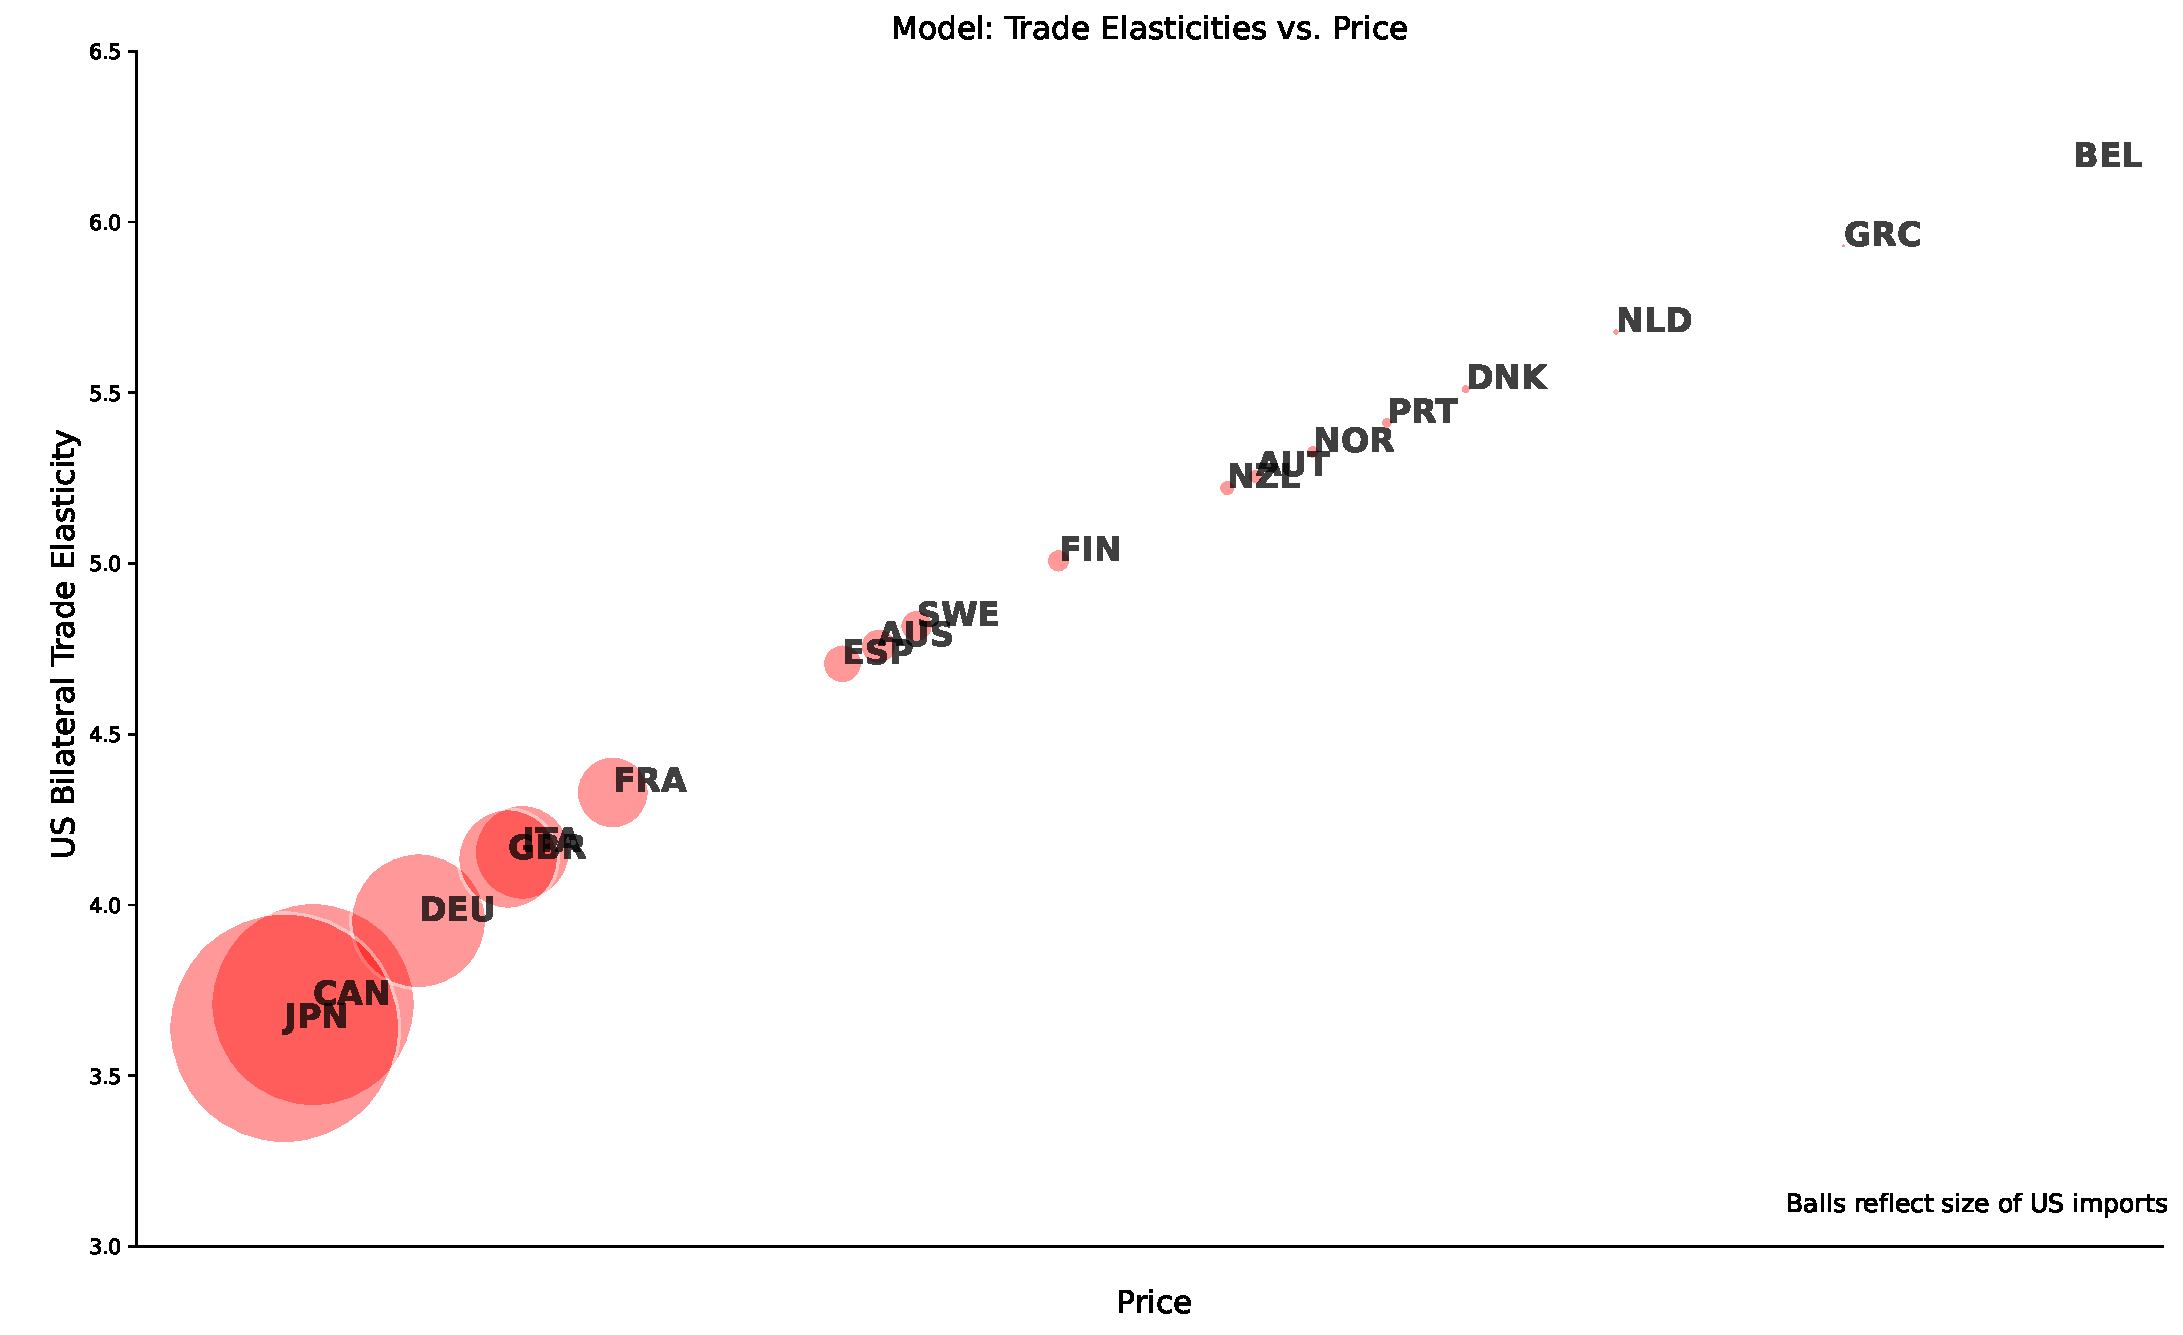
\includegraphics[scale = .45]{./figures/us-elasticity.pdf}}
\caption{Trade Elasticities $-\theta_{us,j}$}\label{fig:bilateral-elasticities}
\end{figure}


At the micro-level, there are two opposing forces giving rise to this aggregate relationship. Per the arguments discussed above around Proposition \ref{prp:GET}, the aggregate bilateral trade elasticity reflects both household level elasticities $\theta(a,z)$s and a composition effect that works through the expenditure weights $\omega(a,z)$s. Thus, when prices increase as one moves from one source to a less competitive source, there are two competing forces at work: (i) how do micro-level elasticities change and (ii) how does composition change?

The first force is that as prices increase \emph{both} rich and poor households' elasticities increase. In other words, everyone is more elastic when contemplating a purchase from a more expensive destination. This is a force pushing the model to have elasticities \emph{increase} with price.

The second force | the composition effect| generally works in the opposite direction. As one moves from more cheaper to more expensive destinations, less price sensitive households sort into those varieties. Thus, the composition of households purchasing more expensive varieties are the rich, relatively inelastic households. This is a force pushing the model to have elasticities \emph{decrease} with price. In more standard, BLP-like settings, \citet{nakamura2010accounting} and \citet*{head2021poor} highlight this composition effect in shaping pass-through.

Which one wins? Figure \ref{fig:bilateral-elasticities} shows that the first force dominates the composition effect. One way to view this result is through the lens of \citeapos{mrazova2017not} language that demand in this model endogenously turns out to be ``subconvex'' relative to CES demand and which is equivalent to ``Marshall's Second Law of Demand.'' The endogenous part is important as it's not parameterized as in, say, Kimball Demand which has become a popular tool to allow for non-constant elasticities. Did the model have to deliver this? Per the arguments above, it's not obvious as composition effects could have dominated.\footnote{\citet{head2021poor}, using \citeapos{berry1995automobile} estimated model, illustrate that composition does indeed dominate with pass-through greater than one when heterogeneity in the valuation of product characteristics are shut down.}

In the trade literature, there is evidence suggesting that trade elasticities conform to what comes out of my model. Both \citet{novy2013international} and \citet*{carrere2020gravity} find that proxy's for the trade elasticity are larger, the less trade there is between two countries. \citet{chen2022gravity} further confirm this idea by finding that trade cost effects are strong for small bilateral relationships weak or even zero for large trading relationships. Mapping these ideas back into outcomes from my model, a currency union between the US and Canada would likely have a small effect since this is a high volume / low elasticity relationship.

\section{The Welfare Gains From Trade}

In this section, I measure the gains from trade and study how they are distributed across households, the role of the asset market, and how the gains vary as trade costs change with different trading partners.

\subsection{Measuring Welfare}

In the previous section, I focused on what amount to level changes in utils. For quantitative analysis, utils are hard to interpret and depend on the cardinalization of utilty function. Here I define an equivalent variation measure that has more interpretable units.

As a quick refresher, equivalent variation does the following: given that some price change delivers utility level $u'$, equivalent variation asks ``at the old prices, $p_0$, how much extra income must be provided to be indifferent between $u'$ and $u$.''

To implement this in my model, define the value function of a household at base period prices as
\begin{align}
v_i(a, z ; \ p, R_{i}, w_{i}).
\end{align}
And then the value function for the same states, but at counterfactual prices
\begin{align}
v'_i(a, z ; \ p', R'_{i}, w'_{i}),
\end{align}
where I'm evaluating this with the prices prevailing at the new steady state and, hence, there are no $t$ subscripts. I focus this section on across steady states, not transition paths. Those may be important, but it adds an additional computational challenge which I've decided to abstract from.

Given these definitions, my equivalent variation measure is a permanent, proportional increase in income (asset and labor) $\tau_{i,a,z}$, at the old prices such that the new level of utility $v'_i$ is achieved:
\begin{align}
v'_i(a, z ; \ p', R'_{i}, w'_{i}) - v_i(a, z ; \ p, R_{i}\tau_{i,a,z}, w_{i}\tau_{i,a,z})) = 0. \label{eq:welfare-eqv}
\end{align}
To be clear, this says a household living in country $i$ with states $a,z$ must have their income increased today ( and for the infinite future ) by the number $\tau_{i,a,z}$. The underscore notation indexes this value by the original-type of household I'm looking at, and so there is one number for a household with $a,z$ states in country $i$. The $\tau$s that solve (\ref{eq:welfare-eqv}) are my primary measure of welfare at the household level.\footnote{To be clear, there are alternatives like a Lucas-style consumption equivalent variation | this however confronts questions about which consumption. I also explored a lump sum transfer version of \ref{eq:welfare-eqv} as well. The proportional increase measure is my preference because it's essentially the same as in \citet{auer2022unequal}.}

\subsection{10\% Reduction in US Trade Costs}

This section studies a ten percent reduction in all US trade costs. That is $d_{us,j}$ is shifted down for all $j$ partners by $0.90$. The top panel of Table \ref{tb-welfare} reports how much US imports change in this counterfactual and how the global interest rate changes.

Figure \ref{fig:welfare-households} reports how the welfare gains, in equivalent variation units, varies across households. Here households are binned by quantiles of the initial distribution of consumption expenditure and the y-axis reports average welfare gains within each bin. For example, households in the bottom 20th percentile of the consumption expenditure distribution experience gains of about $2.6$.

The gains from trade are strongly pro-poor. And the magnitudes across income brackets are large with the poorest households gaining six times more from trade than the richest households.

\begin{figure}[!t]
\centering{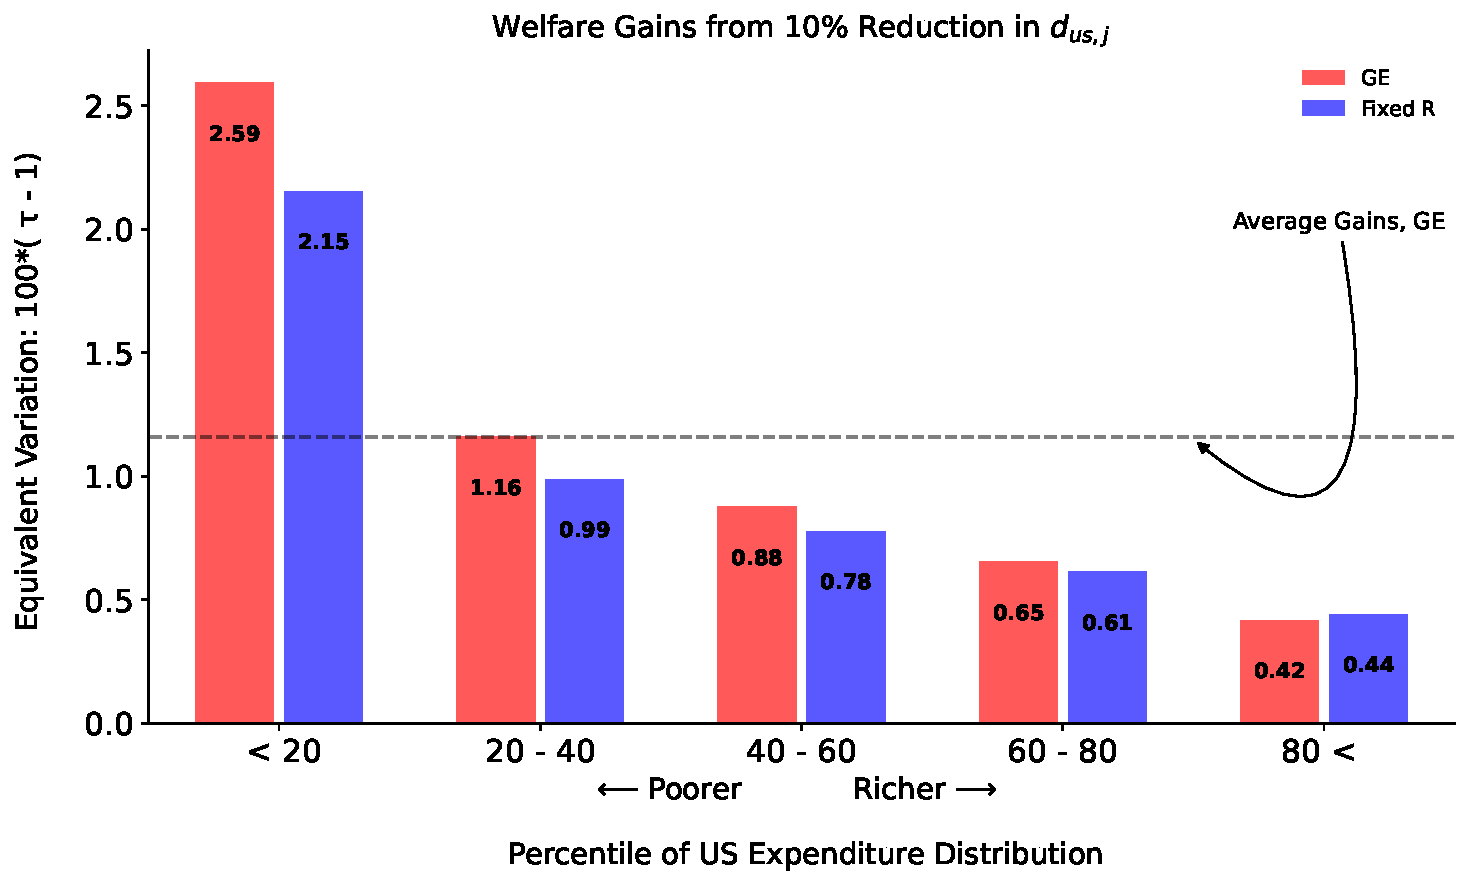
\includegraphics[scale = .55]{./figures/ge-welfare-household-fixR.pdf}}
\caption{Welfare Gains by Household: 10\% Reduction in $d_{us,j}$}\label{fig:welfare-households}
\end{figure}

The key force behind this result lies in the discussion around equation (\ref{eq:gains-substitution}) and how welfare changes. Two issues are at play: (i) how exposed a household to trade and (ii) how households value a price reduction. The model was calibrated so that exposure was roughly equal across the income distribution so the first force is not leading to heterogenous gains from trade. In contrast, the model was designed and calibrated to match the fact that poor households are very elastic with respect to price and, thus, strongly value a price reduction. So the second force is the component driving the pro-poor aspect of these gains from trade.\footnote{For example, I calibrated the model without quality shifters delivering a pattern of micro-level expenditure shares with the poor unexposed to trade similar Figure \ref{fig:micro-trade}. In this case, the equivalent variation gains are flat across the income distribution except for the vary poorest; in utils they are strongly increasing in income.}

\begin{table}[t]
\small
\begin{center}
\refstepcounter{table}
\setlength {\tabcolsep}{5.75mm}
\renewcommand{\arraystretch}{1.60}\label{tb-welfare}
\begin{tabular}[t]{l c c c}
\multicolumn{4}{c}{{\normalsize\textbf{Table \ref{tb-welfare}: 10\% Reduction in US Trade Costs: Interest Rates, Trade, Welfare}} }
\\ \hline \hline
& Baseline & GE & Fixed R \\
\cmidrule(lr){2-2} \cmidrule(lr){3-3} \cmidrule(lr){4-4}
US Imports / GDP & $7.2$ & $9.1$ & $9.2$  \\
$R - 1$ & $1.00$ & $0.8$ & $1.00$  \\
\hline
\multicolumn{2}{l}{Average Gains} & $1.2$ & $1.1$\\
\multicolumn{2}{l}{Ratio of Bottom 20 vs. Top 20 Welfare} & $6.1$ & $4.8$\\
\multicolumn{2}{l}{ACR Implied Gains } & $0.52$ & $0.53$ \\
\hline
\end{tabular}
\\[0.5ex]
\parbox{5.75in}{\footnotesize \textbf{Note:} Imports / GDP, Interest Rates, and Welfare are in percent. All values from the perspective of the US. Bottom 20 vs. Top 20 Welfare reports the ratio of household welfare for those in the bottom 20th percentile of the expenditure distribution vs. those at the top 20th.}
\end{center}
\end{table}

On average, the gains across households are much larger than representative agent benchmarks. The third row of Table \ref{tb-welfare} and the dashed line in Figure \ref{fig:welfare-households} show that the average gain is 1.2 percent. In contrast, a calculation of \citet{arkolakis2012new} off of the change in the US import share with an elasticity of four implies that the aggregate gains are only half a percent (bottom row of Table \ref{tb-welfare}).\footnote{I show in the appendix, the formula in \citet{arkolakis2012new} is equivalent variation measure as I compute and, hence, the large gains I'm finding are not because I add curvature to the utility function or having infinitely lived agents | these do not matter when computing equivalent variation.} This is half the size of the heterogenous agent model.

The reason why my model delivers larger gains is because of the large gains in the bottom part of the income distribution. Looking at Figure \ref{fig:welfare-households}, the gains from trade for the rich households look a lot like those that would come out of \citet{arkolakis2012new}-style calculation. However, for poor households, the gains are big as price changes matter a lot for these households.

Following the discussion around Proposition \ref{prp:gains-trade}, the other issue at play is how interest rates are changing and inducing valuation effects. The blue bars in Figure \ref{fig:welfare-households} report the gains when $R$ is fixed at its initial level and thus the asset market is not clearing, while all other prices are allowed to adjust. Thus, the comparison of the red vs. blue bars partials out the role that interest rates are playing.

There is only a modest effect of interest rates. Since intrust rates decline in the counterfactual, rich households gain slightly more ($0.44$ vs. $0.42$) when $R$ is held fixed. These households are those holding assets, are most effected by the decline in interest rates, but also loose less since they are rich and their marginal utility is low. For the poorest households the situation is flipped. They gain less ($2.15$ vs. $2.59$) when $R$ is held fixed. These are debtor households (or soon to be) and thus any decline in interest rates relaxes their budget constraint. And because these are high marginal utility households, the small change in interest rates is magnified for them.

Interest rates only change slightly there is financial globalization. While the US is the largest economy in the model, with 19 countries changes in US trade costs have small effects on global asset demand and supply.  In Section \ref{sec:asset-market}, I explore the alternative case with financial autarky where larger moves in domestic interest rates are observed.

\subsection{Heterogeneity by Trading Partner}


\begin{figure}[!t]
\centering{\includegraphics[scale = .5]{./figures/welfare-bilateral.pdf}}
\caption{Welfare Gains by Household: 10\% Reduction in $d_{us,j}$}\label{fig:welfare-households}
\end{figure}


\subsection{The Role of the Asset Market}\label{sec:asset-market}






%\section{Trade in the Efficient Allocation}
%
%This section computes what the pattern of trade \emph{should} look like were we living in a first-best world.
%
%\begin{figure}[!t]
%\centering{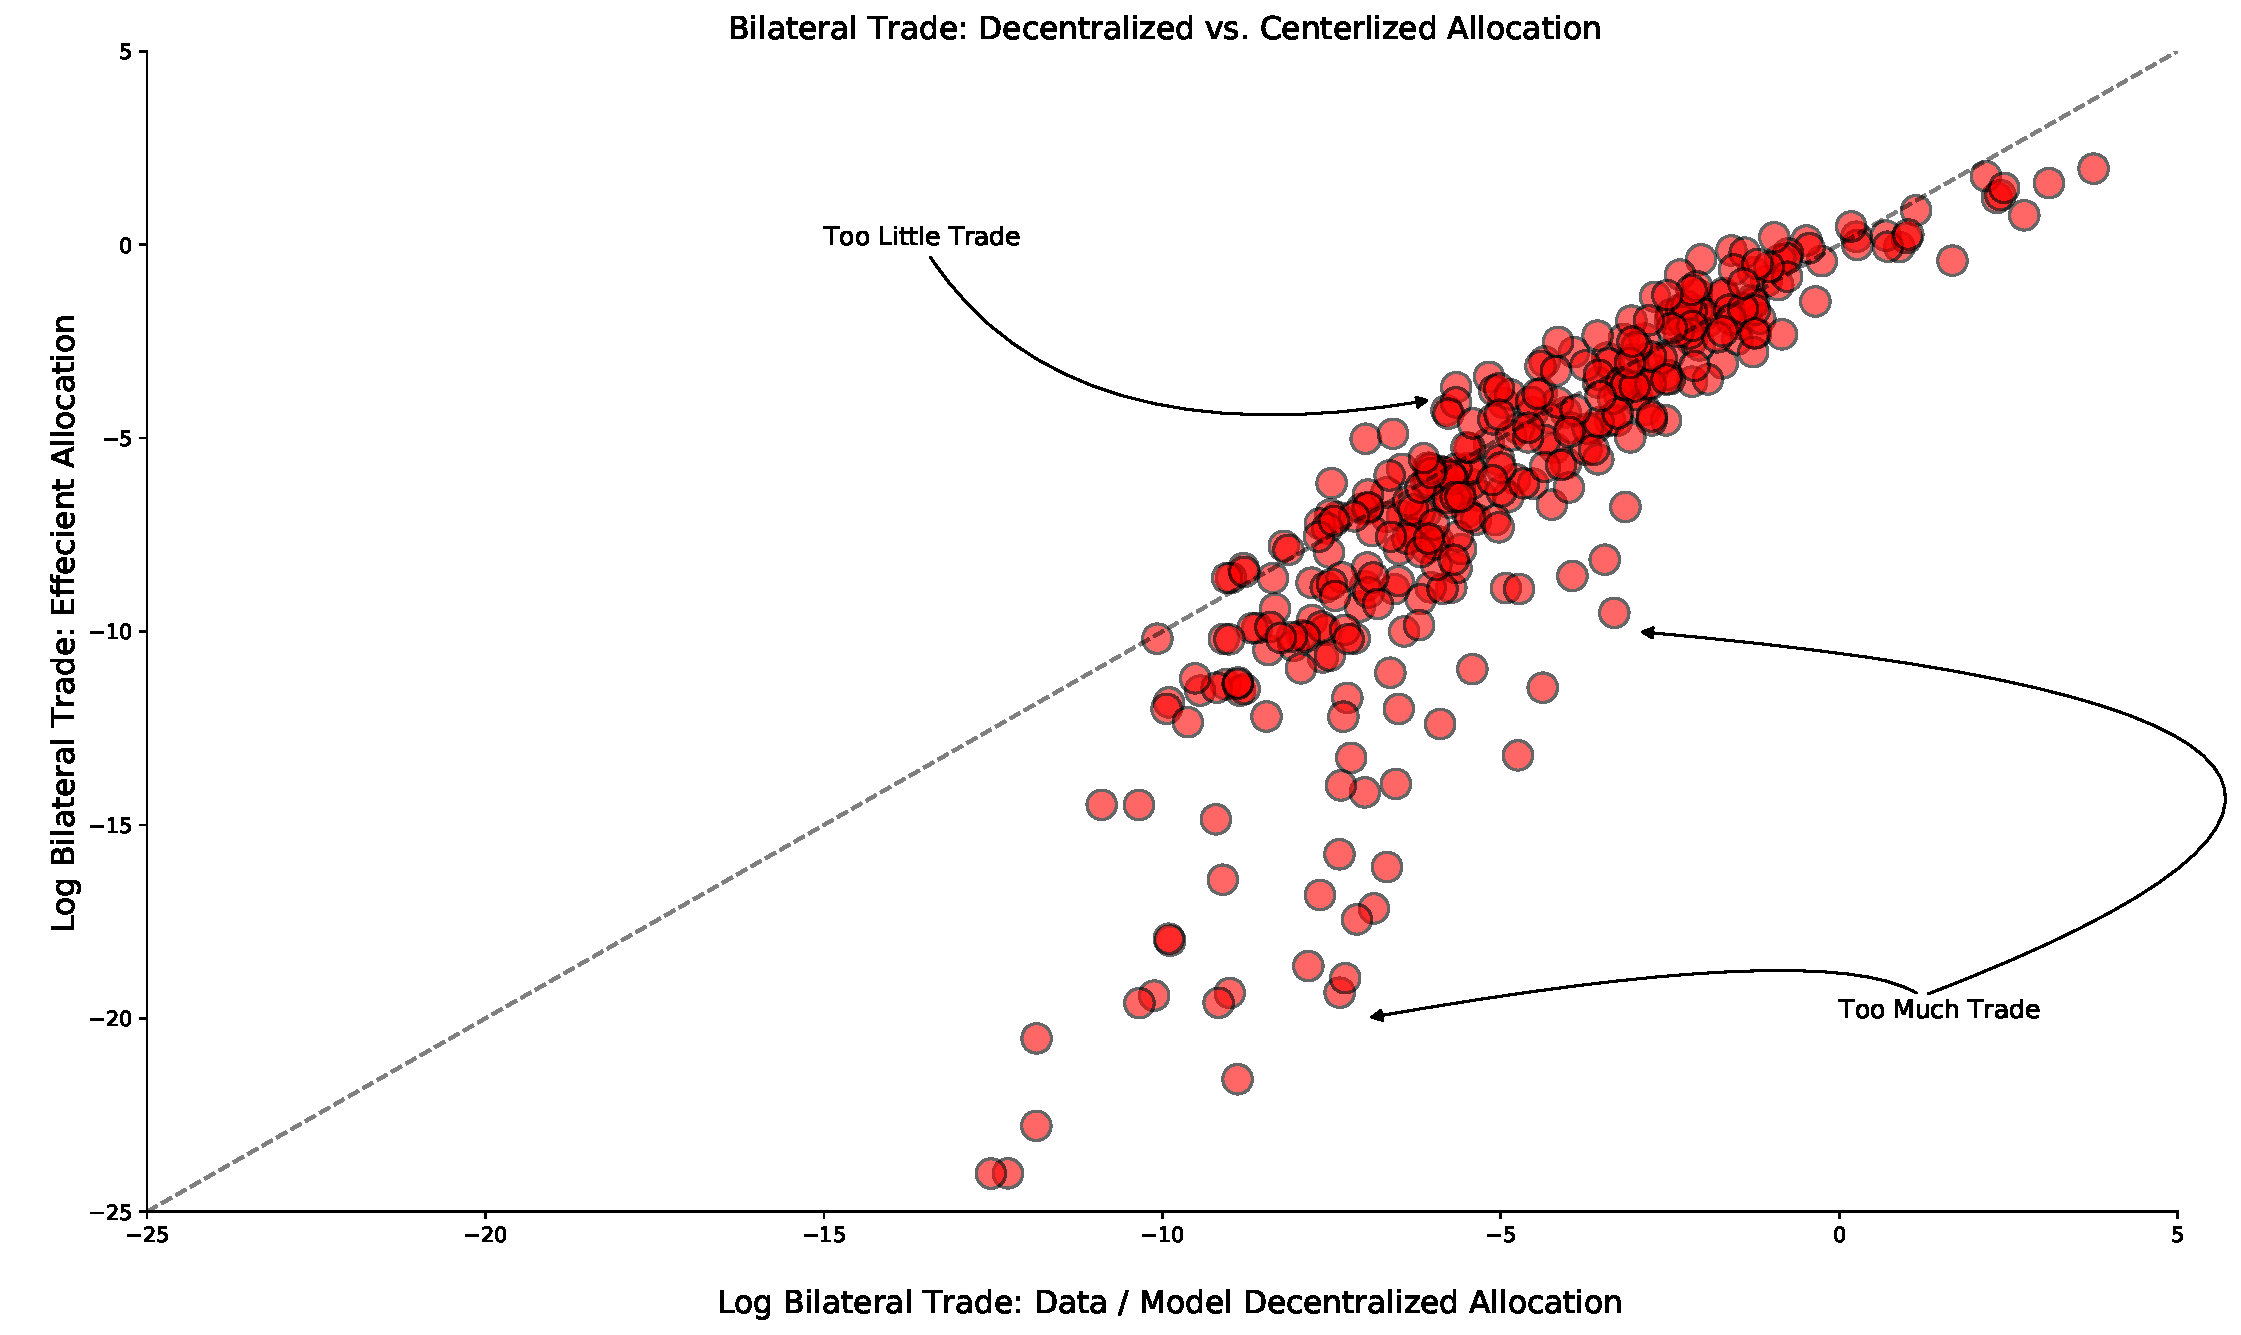
\includegraphics[scale = .45]{./figures/decentralized-trade-all.pdf}}
%\caption{}\label{fig:planner-trade}
%\end{figure}
%
%Before getting into the results, an important input into computing the allocation in Proposition \ref{prp:efficient-allocation} are the Pareto weights. I set the Pareto weight for a country to be proportional to it's level of TFP. My rationale behind this choice of weights is to eliminate the Planners incentives to shift consumption across countries vs. margins within the country. More specifically, this specification limits the planners desire to redistribute consumption from say, the US (a rich country) to Greece (a poor country in the data set) and focuses the exercise on within country redistribution.
%
%Given the Pareto weights, I take the parameters of the model and then compute consumption allocations and trade flows that solve planning problem described in Section \ref{sec:planner}. To be clear, there is no change in trade costs | all the planner is doing is redistributing and overcoming market incompleteness that is present in the decentralized allocation.
%
%\subsection{Efficient Trade}
%
%Figure \ref{fig:planner-trade} illustrates what the pattern of trade should look like from the planners perspective. The x-axis of Figure \ref{fig:planner-trade} plots log bilateral trade flows in the model (and data) in the decentralized equilibrium. So the same thing as in Figure \ref{fig:model-fit}. The y-axis reports the trade flows in the efficient allocation. The 45-degree line is drawn so if the red-dots lie on this line, this means that trade in the efficient allocation lines up with the decentralized allocation.
%
%Generally they do not line up on the 45-degree line. Two types of deviations stand out. First, small trade flows tends to be made smaller. From the planners perspective these are not efficient trading relationships. In contrast, large trading relationships are generally not large enough, this is the set of dots lying from about -5 to 0. So there is a meaningful sense that the Planner wants a reallocation of how households source goods.
%
%Figure \ref{fig:planner-vs-data} further illustrates this reallocation by focusing on how US imports change. The left panel reports import shares in the model (and data). Here you can see that the aggregate import share is about 7 percent with Canada, Japan, and some other European countries contributing to the bulk of US imports.
%
%In the efficient allocation the planner simultaneously wants the US to trade \emph{more}, but concentrate US imports on it's most productive (and large) partner which is Japan, a bit more from Germany, and less from Canada. And small trade flows with the potpourri of the remaining countries are made much smaller consistent with Figure \ref{fig:planner-trade}.
%
%The issue is this: uncompetitive source countries are ``luxuries'' from the planners perspective. In the decentralized equilibrium, the varieties from these countries are only purchased from rich households (and have the appearance of being luxuries as they are also high elasticity goods). Then, when the planner equalizes consumption within a country, the demand for these goods is eliminated.
%
%Why does trade expand in certain directions? There is an optimistic message here: the US is under-utilizing other productive countries via trade as a means to increase consumption for the masses. This is why trade expands with Japan which in the calibrated economy is very productive with a large labor force.
%
%\begin{figure}[!t]
%\begin{subfigure}{0.5\textwidth}
%    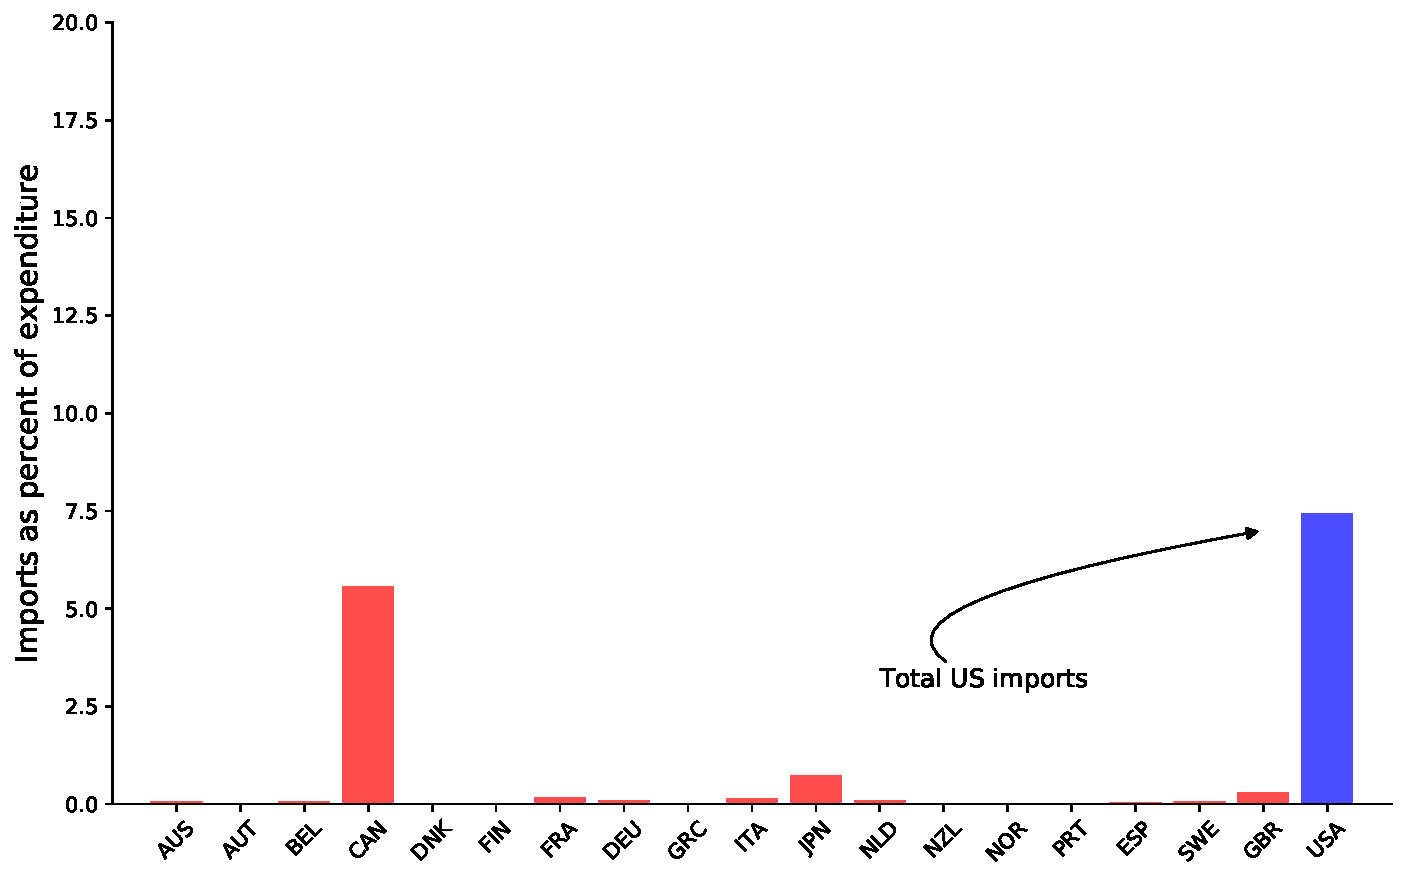
\includegraphics[scale = 0.36]{./figures/decentralized-trade-us.pdf}
%    \caption{{Trade in the Decentralized Allocation}}\label{fig:us-data-trade}
%\end{subfigure}
%\hspace{0.01cm}
%\begin{subfigure}{0.5\textwidth}
%    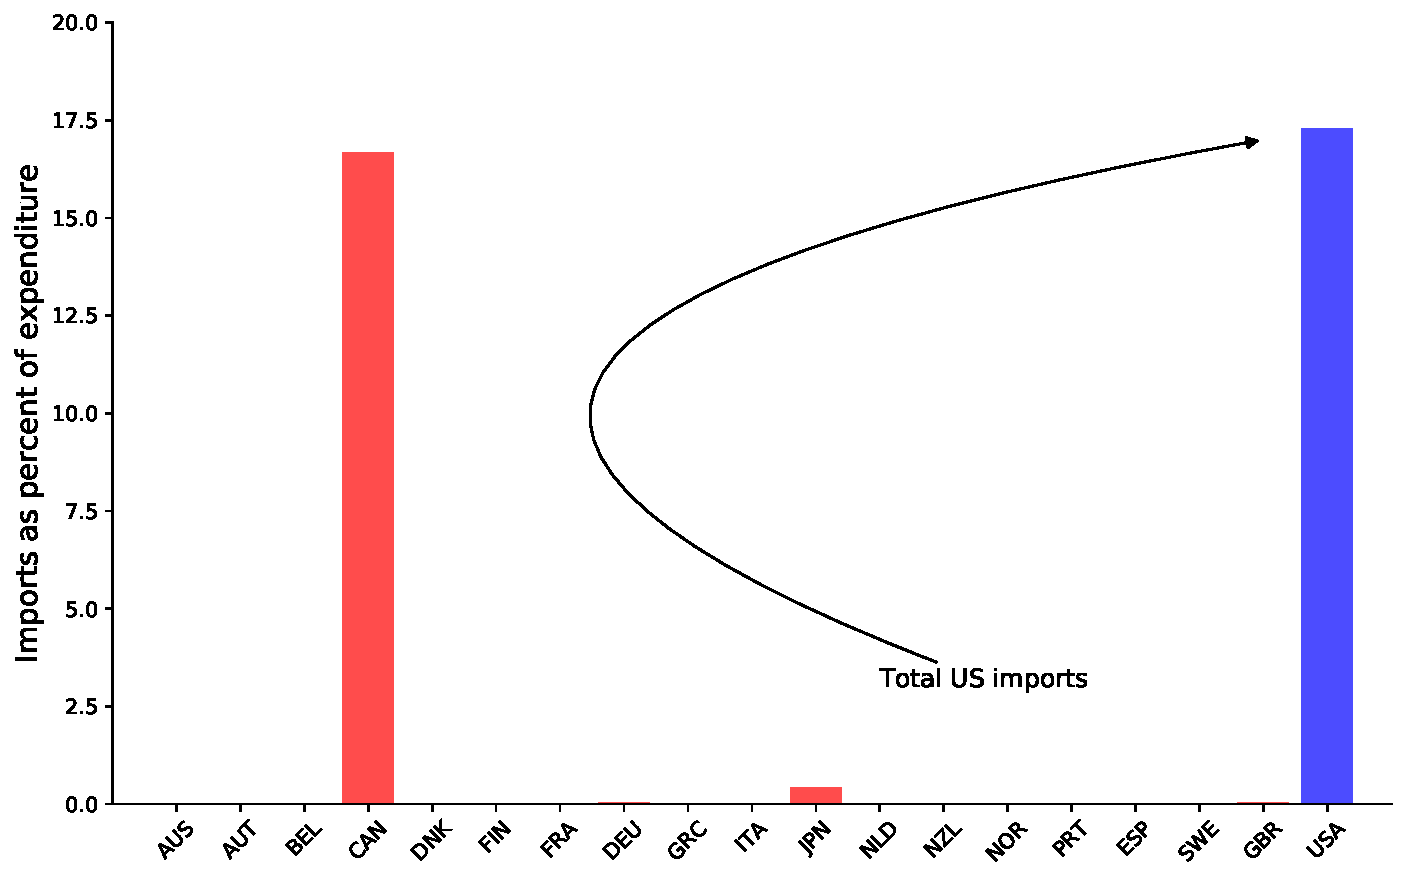
\includegraphics[scale = 0.36]{./figures/planner-trade-us.pdf}
%    \caption{{Trade in the Efficient Allocation}}\label{fig:us-planner-trade}
%\end{subfigure}
%\caption{US imports: Decentralized vs. Centralized Pattern of Trade}\label{fig:planner-vs-data}
%\end{figure}


\section{Conclusion}

What do you find interesting? Email me.



\appendix

\clearpage
\newpage

\begin{center}
\textbf{\Large Appendix}
\end{center}

\addcontentsline{toc}{section}{Appendices}

\section{The H-A Trade Elasticity}

My definition of the trade elasticity is the partial equilibrium response of imports from j relative
to domestic consumption due to a permanent change in trade costs. By partial equilibrium, I
mean that wages, interest rates, and the distribution of agents are fixed at their initial equilibrium values. This is consistent with the definition of the trade elasticity in say, \citet{arkolakis2012new} and \citet{simonovska2014elasticity}. By permanent, I mean that the change in trade costs is for the indefinite future and that households correctly understand this. Consistent with this discussion and the notation below, I compute the partial derivatives (not total) of objects with respect to trade costs.

Mathematically, the trade elasticity equals the difference between the elasticities for how trade between $i$ and $j$ change minus how home trade changes:
\begin{align}
\frac{\partial ( M_{ij} / M_{ii} )}{\partial d_{ij}} \times \frac{d_{ij}}{( M_{ij} / M_{ii} )} =& \frac{\partial M_{ij} / M_{ij}}{\partial d_{ij} / d_{ij}}  - \frac{\partial M_{ii} / M_{ii}}{\partial d_{ij} / d_{ij}}.
\label{apx-eq:def_trade_elasticity}
\end{align}
The change in imports between $i$ and $j$ with respect to a change in trade costs is:
\begin{align}
\frac{\partial  M_{ij}}{\partial d_{ij}} = \int_{a,z} \bigg \{\frac{\partial p_{ij}}{\partial d_{ij}} c_{i}(a,z,j) \pi_{ij}(a,z) +  \frac{\partial c_{i}(a,z,j)}{\partial d_{ij}} p_{ij} \pi_{ij}(a,z) +
 \frac{\partial \pi_{ij}(a,z)}{\partial d_{ij}} p_{ij}c_{i}(a,z,j) \bigg \} L_i \lambda_{i}(a,z) da \ dz.
\end{align}
Divide the stuff on the inside of the brackets by household level imports, $p_{ij}c_{i}(a,z,j)\pi_{ij}(a,z)$ and multiply on the outside giving,
\begin{align}
\frac{\partial  M_{ij}}{\partial d_{ij}} = \int_{a,z}  \bigg \{ \frac{\partial p_{ij}/p_{ij}}{\partial d_{ij}}  + \frac{\partial c_{i}(a,z,j)/ c_{i}(a,z,j)}{\partial d_{ij}} +
 \frac{\partial \pi_{ij}(a,z) / \pi_{ij}(a,z)}{\partial d_{ij}}  \bigg \} p_{ij}c_{i}(a,z,j)\pi_{ij}(a,z) L_i \lambda_{i}(a,z)da \ dz.
\end{align}
Define the following ``weight'' which is the share of goods that those with states $a,z$ account for in total expenditures from $j$ as
\begin{align}
\omega_{ij}(a,z) = \frac{p_{ij}c_{i}(a,z,j)\pi_{ij}(a,z) L_i \lambda_{i}(a,z)}{M_{ij}},
\end{align}
where the sum of $\omega_{ij}(a,z)$ over states $a,z$ equals one. This gives a nice expression for the import elasticity
\begin{align}
\frac{\partial  M_{ij} / M_{ij}}{\partial d_{ij} / d_{ij}} = 1 + \int_{a,z} \bigg \{ \underbrace{ \frac{\partial c_{i}(a,z,j)/ c_{i}(a,z,j)}{\partial d_{ij} / d_{ij}} }_{\theta_{ij}(a,z)^{I}}+
\underbrace{\frac{\partial \pi_{ij}(a,z) / \pi_{ij}(a,z)}{\partial d_{ij} / d_{ij}} }_{\theta_{ij}(a,z)^{E}} \bigg \} \omega_{ij}(a,z)da \ dz,
\end{align}
or more succinctly as
\begin{align}
\frac{\partial  M_{ij} / M_{ij}}{\partial d_{ij} / d_{ij}} = 1 + \int_{a,z} \bigg \{ \theta_{ij}(a,z)^{I} + \theta_{ij}(a,z)^{E} \bigg \}\omega_{ij}(a,z)da \ dz.
\end{align}
where the elasticity of aggregate imports into $i$ from $j$ is a weighted average of several effects. The value one out in front arises from the complete pass-through of changes in trade costs to changes in prices and this is a bug of perfect competition market structure. Then the first term within the brackets represent the intensive margin $\theta_{ij}(a,z)^{I}$, so how much do quantities change conditional on choosing to consume variety $j$. The next term $\theta_{ij}(a,z)^{E}$ represents the extensive margin, so how the choice probabilities change.

To complete the derivation, I'll derive the own-imports term which is similar with
\begin{align}
\frac{\partial  M_{ii}}{\partial d_{ij}} = \int_{a,z} \bigg \{ \underbrace{\frac{\partial p_{ii}}{\partial d_{ij}} c_{ii}(a,z) \pi_{ii}(a,z)}_{ \ = \ 0} +  \frac{\partial c_{ii}(a,z)}{\partial d_{ij}} p_{ii} \pi_{ii}(a,z) + \frac{\partial \pi_{ii}(a,z)}{\partial d_{ij}} p_{ii}c_{ii}(a,z) \bigg \} L_i \lambda_{i}(a,z)da \ dz,
\end{align}
where the first-term is zero because this is a partial equilibrium elasticity. Then after constructing the proper weights and converting everything to elasticity form we have
\begin{align}
\frac{\partial  M_{ii} / M_{ii}}{\partial d_{ij} / d_{ij}} = \int_{a,z} \bigg \{ \theta_{ii,j}(a,z)^{I} + \theta_{ii,j}(a,z)^{E} \bigg \}\omega_{ii}(a,z)da \ dz,
\end{align}
where the $ii, j$ notation is that $\theta_{ii,j}(a,z)^{I}$ reflects how the intensive margin adjusts, conditional on a $ii$ choice, given a change in $ij$ price. Similarly, $\theta_{ii,j}(a,z)^{E}$ represents how the $ii$ choice probability changes given the $ij$ change in price.

Proposition \ref{prp:GET} then follows:

\setcounter{prp}{2}
\begin{prp}[\textbf{The H-A Trade Elasticity}]The trade elasticity between country $i$ and country $j$ is:
{\footnotesize
\begin{align}
\theta_{ij} = 1 + \int_{z,a} \bigg \{ \theta_{ij}(a,z)^{I} + \theta_{ij}(a,z)^{E} \bigg \}\omega_{ij}(a,z)da \ dz - \int_{z,a} \bigg \{ \theta_{ii,j}(a,z)^{I} + \theta_{ii,j}(a,z)^{E} \bigg \}\omega_{ii}(a,z)da \ dz
\label{apx-eq:trade-elasticity}
\end{align}
}which is an expenditure-weighted average of micro-level elasticities. The micro-level elasticities are decomposed into an intensive margin and extensive margin
{\footnotesize
\begin{align}
\nonumber
\theta_{ij}(a,z)^{I} = \frac{\partial c_{i}(a,z,j)/ c_{i}(a,z,j)}{\partial d_{ij} / d_{ij}}, \ \ \ \ \ \ \theta_{ij}(a,z)^{E} = \frac{\partial \pi_{ij}(a,z) / \pi_{ij}(a,z)}{\partial d_{ij} / d_{ij}}, \ \ \ \
\end{align}
}
and the expenditure weights are defined as
{\footnotesize
\begin{align}
\nonumber
\omega_{ij}(a,z) = \frac{p_{ij}c_{i}(a,z,j)\pi_{ij}(a,z) \lambda_{i}(a,z) L_i}{M_{ij}}.
\end{align}
}
\end{prp}

\subsection{Connecting Household Behavior with Elasticities}

To derive the \textbf{intensive margin elasticity}, simply start from the households budget constraint and differentiate consumption of variety $j$ with respect to price $p_{ij}$ and one gets
\begin{align}
\underbrace{\frac{\partial c_{i}(a,z,j)/ c_{i}(a,z,j)}{\partial d_{ij} / d_{ij}}}_{\theta_{ij}(a,z)^{I}} &= \bigg [-\frac{\partial g_{i}(a,z,j)/ p_{ij}c_{i}(a,z,j)}{\partial p_{ij}/ p_{ij}} - 1 \bigg ]\frac{\partial p_{ij}/p_{ij}}{\partial d_{ij}/ d_{ij}} ,
\label{eq:apx-intensive-margin}
\end{align}
where recall that $g_{ij}(a,z)$ is the policy function mapping states into asset holdings next period $a'$. To derive the \textbf{extensive margin elasticity}, start from the definition of the choice probability and one finds
\begin{align}
\underbrace{ \frac{\partial \pi_{ij}(a,z) / \pi_{ij}(a,z)}{\partial d_{ij} / d_{ij}} }_{\theta_{ij}(a,z)^{E}} &= \frac{1}{\sigma_{\epsilon}}\frac{\partial v_{i}(a, z, j)}{\partial d_{ij}/d_{ij}} -  \frac{\partial \Phi_{i}(a,z) / \Phi_{i}(a,z)}{\partial d_{ij}/d_{ij}}.
\label{eq:apx-extensive-margin}
\end{align}
And then I use the following arguments to unpack how the value function $v_{i}(a, z, j)$ changes:
\begin{align}
\frac{\partial v_{i}(a,z,j)}{\partial d_{ij}/d_{ij}}  =& -u'(c_{i}(a,z,j))c_{i}(a,z,j) + \bigg [ -\frac{u'(c_{i}(a,z,j))}{p_{ij}}\frac{\partial g_{i}(a,z,j)}{\partial p_{ij}/ p_{ij}} \bigg ]  \\
\nonumber \\
&+ \beta \mathrm{E} \bigg \{\frac{\partial v}{\partial a'}\frac{\partial g_{i}(a,z,j)}{\partial p_{ij}/ p_{ij}}\frac{ \partial p_{ij}/ p_{ij}}{\partial d_{ij}/ d_{ij}} +  \frac{\partial v(g_{i}(a,z,j),z')}{\partial p_{ij}/ p_{ij}}\frac{ \partial p_{ij}/ p_{ij}}{\partial d_{ij}/ d_{ij}} \bigg \}
\end{align}
which can then be further expressed in terms of the Euler Equation (derived below in Equation (\ref{eq:apx-euler-equation}))
\begin{align}
\frac{\partial v_{i}(a,z,j)}{\partial d_{ij}/d_{ij}}  =& -u'(c_{i}(a,z,j))c_{i}(a,z,j) \label{eq:apx-first-term}\\
\nonumber \\
&+ \underbrace{\bigg \{ -\frac{u'(c_{i}(a,z,j))}{p_{ij}} + \beta \mathbb{E} \bigg [ -\sigma_{\epsilon} \frac{\partial \pi_{ii}(a',z') / \pi_{ii}(a',z')}{\partial a'} + u'(c_{i}(a',z',i))R \bigg ] \bigg \} }_{\mbox{Euler equation in (\ref{eq:apx-euler-equation})}} \frac{\partial g_{i}(a,z,j)}{\partial p_{ij}/ p_{ij}} \\
\nonumber \\
&+  \beta \mathbb{E}\frac{\partial v_{i}(a',z')}{\partial p_{ij}/ p_{ij}} \bigg \}
\end{align}
The term in the second line: the Euler equation multiplied by how assets change should be zero for small changes. I discuss this more in depth below around the welfare gains calculation, but the key issue is that either the Euler equation holds and thus this term is zero, or it does not hold, but then households can't adjust asset holdings and then the outside part is zero. And for small changes households on the margin of a binding constraint or not are on the margin and don't matter.

The final step is to connect the first term in (\ref{eq:apx-first-term}) with things like the relative risk aversion and the marginal propensity to consume. So specifically, thought experiment here is ignore all the future effects and ask if a household was a bit wealthier what would the effect be on the $u'(c_{ij}(a,z))c_{ij}(a,z)$ and hence how one component of the extensive margin elasticity changes:
\begin{align}
\frac{\partial (u'(c_{ij}(a,z))c_{ij}(a,z))}{\partial a} =& u''(c_{ij}(a,z))\frac{\partial c_{ij}}{\partial a}c_{ij}(a,z) + u'(c_{ij}(a,z))\frac{\partial c_{ij}}{\partial a} \\
\nonumber \\
&= \frac{\partial c_{ij}}{\partial a}\bigg[u''(c_{ij}(a,z))c_{ij}(a,z) + u'(c_{ij}(a,z)) \bigg] \\
\nonumber\\
&= u'(c_{ij}(a,z))\times \mathbf{MPC}_{ij}(a,z) \times \bigg[-\rho_{ij}(a,z) + 1\bigg]. \label{eq:apx-elasticity-mpc}
\end{align}
And just to emphasize how this works, it's a derivative of $u'(c_{ij}(a,z))c_{ij}(a,z)$. So as assets go up, with $\rho > 1$ this implies that $u'(c_{ij}(a,z))c_{ij}(a,z)$ goes down! And this is a force for things to be less elastic for rich guys. As assets go down, this implies that $u'(c_{ij}(a,z))c_{ij}(a,z)$ goes up, and this is a force for poor guys to be more elastic.

The final elasticity I want to derive is how home choices respond to changes in trade frictions. This is a term that shows up all the time (in the calculations above) and in the welfare expressions, so it's worth computing as well:
\begin{align}
\frac{\partial \pi_{ii}(a,z) / \pi_{ii}(a,z) }{\partial d_{ij} / d_{ij}} = \frac{1}{\sigma_{\epsilon}}\frac{\partial v_{i}(a,z,i)}{\partial d_{ij}/d_{ij}} - \frac{\partial \Phi_{i}(a,z) / \Phi_{i}(a,z)}{\partial d_{ij}/d_{ij}}.
\end{align}
Then the derivative of the term $\Phi$ takes on a unique property where
\begin{align}
\frac{\partial \Phi_{i}(a,z) / \Phi_{i}(a,z)}{\partial d_{ij}/d_{ij}} = \sum_{j} \pi_{ij}(a,z) \frac{1}{\sigma_{\epsilon}}\frac{\partial v_{i}(a,z,j)}{\partial d_{ij}/d_{ij}}
\end{align}
which takes on this flavor of exposure (which are the home choice probabilities) times how the household's valuations across the goods change (as represented by the value functions). Then expressing things all relative to how the home valuation changes we have
\begin{align}
\frac{\partial \pi_{ii}(a,z) / \pi_{ii}(a,z) }{\partial d_{ij} / d_{ij}} = \frac{1}{\sigma_{\epsilon}} \sum_{j} \pi_{ij}(a,z) \bigg[ \frac{\partial v_{i}(a,z,i)}{\partial d_{ij}/d_{ij}} - \frac{\partial v_{i}(a,z,j)}{\partial d_{ij}/d_{ij}} \bigg].
\label{eq:apx-change-home-choice}
\end{align}
So what this says is that the change in the home choice completely summarizes how things change (in a relative sense).

\section{The Welfare Gains from Trade}\label{apx-sec:gains-trade}

This section derives the gains from a permanent change in trade costs, across steady states. Like the discussion above, the idea here is that I'm thinking a situation where the change is small and there is an immediate jump to the new steady state. Unlike the trade elasticity, I'm going to take total derivatives encompassing general equilibrium changes in wages and interest rates.

The analysis proceeds in several steps.

First, I'll focus on country $i$ and study a change in trade costs $d_{ij}$. To simplify the algebra, I choose $w_i$ to be the numeraire and normalize $A_i = 1$. This implies is that $p_{ii} = \frac{w_i}{A_i}$ equals one and it's derivative with respect to things is zero.

Second, To compute how social welfare changes, I focus on a utilitarian social welfare function (Pareto weights across households, within a country, are the same):
\begin{align}
W_{i} = \int_{a}\int_{z}  v_{i}(a,z)\lambda_{i}(a,z)
\label{eq:apx-social-welfare}
\end{align}
Then the total change in total welfare is
\begin{align}
\frac{\mathrm{d} W_{i}}{\mathrm{d} d_{ij} / d_{ij}} = \int_{a}\int_{z}  \bigg \{ \frac{\mathrm{d} v_i(a, z)}{\mathrm{d} d_{ij} / d_{ij}}  + v_{i}(a,z) \frac{\mathrm{d} \lambda_{i}(a,z)/ \lambda_{i}(a,z)}{\mathrm{d} d_{ij} / d_{ij}}  \bigg \} \lambda_{i}(a,z).
\label{eq:apx-social-welfare-change}
\end{align}
The first component reflects changes in household-level welfare. The second component is about reallocation, i.e., if|at the old $v$'s|does the distribution change so that social welfare gets better or worse. The change in social welfare is then the weighted average of these two forces with the weights being those at the initial distribution.

How does household-level welfare change? I'm going to walk through this in several steps.

First, I show how I can express everything relative to the home country $i$. Recall that the value function (with the expectation taken over the different preference shocks) is
\begin{align}
v_i(a, z) =  \sigma_{\epsilon} \log \left\{ \sum_{j'} \exp \left( \frac{  v_{i}(a, z, j')}{\sigma_{\epsilon}} \right) \right\},
\label{eq:apx-epsilon-vfun}
\end{align}
and then I'm going to make the observation that I can substitute out the sum part (\ref{eq:apx-epsilon-vfun}) with the exp of the home value function relative to the micro-level ``home choice'' so
\begin{align}
\pi_{ii}(a, z) = \exp \left( \frac{ v_{i}(a, z, i) }{\sigma_{\epsilon}} \right) \Bigg / \sum_{j'} \exp \left( \frac{ v_{i}(a, z, j') }{\sigma_{\epsilon}} \right), \\
\nonumber \\
\pi_{ii}(a, z) \times \sum_{j'} \exp \left( \frac{ v_{i}(a, z, j') }{\sigma_{\epsilon}} \right) = \exp \left( \frac{ v_{i}(a, z, i) }{\sigma_{\epsilon}} \right), \\
\nonumber \\
\sum_{j'} \exp \left( \frac{ v_{i}(a, z, j') }{\sigma_{\epsilon}} \right) = \exp \left( \frac{ v_{i}(a, z, i) }{\sigma_{\epsilon}} \right) \Bigg / \pi_{ii}(a, z).
\label{eq:apx-homeshare-vfun}
\end{align}
Then substituting (\ref{eq:apx-homeshare-vfun}) into the value function in (\ref{eq:apx-epsilon-vfun}) gives:
\begin{align}
v_i(a, z) =  \sigma_{\epsilon} \log \left\{ \frac{ \exp \left( \frac{  v_{i}(a, z, i)}{\sigma_{\epsilon}}\right )}{\pi_{ii}(a,z)}  \right\}
\label{eq:apx-homeshare-vfun2}
\end{align}
and recall that the home choice value function is
\begin{align}
v_{i}(a, z, i) = u(c_{i}(a,z,i)) + \beta \mathbb{E} v_{i}(g_{i}(a,z,i),z)
\end{align}
where the expectation operator is over the $z$s and the $v_{i}$ is the same value function as in (\ref{eq:apx-epsilon-vfun}) so the taste shocks are integrated out. Taking logs and exp's of (\ref{eq:apx-homeshare-vfun2}) allows for the $v_i$ value function to be represented as
\begin{align}
v_i(a, z) = -\sigma_{\epsilon} \log \pi_{ii}(a,z) + u(c_{i}(a,z,i)) + \beta \mathbb{E} v_{i}(g_{i}(a,z,i),z).
\label{eq:apx-home-valuefun}
\end{align}
Now everything is written with respect to the home choice. What is going on is that the home choice $\pi_{ii}$ summarizes the expected value of those shocks and their benefits. No need to explicitly carry around the $v_{ij}$s. This is essentially the dynamic analog to Equation (15), Footnote 42 of \citet{eaton2002technology} and \citet{arkolakis2012new}.

Now the strategy is to totally differentiate (\ref{eq:apx-home-valuefun}) with respect to trade costs and use the recursive structure to iterate forward and construct the change across time.  One more detail, to facilitate interpretation, it will be useful to compute the Euler equation associated with asset holdings when the borrowing constraint does not bind. This euler equation is:
\begin{align}
-u'(c_{i}(a,z,i)) = \beta \mathbb{E} \bigg \{ -\sigma_{\epsilon} \frac{\partial \pi_{ii}(a',z') / \pi_{ii}(a',z')}{\partial a'} + u'(c_{i}(a',z',i))R \bigg \},
\label{eq:apx-euler-equation}
\end{align}
which says that the agent should be indifferent between the marginal utility of consumption forgone to hold some more assets and two components (i) the benefit from how a change in assets changes in their variety choice and (ii) the direct benefit of the returns on the assets evaluated at the marginal utility of consumption.

%\hrulefill
%
%Redo. Digression on chain rule. I'm going to
%\begin{align}
%v(a',z') = v(g(a,z,d), z')
%\end{align}
%where I substitute in the policy function for $a'$. Then first term inside indicates that $v$ depends upon the choice of $a'$ and this works through the policy function. And the dependence of $v$ on $d$ (and not through assets) is implicit. Then the total derivative of this is
%\begin{align}
%\frac{\mathrm{d} v(g(a,z,d), z')}{\mathrm{d} d} =& \frac{\partial v}{\partial a'}\frac{\mathrm{d}g}{\mathrm{d}d} +  \frac{\partial v(\overline{g(a,z,d)},z')}{\partial d}
%\end{align}
%So the first term is the partial change of $v$ with respect to $a'$ times how the policy function totally changes with respect to $d$. The second term is the partial change of $v$ with respect to $d$, \textbf{holding fixed assets} at their chosen level. That's why I'm emphasizing the bar on top. Now what is confusing to me is that this has partial, not total derivatives. But this term is mathematically the same as
%\begin{align}
%\frac{\partial v(\overline{g(a,z,d)},z')}{\partial d} = \frac{\mathrm{d} v(a', z')}{\mathrm{d} d }
%\end{align}
%where the RHS is the total derivative of $v$ treating $a'$ as a parameter. In other words, the LHS says, how does $v$ change (everything else) holding fixed assets. The RHS says how does everything else change holding fixed assets. There the same. And the RHS is the value function evaluated at the new states $a'$, $z'$.
%
%\hrulefill

Totally differentiating the value function gives
\begin{align}
\frac{\mathrm{d} v_i(a, z)}{\mathrm{d} d_{ij} / d_{ij}} =& \nonumber  \\
\nonumber \\
 -\sigma_{\epsilon} & \frac{\mathrm{d} \pi_{ii}(a,z) / \pi_{ii}(a,z)}{\mathrm{d}d_{ij} / d_{ij}}  + u'(c_{i}(a,z,i))\frac{\mathrm{d} R}{\mathrm{d} d_{ij} / d_{ij}}a - u'(c_{i}(a,z,i))\frac{\mathrm{d} g_{ii}(a,z)}{\mathrm{d} d_{ij} / d_{ij}}
+ \beta E \frac{\mathrm{d} v_i(g_{i}(a,z,i), z')}{\mathrm{d} d_{ij} / d_{ij}}
\end{align}
Then the derivative of the continuation value function is:
\begin{align}
& \frac{\mathrm{d} v_i(g(a,z,i), z')}{\mathrm{d} d_{ij} / d_{ij}} = \underbrace{\bigg [-\sigma_{\epsilon} \frac{\partial \pi_{ii}(a',z') / \pi_{ii}(a',z')}{\partial a'} + u'(c_{i}(a',z',i))R \bigg ]}_{\frac{\partial v_i(g_{i}(a,z,i), z')}{\partial a}}\frac{\mathrm{d} g_{ii}(a,z)}{\mathrm{d} d_{ij} / d_{ij}} \ \ + \\
\nonumber \\
& -\sigma_{\epsilon} \frac{\mathrm{d} \pi_{ii}(a',z') / \pi_{ii}(a',z')}{\mathrm{d}d_{ij} / d_{ij}}   + u'(c_{i}(a',z',i))\frac{\mathrm{d} R}{\mathrm{d} d_{ij} / d_{ij}}a' - u'(c_{i}(a',z',i))\frac{\mathrm{d} g_{i}(a',z',i)}{\mathrm{d} d_{ij} / d_{ij}}
+ \beta E \frac{\mathrm{d} v_i(g_{i}(a',z',i), z'')}{\mathrm{d} d_{ij} / d_{ij}}
\end{align}
And now collect terms so
\begin{align}
\frac{\mathrm{d} v_i(a, z)}{\mathrm{d} d_{ij} / d_{ij}} =& -\sigma_{\epsilon} \frac{\mathrm{d} \pi_{ii}(a,z) / \pi_{ii}(a,z)}{\mathrm{d}d_{ij} / d_{ij}} \\
\nonumber \\
& + \underbrace{u'(c_{i}(a,z,i))\frac{\mathrm{d} R}{\mathrm{d} d_{ij} / d_{ij}}a}_{\gamma_{ii}(a,z)}  \\
\nonumber \\
& + \underbrace{\bigg \{- u'(c_{ii}(a,z)) + \beta \mathbb{E}_z \big [-\sigma_{\epsilon} \frac{\partial \pi_{ii}(a',z') / \pi_{ii}(a',z')}{\partial a'} + u'(c_{i}(a',z',i))R \big ] \bigg \}\frac{\mathrm{d} g_{i}(a,z,i)}{\mathrm{d} d_{ij} / d_{ij}}}_{\delta_{ii}(a,z)} \\
\nonumber \\
& + \beta \mathbb{E}_{z} \bigg \{ -\sigma_{\epsilon} \frac{\mathrm{d} \pi_{ii}(a',z') / \pi_{ii}(a',z')}{\mathrm{d}d_{ij} / d_{ij}} +  u'(c_{i}(a',z',i))\frac{\mathrm{d} R}{\mathrm{d} d_{ij} / d_{ij}}a' \ \  \ldots
\label{eq:apx-welfare-vterms}
\end{align}
Let me walk through the interpretation of each term:
\begin{itemize}
\item $-\sigma_{\epsilon} \frac{\mathrm{d} \pi_{ii}(a,z) / \pi_{ii}(a,z)}{\mathrm{d}d_{ij} / d_{ij}}$ is a gains from trade term. I expand more on this term below.

\item $u'(c_{i}(a,z,i))\frac{\partial R}{\partial d_{ij} / d_{ij}}a$ or what I'm labeling as $\gamma_{ii}(a,z)$ is what I would call how changes in goods trade facilitates leads to changes in asset trade.

\item The third term which I'm labeling as $\delta_{ii}(a,z)$  is the Euler equation for assets. Honestly, it's pretty cool the way this shows up here. But it should also zero out through some basic arguments. Let me expand on this.

    The idea is that if the household is unconstrained, then this term is zero as there is no gain through changes in asset behavior. Asset holdings are already chosen optimally so that margins are equated, thus, on the margin any benefit of lower trade costs on changes in asset behavior is zero. Essentially an application of the Envelope Theorem.

    Now in this economy, this term may not be zero because of borrowing constrained households, thus this term is positive. However, notice how the outside brackets is multiplied by the change in the asset policy function. Again, this is super cool. What this picks up is that if the household is constrained, then assets can't change so the outside term is zero and, thus, overall the second term is zero.

    Final point, then the only people that benefit and contribute to social welfare through these effects are those on the margin between constrained and not-constrained. But if they are on the margin between being constrained and not-constrained, then they are on their euler equation. More formally, these agents are those where, from the Generalized Euler equation in (\ref{eq:apx-euler_equation}), both terms under the max operator are equated, so
    \begin{align}
    \beta R_{i} \mathrm{E}_{z'} \left[ \sum_{j'} \pi_{ij}(a', z') \frac{u'(c_{ij}(a', z'))}{p_{ij}} \right]  = u' \left( \frac{R_i a + w_i - \phi_{i}}{p_{ij}} \right)
    \end{align}

\item The final term is about this continuing on into the infinite future.
\end{itemize}
Iterating on (\ref{eq:apx-welfare-vterms}) into the future, the gains from trade for a household with states $a,z$ today are
\begin{align}
\frac{\partial v_i(a, z)}{\partial d_{ij} / d_{ij}} = \mathbb{E} \sum_{t = 0}^{\infty} \beta^{t} \bigg \{ -\sigma_{\epsilon} \frac{\mathrm{d} \pi_{ii}(a_{t},z_{t}) / \pi_{ii}(a_{t},z_{t})}{\mathrm{d}d_{ij} / d_{ij}} + \gamma_{ii}(a_{t},z_{t}) + \delta_{ii}(a_{t},z_{t}) \bigg \}
\label{eq:apx-welfare-v}
\end{align}
Where the first component is the expected discounted gains from substitution, gains from asset trade and the relaxation of borrowing constraints. Combining (\ref{eq:apx-welfare-v}) and (\ref{eq:apx-social-welfare-change}) yields the following proposition for the gains from trade

\begin{prp}[\textbf{The Welfare Gains from Trade}] \label{apx-prp:gains-trade} The welfare gains from trade are given by
{\footnotesize
\begin{align}
\frac{\mathrm{d} W_{i}}{\mathrm{d} d_{ij} / d_{ij}} = \int_{a}\int_{z}  \bigg \{ \frac{\mathrm{d} v_i(a, z)}{\mathrm{d} d_{ij} / d_{ij}}  + v_{i}(a,z) \frac{\mathrm{d} \lambda_{i}(a,z)/ \lambda_{i}(a,z)}{\mathrm{d} d_{ij} / d_{ij}}  \bigg \} \lambda_{i}(a,z).
\nonumber
\end{align}
}which reflects the change in household level gains and how the distribution of households changes. Household level gains are given by
{\footnotesize
\begin{align}
\nonumber
\frac{\partial v_i(a, z)}{\partial d_{ij} / d_{ij}} = \mathbb{E} \sum_{t = 0}^{\infty} \beta^{t} \bigg \{ -\sigma_{\epsilon} \frac{\mathrm{d} \pi_{ii}(a_{t},z_{t}) / \pi_{ii}(a_{t},z_{t})}{\mathrm{d}d_{ij} / d_{ij}} + \gamma_{ii}(a_{t},z_{t}) + \delta_{ii}(a_{t},z_{t}) \bigg \}
\end{align}
}where each term represents:
\begin{itemize}
\item Gains from substitution: $-\sigma_{\epsilon} \frac{\mathrm{d} \pi_{ii}(a,z) / \pi_{ii}(a,z)}{\mathrm{d}d_{ij} / d_{ij}}$.

\item Gains from asset trade: $\gamma_{ij}(a,z) = u'(c_{ii}(a,z))\frac{\mathrm{d} R}{\mathrm{d} d_{ij} / d_{ij}}a$

\item Gains from relaxing borrowing constraints:
\begin{align}
\nonumber
\delta_{ii}(a,z) = \bigg \{- u'(c_{ii}(a,z)) + \beta \mathbb{E} \big [-\sigma_{\epsilon} \frac{\partial \pi_{ii}(a',z') / \pi_{ii}(a',z')}{\partial a'} + u'(c_{ii}(a',z'))R \big ] \bigg \}\frac{\mathrm{d} g_{ii}(a,z)}{\mathrm{d} d_{ij} / d_{ij}} = 0
\end{align}
which equals zero for small changes.
\end{itemize}
\end{prp}
The final step is to unpack the gains from substitution term. Now from the elasticity discussion we can simply convert (\ref{eq:apx-change-home-choice}) into a total derivative
\begin{align}
\frac{\mathrm{d} \pi_{ii}(a,z) / \pi_{ii}(a,z) }{\mathrm{d} d_{ij} / d_{ij}} = \frac{1}{\sigma_{\epsilon}} \sum_{j'} \pi_{ij'}(a,z) \bigg[ \frac{\mathrm{d} v_{i}(a,z,i)}{\partial d_{ij}/d_{ij}} - \frac{\mathrm{d} v_{i}(a,z,j')}{\mathrm{d} d_{ij}/d_{ij}} \bigg].
\end{align}
so change in the home choice summarizes two forces: (i) how exposed a household is to the change through the choice probabilities and then (ii) how value functions change.

Now the value function component is where elasticities enter. To see this, define $\bar{\theta}(a,z) ^E_{ij',j}$ as the extensive margin, cross-price elasticity, and in total derivative form. Following the derivation of (\ref{eq:apx-extensive-margin}) this is
\begin{align}
\theta_{ij',j}(a,z)^{E} = \frac{1}{\sigma_{\epsilon}}\frac{\mathrm{d} v_{i}(a, z, j')}{\partial d_{ij}/d_{ij}} -  \frac{\mathrm{d} \Phi_{i}(a,z) / \Phi_{i}(a,z)}{\mathrm{d} d_{ij}/d_{ij}},
\end{align}
which then noticing that the $\mathrm{d} \Phi$ term is independent of option $j'$ and so they difference out, we can express in terms of cross-price elasticities
\begin{align}
-\sigma_{\epsilon} \frac{\mathrm{d} \pi_{ii}(a,z) / \pi_{ii}(a,z) }{\mathrm{d} d_{ij} / d_{ij}} = \sigma_{\epsilon} \sum_{j'} \pi_{ij'}(a,z) \bigg[ \bar{\theta}(a,z) ^E_{ii,j} - \bar{\theta}(a,z) ^E_{ij',j}\bigg],
\end{align}
Now there is one more way to express things that is also informative. \textbf{Assume that all cross-terms are near zero.} Then we have
\begin{align}
-\sigma_{\epsilon} \frac{\mathrm{d} \pi_{ii}(a,z) / \pi_{ii}(a,z) }{\mathrm{d} d_{ij} / d_{ij}} \approx
- \sigma_{\epsilon} \times \pi_{ij}(a,z) \times \bar{\theta}(a,z) ^E_{ij}
\end{align}
This expression is interesting because now it is analogous to the gains from trade formula in the efficient allocation. The pure gains from trade component comes from (i) how the taste shock are valued (and this is standard) (ii) a households exposure and (iii) the household's elasticity. And this last part, more or less reflects how sensitive the value function is with respect to price.

\newpage

\section{The Gains From Trade in the Efficient Allocation}\label{sec:apx-planner}

This section of the appendix presents abbreviated results from my related paper in \citet{waughoptimal}. Below I discus the planning problem, I state the solution to it, then discuss how I arrive at the gains from trade calculations in Proposition \ref{prp:gains-efficient-allocation}.

I focus on a utilitarian social welfare function with Pareto weights that vary across countries:
\begin{align}
W = \sum_{t=0}^{\infty} \sum_{i}  \int\limits_{z} \beta^{t}  v_{i}(z,t) L_{i}\lambda_{i}(z,t),
\label{eq:apx-social-welfare}
\end{align}
and here $v_i$ a households utility in country $i$. Now, I'm going to place the social welfare function in sequence space and then unpack the benefits from the preference shock in the following way:
\begin{align}
W = \sum_{t=0}^{\infty}  \sum_{i}  \sum_{j}  \int\limits_{z}  \beta^{t} \   \bigg \{  u(c_{i}(z, j, t) ) + \mathrm{E}[ \ \epsilon \ | \ \pi_{ij}(z,t) ] \bigg \}\pi_{ij}(z,t) L_{i} \lambda_{i}(z, t)
\label{eq:apx-social-welfare-2}
\end{align}
so the inner term is period utility given the associated consumption allocation $c_{ij}$ and then the expected value of the preference shock conditional on the choice probability $\pi_{ij}(z,t)$. This inner term is then weighted by the number of households that receive that utility, i.e. the choice probability times the mass of households with shock $z$ at date $t$. The sum across $j$ adds up all households in country $i$. Then the sum across $i$ reflects that this is global welfare.

One more point about the inner term in (\ref{eq:apx-social-welfare-2}), my claim is that with the Type 1 extreme value shocks:
\begin{align}
\mathrm{E}[ \ \epsilon \ | \ \pi_{ij}(z,t) ] = -\sigma_{\epsilon} \log \pi_{ij}(z,t)
\end{align}
where this is like the ``selection correction'' where if $\pi$ becomes smaller, the expected value of the taste shock becomes larger. So only those with the largest relative shocks are chosen and higher utility for those, conditional on being selected, is felt.

Given this formulation, the planner does the following: he chooses consumption and choice probabilities for all country pair combinations, state by state, for the infinite future. The Lagrangian associated with the Planning Problem is:
\begin{align}
\mathcal{L}  = & \sum_{t=0}^{\infty}   \sum_{i} \sum_{j} \int\limits_{z}  \beta^{t} \  \bigg \{  u(c_{i}(z, j, t) ) + \mathrm{E}[ \ \epsilon \ | \ \pi_{ij}(z,t) ] \bigg \}\pi_{ij}(z,t) L_{i} \lambda_{i}(z, t), \\
\nonumber \\
&+ \sum_{t=0}^{\infty} \sum_{i} \beta^{t} \chi_{i}(t) \bigg \{ Y_{it} \  - \ \sum_{j} \int\limits_{z}  d_{ji} c_{j}(z, i, t) \pi_{ji}(z,t) L_{j}\lambda_{j}(z, t) \bigg \} \nonumber \\
\nonumber \\
&+ \sum_{t=0}^{\infty} \sum_{i} \int\limits_{z}  \beta^{t} \chi_{2i}(z,t) \bigg \{1 - \sum_{j}\pi_{ij}(z,t) \bigg \} L_{i} \lambda_{i}(z, t), \nonumber
\label{apx-eq:planner_problem}
\end{align}
where the first term is the objective function; the second line is the resource constraint saying that output from country $i$ must equal the consumption of commodity $i$ globally including the transport costs. Then the third line ensures that choice probabilities are probabilities and sum to one. The final thing I'm doing is that I'm scaling the multipliers by $\beta^t$ so that the algebra is easier.

The statement below characterizes the allocation that solves (\ref{apx-eq:planner_problem}):
\begin{prp}[\textbf{The Efficient Allocation}]\label{apx-prp:efficient-allocation} The allocation that satisfies the Centralized Planning Problem in (\ref{apx-eq:planner_problem}) is:
\begin{enumerate}
\item A consumption allocation satisfying:
\begin{align}
 u'(c_{ij}(z,t) ) = \chi_{j}(t) d_{ij}
\end{align}
where $\chi_{j}(t)$ is the shadow price of variety $j$.
\item The choice probabilities are
\begin{align}
\pi_{ij}(t) =\exp \left( \frac{u(c_{ij}(t)) - u'(c_{ij}(t))c_{ij}(t)}{\sigma_{\epsilon}}\right) \bigg / \sum_{j'}\exp \left( \frac{u(c_{ij'}(t)) - u'(c_{ij'}(t))c_{ij'}(t)}{\sigma_{\epsilon}} \right)
\label{apx-eq:planner-choice-prob}
\end{align}
\end{enumerate}
\end{prp}

\textbf{The Gains from Trade.} Given this allocation, I want to compute the social gain to a change in trade costs. First, I express social welfare depending directly upon the trade costs $d$, and then indirectly as the allocations of $c$ and $\pi$s depend upon $d$ as well.
\begin{align}
W(d, c_{i}(j; d), \pi_{ij}(d))
\end{align}
And then totally differentiate social welfare, so
\begin{align}
\frac{\mathrm{d} W}{\mathrm{d}d} = \frac{\partial W}{\partial d} + \frac{\partial W}{\partial c_{i}(j;d)}\frac{\partial c_{i}(j;d)}{\partial d} + \frac{\partial W}{\partial \pi_{ij}(d)}\frac{\partial \pi_{ij}(d)}{\partial d}
\end{align}
and then I invoke the Envelope Theorem. That is I evaluate this derivative at the optimal allocation. But the optimal allocation is optimal, so on the margin any gain from changing consumption or choice probabilities is zero and these indirect effects (at the optimal allocation) are zero. Computing the direct effect gives
\begin{align}
\partial W = - & \sum_{t=0}^{\infty} \beta^{t} \ \chi_{j}(t) c_{i}(j,t) \pi_{ij}(t) L_{i} \partial d_{ij}, \\
\nonumber \\
=& - \sum_{t=0}^{\infty} \beta^{t} \  \ u'(c_{i}(j,t)) c_{i}(j,t) \pi_{ij}(t) L_{i} \partial d_{ij} / d_{ij},
\end{align}
where the first line simply is how the resource constraint in (\ref{apx-eq:planner_problem}) changes with respect to trade costs. Then the second line inserts the relationship between the multiplier and the marginal utility of consumption.  This says that the change in social welfare equals how much the resource constraint is relaxed by the change in trade costs. The $c_{ij}(t) \pi_{ij}(t) L_{i}$ term is how much stuff people in $i$ get from $j$ and $\partial d_{ij} / d_{ij}$ perturbs it by the percent change in trade costs, then $u'(c_{ij}(t))$ converts it into utils. Imposing stationarity delivers
\begin{align}
\frac{\mathrm{d} W}{\mathrm{d}d_{ij} / d_{ij}} = \frac{\partial W}{\partial d_{ij} / d_{ij}} = -\frac{ u'(c_{i}(j)) c_{i}(j) \pi_{ij} L_{i}}{1- \beta} \label{apx-eq:gains1}
\end{align}

\textbf{The Elasticity of Trade.} Now I compute the trade elasticity. I essentially follow the formulas outlined in Proposition \ref{prp:GET} for the HAT-elasticity. They apply because they don't depend upon specifics about the environment, just accounting.

Claim \#1: The intensive margin trade elasticity is minus one, i.e. any change in $d_{ij}$ results in a one for one increase, $c_{i}(j)$. This follows from the planner directly controlling things and assets are not held or used.

Claim \#2: Next I need to compute the extensive margin elasticity. So I'm going to note that
\begin{align}
\frac{\partial \pi_{ij} / \pi_{ij}}{\partial d_{ij} / d_{ij}} =& \frac{1}{\sigma_{\epsilon}} \bigg [ u'(c_{i}(j,t)\frac{\partial c_{i}(j,t)}{\partial d_{ij}/ d_{ij}} - u''(c_{i}(j,t)\frac{\partial c_{i}(j,t)}{\partial d_{ij}/ d_{ij}}c_{i}(j,t) - u'(c_{i}(j,t)\frac{\partial c_{i}(j,t)}{\partial d_{ij}/ d_{ij}} \bigg] - \frac{\partial \Phi_{i}(t) /\Phi_i(t)}{\partial d_{ij}/ d_{ij}} \\
\nonumber \\
=& \frac{-1}{\sigma_{\epsilon}} \bigg [ u''(c_{i}(j,t)\frac{\partial c_{i}(j,t)}{\partial d_{ij}/ d_{ij}}c_{i}(j,t) \bigg] - \frac{\partial \Phi_{i}(t) /\Phi_i(t)}{\partial d_{ij}/ d_{ij}}
\end{align}
which the first line follows from the quotient rule and where $\Phi_{i}(t)$ is the part of the denominator in the choice probability. Recall the trade elasticity is relative to own trade so
\begin{align}
\frac{\partial \pi_{ii} / \pi_{ii}}{\partial d_{ij} / d_{ij}} = - \frac{\partial \Phi_{i}(t) /\Phi_i(t)}{\partial d_{ij}/ d_{ij}}
\end{align}
Then using my H-A Trade Elasticity formula in Proposition \ref{prp:GET} and canceling terms and noticing as well that the expenditure weights don't matter since they are common across households, I have that:
\begin{align}
\theta_{ij} =& 1 + \left [\theta_{ij}^{I} + \theta_{ij}^{E} \right ]  - \left [ \theta_{ii,j}^{I} + \theta_{ii,j}^{E} \right ]  \\
\nonumber \\
= & 1 + -1 + \frac{-1}{\sigma_{\epsilon}} \bigg [ u''(c_{i}(j,t)\frac{\partial c_{i}(j,t)}{\partial d_{ij}/ d_{ij}}c_{i}(j,t) \bigg] - \frac{\partial \Phi_{i}(t) /\Phi_i(t)}{\partial d_{ij}/ d_{ij}} - 0  - \frac{\partial \Phi_{i}(t) /\Phi_i(t)}{\partial d_{ij}/ d_{ij}} \\
\nonumber \\
= & \frac{-1}{\sigma_{\epsilon}} \bigg [ u''(c_{i}(j,t))\frac{\partial c_{i}(j,t)}{\partial d_{ij}/ d_{ij}}c_{i}(j,t) \bigg]
\end{align}
Then here is a fact I exploit. Starting from the first order condition for consumption and then (i) differentiating both sides with respect to $d_{ij}$ and then multiplying both sides by $d_{ij}$ gives
\begin{align}
u'(c_{i}(j,t) ) = \chi_{j}(t) d_{ij} \Rightarrow \\
\nonumber \\
u''(c_{i}(j,t))\frac{\partial c_{i}(j,t)}{\partial d_{ij} / d_{ij}} = \chi_{j}(t)d_{ij}
\end{align}
which implies that at the optimal allocation
\begin{align}
u'(c_{i}(j,t) ) =  u''(c_{i}(j,t))\frac{\partial c_{i}(j,t)}{\partial d_{ij} / d_{ij}} \label{apx-eq:muc-fact}
\end{align}
Then the trade elasticity is:
\begin{align}
\theta_{ij}(t) =  -\frac{1}{\sigma_{\epsilon}} \bigg [ u'(c_{i}(j,t)) c_{i}(j,t) \bigg]
\end{align}
Putting the trade elasticity in a stationary setting and combining it with the gains from trade formula \ref{apx-eq:gains1}) gives
\begin{align}
\frac{\partial W}{\partial d_{ij} / d_ij} =  \frac{\sigma_{\epsilon} \ \theta_{ij} \ \pi_{ij} \ L_{i}}{1-\beta} ,
\end{align}
in other words, the gains from trade are how many people are buying $i,j$ times the trade elasticity, discounted for the indefinite future. To be clear about signs here, $\theta_{ij}$ is a negative number, all other values are positive. A decline in trade costs means $\partial d_{ij} / d_{ij}$ is negative and hence $\partial W$ is positive and there are gains from trade.

\begin{prp}[\textbf{Trade Elasticities and Welfare Gains in the Efficient Allocation}]\label{apx-prp:gains-efficient-allocation} The elasticity of trade to a change in trade costs between $i,j$ in the efficient allocation is:
\begin{align}
\theta_{ij} =  -\frac{1}{\sigma_{\epsilon}} \bigg [ u'(c_{i}(j)) c_{i}(j) \bigg]. \label{apx-eq:eff-trade-elasticity}
\end{align}
And the welfare gains from a reduction in trade costs between $i,j$ are
\begin{align}
\frac{\mathrm{d} W}{\mathrm{d} d_{ij} / d_{ij}} = \frac{\partial W}{\partial d_{ij} / d_{ij}} =  \frac{\sigma_{\epsilon} \ \theta_{ij} \ \pi_{ij} \ L_i}{1-\beta}
\label{apx-eq:eff-trade-gains}
\end{align}
which is the discounted, direct effect from relaxing the aggregate resource constraint.
\end{prp}

I will connect the results in Proposition \ref{apx-prp:gains-efficient-allocation} with \citet{arkolakis2012new}. To do so I will derive the elasticity of home choice probability
\begin{align}
\frac{\partial \pi_{ii} / \pi_{ii}}{\partial d_{ij} / d_{ij}} =& -\frac{\pi_{ij}}{\sigma_{\epsilon}} \bigg \{ u'(c_{i}(j,t))\frac{\partial c_{i}(j,t)}{\partial d_{ij} / d_{ij}} - \bigg [u'(c_{i}(j,t))\frac{\partial c_{i}(j,t)}{\partial d_{ij} / d_{ij}} + u''(c_{i}(j,t))\frac{\partial c_{i}(j,t)}{\partial d_{ij} / d_{ij}}c_{i}(j,t) \bigg ] \bigg \} \\
\nonumber \\
=& \frac{\pi_{ij}}{\sigma_{\epsilon}}u''(c_{i}(j,t))\frac{\partial c_{i}(j,t)}{\partial d_{ij} / d_{ij}}c_{i}(j,t) \\
\nonumber \\
=& \frac{\pi_{ij}}{\sigma_{\epsilon}} u'(c_{i}(j)) c_{i}(j) \\
\nonumber \\
=& \ - \theta_{ij} \times \pi_{ij} \label{apx-eq:change-home-share}
\end{align}
where the jump from the second to the third line follows from the fact in (\ref{apx-eq:muc-fact}) and the fourth line follows from the definition of the trade elasticity. To be clear on signs here, $-\theta_{ij}$ is positive, the $\pi_{ij}$ is positive. Then a decline in trade costs means $\partial d_{ij} / d_{ij}$ is negative and hence the probability of choosing the home good must decline.  Then inserting (\ref{apx-eq:change-home-share}) into  (\ref{apx-eq:eff-trade-gains}) I have
\begin{align}
\frac{\mathrm{d} W}{\mathrm{d} d_{ij} / d_{ij}} =  \sigma_{\epsilon} \times \frac{\mathrm{d} \pi_{ii} / \pi_{ii}}{\mathrm{d} d_{ij} / d_{ij}} \times \frac{L_i}{1 - \beta}.
\label{apx-eq:eff-trade-gains}
\end{align}
This says a sufficient statistic for the direct effect of the gains in the efficient allocation is how the home choice probability changes multiplied by the dispersion parameter. Now this is closely related to \citet{arkolakis2012new}.

\newpage


\section{Log Preferences}\label{apx-sec:log-preferences}

This example is interesting because it retains an aggregate constant trade elasticity, but at the micro-level it is not quite with things canceling in a way during aggregation. Second, the welfare gains from trade formula looks like ACR kind of thing. Because this is a bit more involved I'm going to be super systematic about this.

\textbf{Step 1: Individual Choices.} With log preferences the $j$ choice value function is
\begin{align}
v_{ij}(a, z) = &  \max_{\ a' \in \mathcal{A} }\bigg  \{ \log\left (\frac{Ra + wz - a'}{p_{ij}} \right )  + \beta \, \mathbb{E} [v_{i}(a', z')]  \bigg\}
\end{align}
which is then
\begin{align}
v_{ij}(a, z) = &  \max_{\ a' \in \mathcal{A} }\bigg  \{ \log(Ra + wz - a' )  + \beta \, \mathbb{E} [v_{i}(a', z' )]  \bigg\} - \log p_{ij}
\label{eq:value_fun_option_log_p}
\end{align}
which then leads to the observation that the optimal $a'$ conditional on a choice $j$ is \textbf{independent} of the price and the choice $j$. So what is going on is if you consume an expensive or cheap good, then consumption simply scales up or down so that assets next period are exactly the same. This observation has the implication that expenditures on consumption are the same across choices. Compare households expenditures with the same state $a,z$ but different choices. Equation (\ref{eq:value_fun_option_log_p}) implies
\begin{align}
p_{ij}c_{i}(a,z,j) = p_{ii}c_{i}(a,z,i)
\label{eq:apx-same-spending}
\end{align}
so within states, people always spend the same amount. This observation implies that the choice probabilities are independent of the state only prices matter so
\begin{align}
\pi_{ij}(a, z) = & \exp \left( \frac{ v_{ij}(a, z) }{\sigma_{\epsilon}} \right) \Bigg / \sum_{j'} \exp \left( \frac{ v_{ij'}(a, z ) }{\sigma_{\epsilon}} \right) \\
\nonumber\\
\pi_{ij} = & \exp \left( \frac{  -\log p_{ij} }{\sigma_{\epsilon}} \right) \Bigg / \sum_{j'} \exp \left( \frac{ -\log p_{ij'} }{\sigma_{\epsilon}} \right) \label{apx-eq:shares}
\end{align}
These observations are all consistent with the Generalized Euler Equation below. To see this
\begin{align}
\frac{u'(c_{i}(a, z, j))}{p_{ij}} = \max \left\{ \beta R_{i} \mathbb{E} \left[ \sum_{j'} \pi_{ij}(a', z') \frac{u'(c_{i}(a', z', j'))}{p_{ij}} \right] \ , \  u' \left( \frac{R_i a + w_i - \phi_{i}}{p_{ij}} \right) \right \}
\end{align}
and then impose log preferences and notice that
\begin{align}
(Ra + wz - a')^{-1} = \max \left\{ \beta R \mathbb{E} \left[ \sum_{j'} \pi_{ij}(a', z') (Ra' + wz - a'')^{-1} \right] \ , \   (R a + w - \phi_{i})^{-1} \right \}
\end{align}
and then $\pi_{ij}$'s do not depend upon $a$ or $z$, and then $(Ra' + wz - a'')^{-1}$ not depend upon $j$ either, so simplifying we have
\begin{align}
(Ra + wz - a')^{-1} = \max \bigg \{ \beta R \mathbb{E} (Ra' + wz' - a'')^{-1}  \ , \   (R a + w - \phi_{i})^{-1}  \bigg \}.
\end{align}
The variety choice $j$ does not appear at all in this equation, thus the asset choice is independent from the variety choice $j$.

\textbf{Step 2: Micro Trade Elasticities.} Starting with (\ref{eq:apx-intensive-margin}) and because the asset choice is independent of prices, the intensive margin elasticity $\theta_{ij}(a,z)^I$ is -1 and $\theta_{ii}(a,z)^I$ is zero as there are no partial effects on prices in $ii$.

The extensive margin elasticity is:
\begin{align}
\theta_{ij}(a,z)^E =& \frac{1}{\sigma_{\epsilon}}\frac{\partial v_{ij}(a,z)}{\partial d_{ij}/d_{ij}} -  \frac{\partial \Phi_{i} / \Phi_{i}}{\partial d_{ij}/d_{ij}}\\
\nonumber \\
=& -\frac{1}{\sigma_{\epsilon}}\frac{\partial p_{ij} / p_{ij}}{\partial d_{ij}/d_{ij}} + \beta \mathbb{E} \frac{\partial v_{i}(a',z')}{\partial d_{ij}/d_{ij}} -  \frac{\partial \Phi_{i} / \Phi_{i}}{\partial d_{ij}/d_{ij}} \\
\nonumber \\
=& -\frac{1}{\sigma_{\epsilon}} + \beta \mathbb{E} \frac{\partial v_{i}(a',z')}{\partial d_{ij}/d_{ij}} -  \frac{\partial \Phi_{i} / \Phi_{i}}{\partial d_{ij}/d_{ij}}
\label{eq:apx-log-partial-valuefun}
\end{align}
where the first line removes the $a,z$ indexing of $\Phi_i$ because only prices matter for choice probabilities, not state variables of the household. The next line then partially differentiates the value function with respect to the change in trade costs and I'm exploiting how with log preferences one can pull out the price term. And then the final line notes that the price elasticity is minus one. One more fact that:
\begin{align}
\theta_{ii}(a,z)^E =&  \beta \mathbb{E} \frac{\partial v_{i}(a',z')}{\partial d_{ij}/d_{ij}} -  \frac{\partial \Phi_{i} / \Phi_{i}}{\partial d_{ij}/d_{ij}}
\end{align}
where a key thing to notice is that the $i,i$ elasticity is the same as the second and third terms above in (\ref{eq:apx-log-partial-valuefun}).


\textbf{Step 3: Expenditure Weights.} Recall that the micro level trade elasticities when aggregated are weighted by
\begin{align}
\omega_{ij}(a,z) = \frac{p_{ij}c_{ij}(a,z)\pi_{ij}(a,z) \lambda_{i}(a,z)}{M_{ij}}.
\end{align}
and note that we can relabel $p_{ij}c_{ij}(a,z) = x_{i}(a,z)$ given (\ref{eq:apx-same-spending}), that expenditures are independent of the source. With the choice probabilities independent of $a,z$ the weights become
\begin{align}
\omega_{ij}(a,z) =& \frac{x_{i}(a,z)\pi_{ij} \lambda_{i}(a,z)}{\int_{z}\int_{a}x_{i}(a,z)\pi_{ij} \lambda_{i}(a,z)da \ dz}, \\
\nonumber \\
=& \frac{x_{i}(a,z) \lambda_{i}(a,z)}{\int_{z}\int_{a} x_{i}(a,z) \lambda_{i}(a,z)da \ dz}
\end{align}
which are independent of source $j$. This is the second important observation facilitating aggregation.

\textbf{Step 4: The Trade Elasticity.} Now just mechanically follow Proposition \ref{prp:GET}:
\begin{align}
\nonumber
\theta_{ij} =& 1 + \int_{z}\int_{a} \bigg \{ -1 +  -\frac{1}{\sigma_{\epsilon}} + \beta \mathbb{E} \frac{\partial v_{i}(a',z')}{\partial d_{ij}/d_{ij}} -  \frac{\partial \Phi_{i} / \Phi_{i}}{\partial d_{ij}/d_{ij}} \  \bigg \}\omega_{i}(a,z)da \ dz \\
\nonumber \\
& - \int_{z}\int_{a} \bigg \{   \beta \mathbb{E} \frac{\partial v_{i}(a',z')}{\partial d_{ij}/d_{ij}} -  \frac{\partial \Phi_{i} / \Phi_{i}}{\partial d_{ij}/d_{ij}}  \bigg \}\omega_{i}(a,z)da \ dz \\
\nonumber \\
= & -\frac{1}{\sigma_{\epsilon}} \nonumber
\end{align}
where the last line follows because the $a,z$ terms in the micro level trade elasticities exactly cancel given that expenditure weights are source independent. And the aggregate trade elasticity is constant and parameterized by the dispersion in tastes.

\textbf{Step 5: Gravity.} Following the arguments that expenditures are independent of the source, bilateral imports are
\begin{align}
M_{ij} = \pi_{ij} \int_{z}\int_{a} x_{i}(a,z) \lambda_{i}(a,z)da \ dz
\end{align}
where the last term does not depend upon the source. Dividing by home consumption, using (\ref{apx-eq:shares}) and subsisting prices with technology and wages we have
\begin{align}
\frac{M_{ij}}{M_{ii}} = \left( \frac{  w_{j} / A_{j} }{  w_{i} / A_{i} } \right)^{\frac{-1}{\sigma_{\epsilon}}} d_{ij}^{\frac{-1}{\sigma_{\epsilon}}}
\end{align}
which is the same form as in a Armington model or \citet{eaton2002technology}.

\textbf{Step 5: The Grains From Trade.} Then from here I can just follow Proposition \ref{prp:gains-trade}. First the individual gains are
{\footnotesize
\begin{align}
\nonumber
\frac{\partial v_i(a, z)}{\partial d_{ij} / d_{ij}} = \underbrace{-\frac{1}{\theta (1-\beta)} \times \frac{\mathrm{d} \pi_{ii} / \pi_{ii}}{\mathrm{d}d_{ij} / d_{ij}}}_{ACR} \ \ + \ \
\mathbb{E} \sum_{t = 0}^{\infty} \beta^{t} \bigg \{ \gamma_{ii}(a_{t},z_{t}) + \delta_{ii}(a_{t},z_{t}) \bigg \}
\end{align}
}where the first term is exactly in the static model except for the discounting bit. But what facilitates this is that the choice probabilities are independent of $a,z$ and it can be pulled out of the expected discounted sum stuff. Then the subsequent terms take a slightly cleaner form:
\begin{itemize}
\item Gains from asset trade: $\gamma_{ij}(a,z) = \frac{\mathrm{d} R}{\mathrm{d} d_{ij} / d_{ij}}\frac{a}{c_{ii}(a,z)}$
\end{itemize}

\textbf{Step 6: Assets don't matter.} Claim is that because the asset policy function $g$ is independent of the price of varieties, then any change in trade costs will not affect $R$ and thus the total derivative $\frac{\mathrm{d} R}{\mathrm{d} d_{ij} / d_{ij}}$ equals zero and then the total derivative $\frac{\mathrm{d} g_{ii}(a,z)}{\mathrm{d} d_{ij} / d_{ij}}$ on the asset policy function is zero. And then $\frac{\mathrm{d} \lambda_{i}(a,z)/ \lambda_{i}(a,z)}{\mathrm{d} d_{ij} / d_{ij}}$ is zero as well.

\begin{corr}[\textbf{Separation of Trade and Heterogeneity}] In the dynamic, heterogenous agent trade model where preferences are logarithmic over the physical commodity: The trade elasticity is
\begin{align}
\theta = -\frac{1}{\sigma_{\epsilon}}, \nonumber
\end{align}
and relative trade flows satisfy a gravity relationship
\begin{align}
\frac{M_{ij}}{M_{ii}} = \left( \frac{  w_{j} / A_{j} }{  w_{i} / A_{i} } \right)^{\frac{-1}{\sigma_{\epsilon}}} d_{ij}^{\frac{-1}{\sigma_{\epsilon}}}, \nonumber
\end{align}
and are independent of the household heterogeneity. Ant the welfare gains from trade are
\begin{align}
\frac{\mathrm{d} W_{i}}{\mathrm{d} d_{ij} / d_{ij}} = -\frac{1}{\theta (1-\beta)} \times \frac{\mathrm{d} \pi_{ii} / \pi_{ii}}{\mathrm{d}d_{ij} / d_{ij}}. \nonumber
\end{align}
and is (i) independent of the household heterogeneity and (ii) summarized by the trade elasticity and the change in the home choice probability.
\end{corr}





\newpage






\subsection{Appendix: Equivalent Variation Measures}

One question: How would this work in ACR world? I'll do this with CRRA and ignore household types. The value function of a household at base period prices is
\begin{align}
v_i\left ( \frac{w_{i}}{P_{i}} \right).
\end{align}
And then the value function, but at counterfactual prices
\begin{align}
v'_i\left( \frac{w'_{i}}{P'_{i}} \right),
\end{align}
then equivalent variation finds the $\tau$ at the old prices which equate value functions. So with CRRA and infinitely lived households this becomes
\begin{align}
\frac{\left( \frac{w_{i}}{P_{i}} \tau \right )^{1-\gamma}}{(1 - \beta)(1-\gamma)} = \frac{ \left( \frac{w'_{i}}{P'_{i}}  \right)^{1-\gamma}}{(1 - \beta)(1-\gamma)}
\end{align}
Then I'm going to insert the result from \citet{arkolakis2012new} that the real wage is proportional to the home trade share
\begin{align}
\frac{w_{i}}{P_{i}} \propto \pi_{ii}^{\frac{-1}{\theta}}.
\end{align}
Then inserting this into the expression above and canceling terms gives
\begin{align}
\tau^{1-\gamma} &= \left( \pi_{ii}^{\prime} \right)^{\frac{1-\gamma}{-\theta}} /  \left( \pi_{ii} \right)^{\frac{1-\gamma}{-\theta}}, \\
\nonumber \\
\Rightarrow \ \ \  \tau & = \left( \pi_{ii}^{\prime}  /   \pi_{ii} \right)^{\frac{-1}{\theta}}.
\end{align}
So my equivalent variation measure in an ACR world is the change in the home trade shares taken to the power of one over the trade elasticity. And this is the classic formula, thus adding curvature to the utility function, infinitely lived vs. static does not matter for computing equivalent variation.

\newpage

\section{Appendix: Endogenous Grid Method}

\begin{table}[t]
\small
\begin{center}
\refstepcounter{table}
\setlength {\tabcolsep}{5.75mm}
\renewcommand{\arraystretch}{1.60}\label{tb-welfare}
\begin{tabular}[t]{l c c c}
\multicolumn{4}{c}{{\normalsize\textbf{Table \ref{tb-welfare}: 10\% Reduction in US Trade Costs: Interest Rates, Trade, Welfare}} }
\\ \hline \hline
& 1.5 & 1.65 &  \\
0.250 & 4.24 \ 5.80 \ 8.13   &  & \\
0.285 & 3.87 \ 5.38 \ 7.51  & 4.4 \ 5.7 \ 6.88 & \\
0.30 & 3.73 \ 5.22 \ 7.29  & & \\
0.34 & 3.43 \ 4.88 \ 6.80  & & \\
0.36 & 3.33 \ 4.75 \ 6.60  & & \\
0.39 & 3.15 \ 4.53 \ 6.34  & 3.22 \ 5.14 \ 8.02 & \\
\hline
\end{tabular}
\\[0.5ex]
\parbox{5.75in}{\footnotesize \textbf{Note:} Targets are \ 4.4, \ 6.6}
\end{center}
\end{table}

\newpage

\section{Appendix: Endogenous Grid Method}

First, I'm going to derive the Euler equation for this model. I'll abstract from the situation in which the HH is at the borrowing constraint.

Focus on the within a variety choice component, the households value function can be written as:
\begin{align}
v_{ij}(a, z) = \max_{a'} u \left( \frac{R_i a + w_i z - a'}{p_{ij}} \right) + \beta  \mathrm{E} v(a', z')
\end{align}
then the first order condition associated with this problem is:
\begin{align}
\frac{u'(c_{ij}(a, z))}{p_{ij}} = \beta \mathrm{E} \frac{\partial v(a', z')}{\partial a'}
\end{align}
which is saying that, conditional on a variety choice the left hand side is the loss in consumption units which is $1 / p_{ij}$ evaluated at the marginal utility of consumption and then this is set equal to the marginal gain from saving a bit more which is how the value function changes with respect to asset holdings. Now we can arrive at the $\frac{\partial v(a', z')}{\partial a'}$ in the following way, so start from the log-sum expression for the expected value function
\begin{align}
\mathbb{E}_{\epsilon} v(a', z') =  \sigma_{\epsilon} \log \left\{ \sum_{j'} \exp \left( \frac{  v_{ij}(a', z')}{\sigma_{\epsilon}} \right) \right\}
\end{align}
and then differentiate this with respect to asset holdings which gives:
\begin{align}
\frac{\partial \mathbb{E}_{\epsilon} v(a', z')}{\partial a'} = \left( \frac{\sigma_{\epsilon}}{\sum_{j'} \exp \left( \frac{  v_{ij}(a', z')}{\sigma_{\epsilon}}\right)} \right)
\left[ \sum_{j'} \exp \left( \frac{  v_{ij}(a', z')}{\sigma_{\epsilon}}\right) \frac{1}{\sigma_{\epsilon}} \frac{\partial v_{ij}(a', z')}{\partial a'}  \right]
\end{align}
Then if you look at this carefully and notices how the choice probabilities from (\ref{eq:choice-prob}) are embedded in here, we have:
\begin{align}
\frac{\partial \mathbb{E}_{\epsilon} v(a', z')}{\partial a'} = \sum_{j'} \pi_{ij}(a', z) \frac{\partial v_{ij}(a', z')}{\partial a'}
\end{align}
and then we can just apply the Envelop theorem to the value functions associated with the discrete choices across the options:
\begin{align}
\frac{\partial \mathbb{E}_{\epsilon} v(a', z')}{\partial a'} = \sum_{j'} \pi_{ij}(a', z') \frac{u'(c_{ij}(a', z'))R_{i}}{p_{ij}}
\end{align}
So then putting everything together we have:
\begin{align}
\frac{u'(c_{ij}(a, z))}{p_{ij}} = \beta R_{i} \mathrm{E}_{z'} \left[ \sum_{j'} \pi_{ij}(a', z') \frac{u'(c_{ij}(a', z'))}{p_{ij}} \right]
\end{align}
where this has a very natural form: you set the marginal utility of consumption today equal to the marginal utility of consumption tomorrow adjusted by the return on delaying consumption, and the expected value of the marginal utility of consumption which reflects how the uncertainty over both ones' preference over different varieties and shocks to efficiency units. Taking into account the borrowing constraint then gives the generalized Euler equation from which the endogenous grid method will exploit:
\begin{align}
\frac{u'(c_{ij}(a, z))}{p_{ij}} = \max \left\{ \beta R_{i} \mathrm{E}_{z'} \left[ \sum_{j'} \pi_{ij}(a', z') \frac{u'(c_{ij}(a', z'))}{p_{ij}} \right] \ , \  u' \left( \frac{R_i a + w_i - \phi_{i}}{p_{ij}} \right) \right \}
\label{eq:apx-euler_equation}
\end{align}

\subsection{EGM-Discrete Choice Algorithm}

Here is a proposed approach. This focuses on just the consumer side in one country $i$.
\begin{itemize}
\item[\textbf{0.}] Set up an asset grid as usual. Then guess (i) a consumption function $g_{c,ij}(a,z)$ for each $a$, $z$, and product choice $j$ and (ii) choice specific value function $v_{ij}(a,z)$.

\item[\textbf{1.}] Compute the choice probabilities from (\ref{eq:choice-prob}) for each $(a,z)$ combination, given the guessed value functions.

\item[\textbf{1.}] Given the consumption function and choice probabilities compute the RHS of (\ref{eq:euler_equation}) first.

\item[\textbf{2.}] Then invert to find the new updated consumption choice so
\begin{align}
c_{ij}(\tilde a, z) = u^{' -1}\left\{ p_{ij} \max \left\{ \beta R_{i} \mathrm{E}_{z'} \left[ \sum_{j'} \pi_{ij}(a', z') \frac{u'(c_{ij}(a', z'))}{p_{ij}} \right] \ , \  u' \left( \frac{R_i a + w_i - \phi_{i}}{p_{ij}} \right) \right \} \right \}
\end{align}
where $u^{' -1}$ is the inverse function of the marginal utility of consumption.

Side note: One of the interesting things about this equation is that the direct $j$ component on the RHS that only affects the consumption choice is through the price. Can this be exploited? We also know the choice probabilities need to sum to one, so is there a way to map the consumption choice into the choice probabilities? Also, can interpolation be done once how $p$ scales things...

\item[\textbf{3.}] The key issue in this method is that we have found  $c_{ij}(\tilde a, z)$ where the consumption function is associated with some asset level that is not necessarily on the grid. The solution is to (i) use the budget constraint and infer $\tilde a$ given that $a'$ was chosen above (that's where we started), $z$, and $c_{ij}(\tilde a, z)$. Now we have a map from $\tilde a$ to $a'$ for which one can use interpolation to infer the $a'$ chosen given $a$ where $a$ is on the grid.

\item Do steps \textbf{2.} and \textbf{3.} for each $j$ variety choice. This then makes the function $g_{ij}(a,z)$ mapping each state and $j$ choice (today) into $a', z'$ states and then from the budget constraint we have an associated consumption function $g_{c,ij}(a,z)$

\item[\textbf{4.}] Compute the $\mathrm{E}\left[ v(g_{a,ij}(a,z), z') \right]$. This is performed in the {\tt{make\_Tv\_upwind!}} function. It fixes a country $j$, then works through shocks and asset states today and from the policy function $g_{a,ij}(a,z)$ figures out the asset choice tomorrow. Then the $\mathrm{E}\left[ v(g_{a,ij}(a,z), z') \right]$ is (\ref{eq:log_sum}) over the different variety choices tomorrow (this is the integration over $\epsilon$) multiplied by the probability of $z'$ occurring (this is the integration over $z$).

\item[\textbf{5.}] Given \textbf{4.} update the value function using the bellman equation evaluated at the optimal policies:
\begin{align}
Tv_{ij}(a, z) = u(g_{c,ij}(a,z)) + \beta \mathrm{E}\left[ v(g_{a,ij}(a,z), z') \right]
\end{align}

\item[\textbf{6.}] Compare old and new policy functions, old and new value functions, and then update accordingly.


%\item[\textbf{5.}] Given the structure of $Q$, then just line (\ref{eq:utility_azj}) with $Q$ and invert to find value functions that are associated with each $(a,z,j)$ state. This takes the form where
%\begin{align}
%\vec{v} = (\mathbb{I} - \beta Q) \ / \  \vec{u} \label{eq:v_inversion}
%\end{align}
%where, again, each entry in $\vec{u}$ is an $(a,z,j)$ state and it conforms with the analogues entries in $Q$ of the $(a,z,j)$ states and then the resulting output $\vec{v}$ are the value functions corresponding with $(a,z,j)$ state.
%
%\item[\textbf{6.}] Given $v_{ij}(a,z)$ computed from (\ref{eq:v_inversion}), now compute choice probabilities using (\ref{eq:choice-prob}) for each $(a,z)$ combination.
\end{itemize}

\newpage

\section{Quality Version of the Model}

The utility associated with the choice of variety $j$ is
\begin{align}
u(c_{ijt}) + \psi_{j} + \epsilon_{jt}, \label{apx-eq:utility-quality}
\end{align}
now there is a shifter $\psi_{j}$ in utility that depends upon the commodity $j$ chosen. Now I'm going to make the assumption that the quality valuation of a household varies with it's assets and efficiency units. In particular, the assumption will be something along the lines that
\begin{align}
\psi(a, z, j)
\end{align}
So what this means is that a household, depending upon its situation, may have different valuations for a particular commodity. Then, given this assumption on quality, now we are back to the case where the state variables of a individual household are its asset holdings and efficiency units.

Then I'm going to write the value function of a household in country $i$, after the variety shocks are realized, as
\begin{align}
v_{i}(a, z) = &  \max_{j} \big  \{ \  v_{i}(a, z, j) + \psi(a, z, j) + \epsilon_{j} \ \big \}
\end{align}
And here, I've pulled out the quality term and the shock term to be more consistent with the code. Specifically, solution methods will work on the $v_{i}(a, z, j)$s and then reconstruct $v_{i}(a, z)$ given the shocks and quality specification. The value function conditional on a choice of variety is
\begin{align}
v_{i}(a, z, j) = &  \max_{\ a' \ }\bigg  \{ u(c_{ij}) + \beta \, \mathbb{E} [v_{i}(a', z')]  \bigg\}\\
\nonumber \\
\mbox{subject to}  \ & (\ref{eq:borrowing-constraint}) \  \mathrm{and} \ (\ref{eq:trade-budget-constraint}) \nonumber
\end{align}
Associated with this are the following choice probabilities for each differentiated good:
\begin{align}
\pi_{ij}(a, z) = \exp \left( \frac{ v_{i}(a, z, j) + \psi(a, z, j) }{\sigma_{\epsilon}} \right) \Bigg / \Phi_{i}(a,z), \label{eq:choice-prob} \\
\nonumber \\
\mbox{where} \ \ \ \Phi_{i}(a,z) := \sum_{j'} \exp \left( \frac{ v_{i}(a, z, j') + \psi(a, z, j') }{\sigma_{\epsilon}} \right). \label{eq:big-phi}
\end{align}
And then the expectation of (\ref{eq:valuefun}) with respect to the taste shocks takes the familiar log-sum form
\begin{align}
v_i(a, z) = \sigma_{\epsilon} \log \left\{ \Phi_{i}(a,z)  \right\}.
\end{align}
Or the equivalent representation of this which I'm now using in the code is
\begin{align}
v_i(a, z) = \sum_{j'} \pi_{ij'}(a, z) \bigg[ v_{i}(a, z, j') + \psi(a, z, j') - \sigma_{\epsilon} \log (\pi_{ij'}(a, z))  \bigg]
\end{align}
how is the true again? Then there is an Euler Equation for each variety choice $j$. This (I believe) takes a different form so
\begin{align}
\frac{u'(c_{i}(a, z, j))}{p_{ij}} = \beta R_{i} \mathrm{E}_{z'} \left[ \sum_{j'} \pi_{ij'}(a', z') \bigg( \ \frac{u'(c_{i}(a', z', j'))}{p_{ij'}} + \frac{\partial \psi(a',z',j')}{\partial a'} \bigg) \right].
\end{align}
where now the household needs to take into account how its quality valuation of the different commodities change. Now in my current code, this term is not there. I don't, however, have quality be a function of assets, it is only a function of the shock $z$ and, hence, the agent does not think about this.



\newpage

\bibliography{./bibtex/micro_price_bibtex}

\end{onehalfspacing}

\end{document} 